\documentclass[12pt]{extarticle}
\usepackage[paperwidth=15in,paperheight=7.2in]{geometry}
\usepackage{amsmath}
\usepackage{hyperref}
\usepackage{multirow}
\usepackage{pdfpages}
\usepackage[utf8]{inputenc}
\title{Kaon mixing: chiral and continuum extrapolations}
\author{R Mukherjee}
\date{\today}
\begin{document}
\maketitle
\tableofcontents
\clearpage
\begin{figure}
\centering
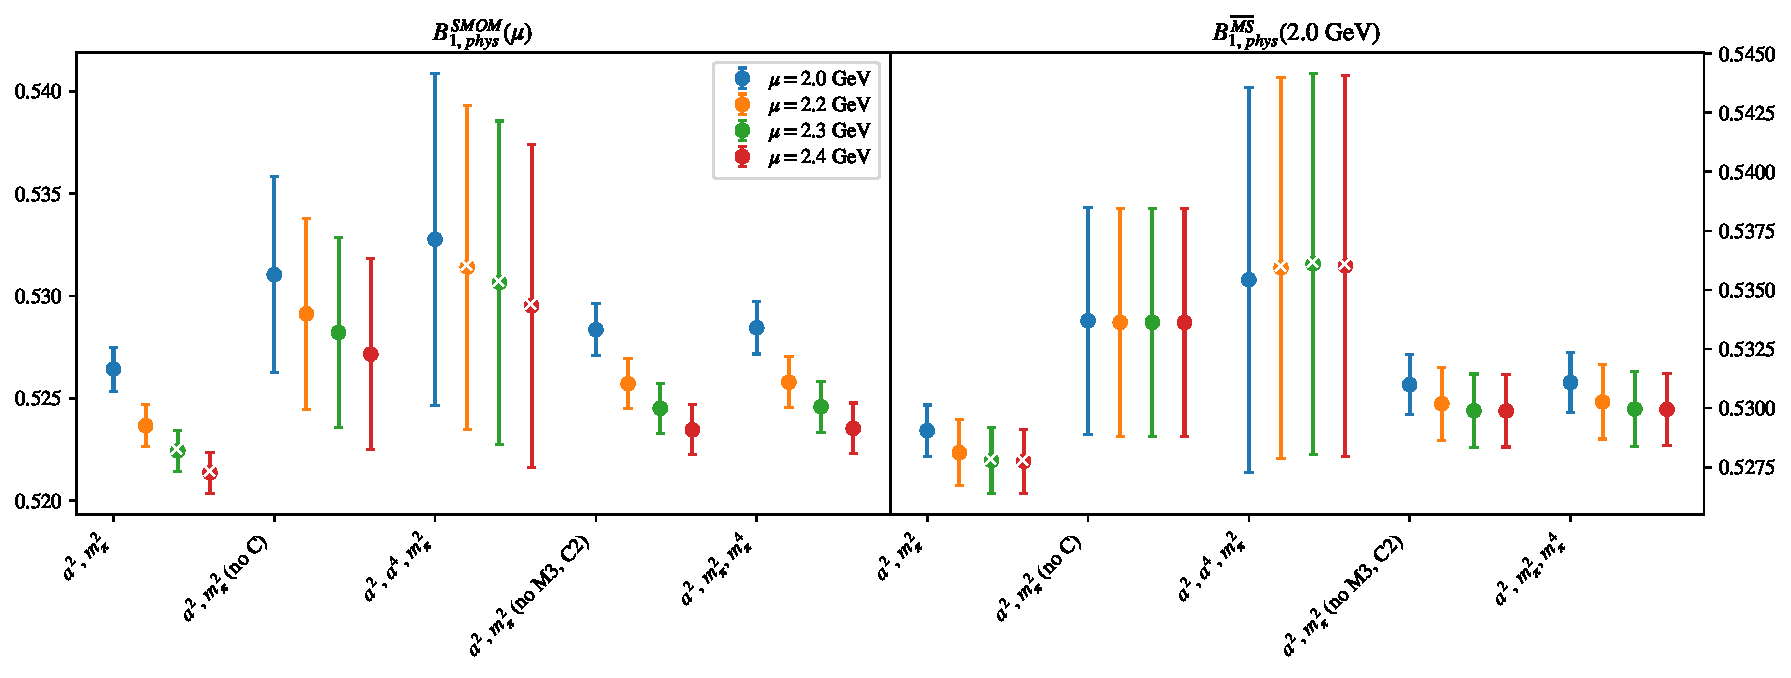
\includegraphics[page=1, width=1.1\textwidth]{VVpAA/NPR/fit_summary.pdf}
\caption{$B_{1}$\\(left) $B_{phys}$ in RI/SMOM scheme from fit variations (fits with $p$-value $<0.05$ marked with ``$\times$"). \\(right) $B_{phys}$ in $\overline{MS}$ computed using $B^{\overline{MS}} = R^{\overline{MS}\leftarrow SMOM}(3.0)\sigma_{npt}^{F1M}(3.0,\mu) B^{SMOM}(\mu)$.}
\end{figure}
\clearpage
\begin{figure}
\centering
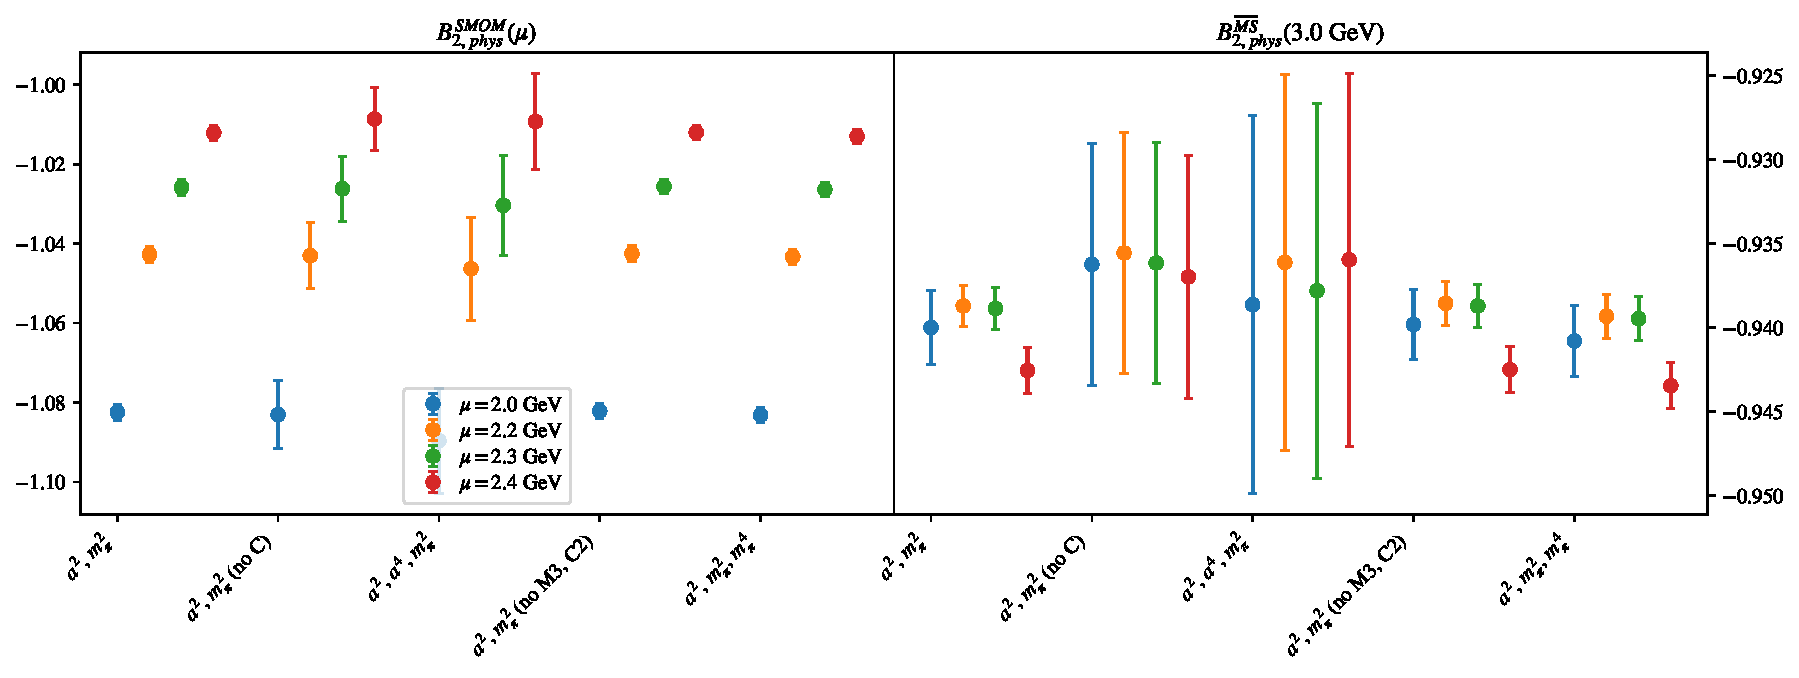
\includegraphics[page=1, width=1.1\textwidth]{VVmAA/NPR/fit_summary.pdf}
\caption{$B_{2}$\\(left) $B_{phys}$ in RI/SMOM scheme from fit variations (fits with $p$-value $<0.05$ marked with ``$\times$"). \\(right) $B_{phys}$ in $\overline{MS}$ computed using $B^{\overline{MS}} = R^{\overline{MS}\leftarrow SMOM}(3.0)\sigma_{npt}^{F1M}(3.0,\mu) B^{SMOM}(\mu)$.}
\end{figure}
\clearpage
\begin{figure}
\centering
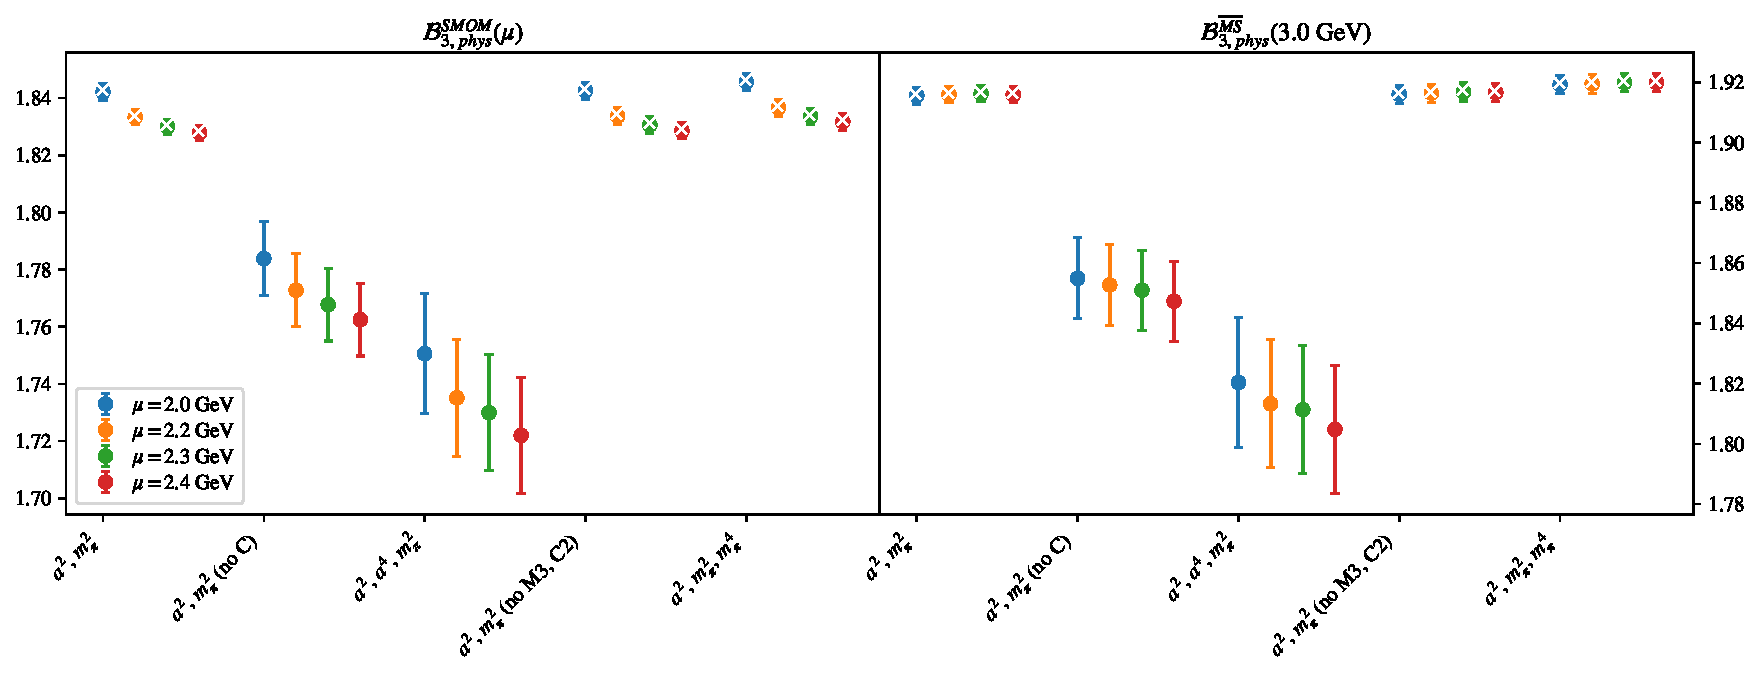
\includegraphics[page=1, width=1.1\textwidth]{SSmPP/NPR/fit_summary.pdf}
\caption{$B_{3}$\\(left) $B_{phys}$ in RI/SMOM scheme from fit variations (fits with $p$-value $<0.05$ marked with ``$\times$"). \\(right) $B_{phys}$ in $\overline{MS}$ computed using $B^{\overline{MS}} = R^{\overline{MS}\leftarrow SMOM}(3.0)\sigma_{npt}^{F1M}(3.0,\mu) B^{SMOM}(\mu)$.}
\end{figure}
\clearpage
\begin{figure}
\centering
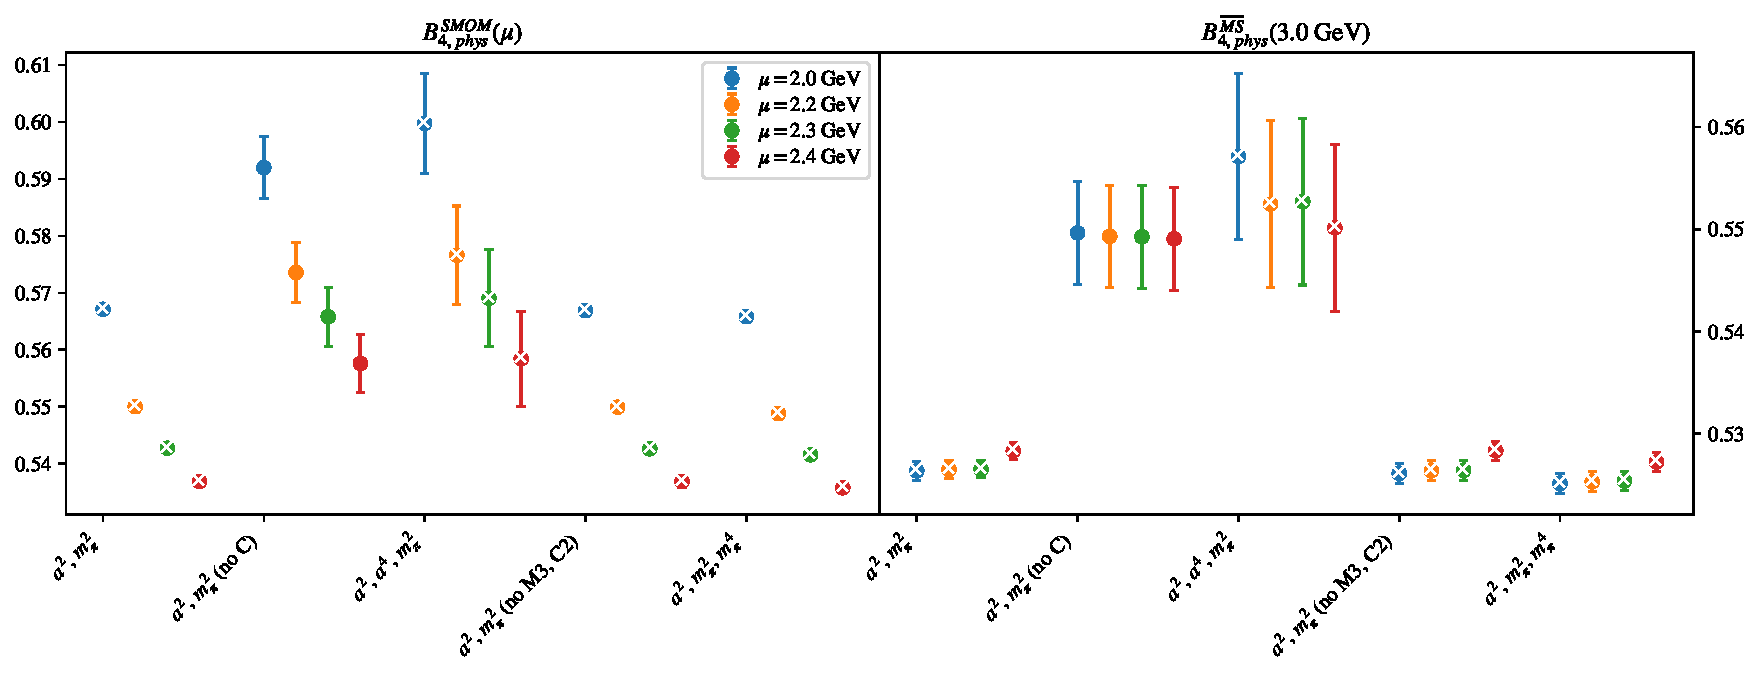
\includegraphics[page=1, width=1.1\textwidth]{SSpPP/NPR/fit_summary.pdf}
\caption{$B_{4}$\\(left) $B_{phys}$ in RI/SMOM scheme from fit variations (fits with $p$-value $<0.05$ marked with ``$\times$"). \\(right) $B_{phys}$ in $\overline{MS}$ computed using $B^{\overline{MS}} = R^{\overline{MS}\leftarrow SMOM}(3.0)\sigma_{npt}^{F1M}(3.0,\mu) B^{SMOM}(\mu)$.}
\end{figure}
\clearpage
\begin{figure}
\centering
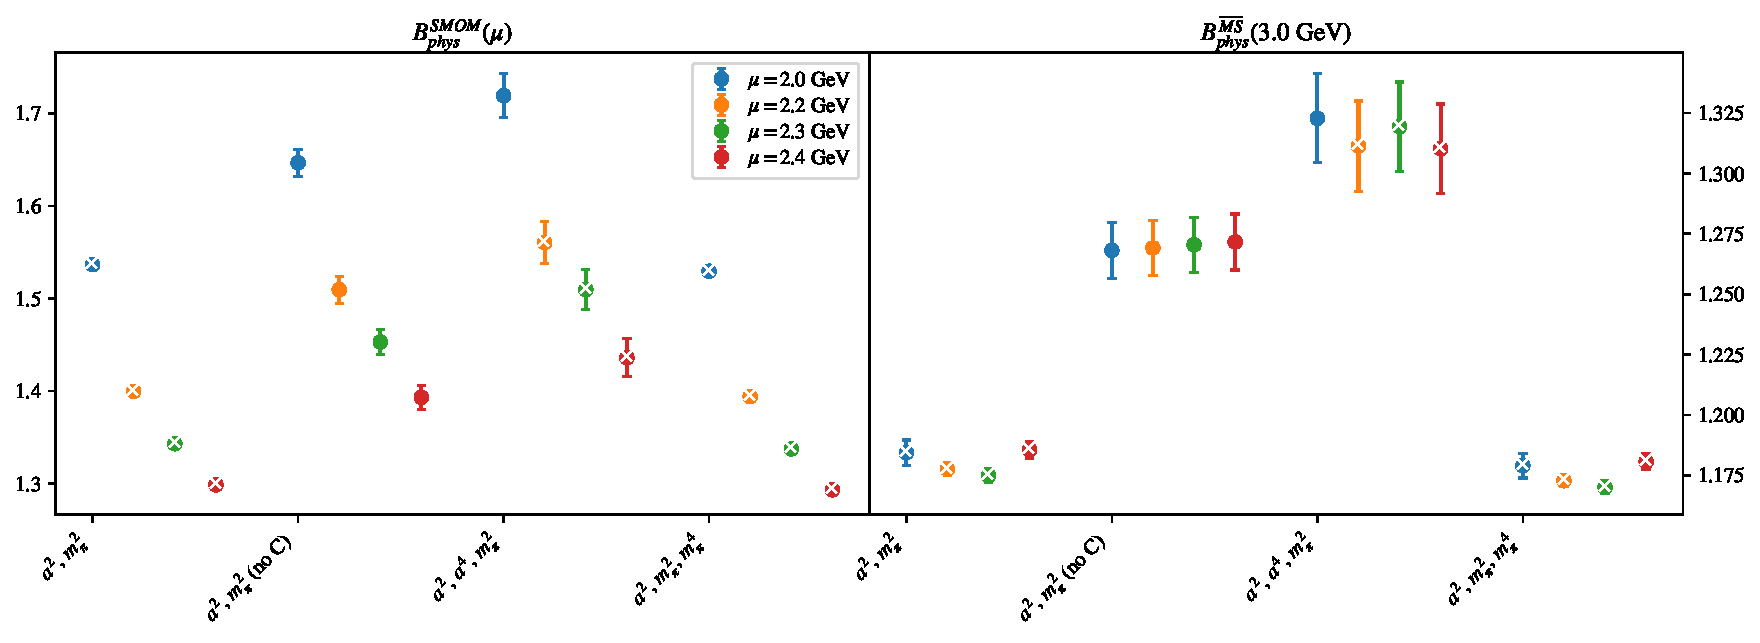
\includegraphics[page=1, width=1.1\textwidth]{TT/NPR/fit_summary.pdf}
\caption{$B_{5}$\\(left) $B_{phys}$ in RI/SMOM scheme from fit variations (fits with $p$-value $<0.05$ marked with ``$\times$"). \\(right) $B_{phys}$ in $\overline{MS}$ computed using $B^{\overline{MS}} = R^{\overline{MS}\leftarrow SMOM}(3.0)\sigma_{npt}^{F1M}(3.0,\mu) B^{SMOM}(\mu)$.}
\end{figure}
\clearpage
\section{$B_1$}
\begin{table}[h!]
\begin{center}
\begin{tabular}{|c|c|c|c|c|c|}
\hline
$\mu$ (GeV) & $a^2$, $m_\pi^2$& $a^2$, $m_\pi^2$ (no C)& $a^2$, $a^4$, $m_\pi^2$& $a^2$, $m_\pi^2$, $m_\pi^4$& $a^2$, $m_\pi^2$, $\log(m_\pi^2/\Lambda^2)$\\
\hline
2.4& \hyperlink{VVpAA/NPR/a2m2_24.pdf.1}{\textbf{0.5213(10)}: 2.342 (0.039)} & \hyperlink{VVpAA/NPR/a2m2noC_24.pdf.1}{\textbf{0.5271(46)}: 1.22 (0.295)} & \hyperlink{VVpAA/NPR/a2a4m2_24.pdf.1}{\textbf{0.5294(79)}: 2.664 (0.031)} & \hyperlink{VVpAA/NPR/a2m2m4_24.pdf.1}{\textbf{0.5233(12)}: 0.993 (0.41)} & \hyperlink{VVpAA/NPR/a2m2logm2_24.pdf.1}{\textbf{0.51075(99)}: 9.014 (0.0)}\\
2.0& \hyperlink{VVpAA/NPR/a2m2_20.pdf.1}{\textbf{0.5264(11)}: 1.838 (0.102)} & \hyperlink{VVpAA/NPR/a2m2noC_20.pdf.1}{\textbf{0.5310(48)}: 0.864 (0.421)} & \hyperlink{VVpAA/NPR/a2a4m2_20.pdf.1}{\textbf{0.5326(82)}: 2.159 (0.071)} & \hyperlink{VVpAA/NPR/a2m2m4_20.pdf.1}{\textbf{0.5282(12)}: 0.639 (0.635)} & \hyperlink{VVpAA/NPR/a2m2logm2_20.pdf.1}{\textbf{0.5157(10)}: 8.193 (0.0)}\\
1.8& \hyperlink{VVpAA/NPR/a2m2_18.pdf.1}{\textbf{0.5293(14)}: 1.315 (0.254)} & \hyperlink{VVpAA/NPR/a2m2noC_18.pdf.1}{\textbf{0.5328(53)}: 0.478 (0.62)} & \hyperlink{VVpAA/NPR/a2a4m2_18.pdf.1}{\textbf{0.5335(91)}: 1.6 (0.171)} & \hyperlink{VVpAA/NPR/a2m2m4_18.pdf.1}{\textbf{0.5310(14)}: 0.307 (0.873)} & \hyperlink{VVpAA/NPR/a2m2logm2_18.pdf.1}{\textbf{0.5188(13)}: 6.778 (0.0)}\\
1.5& \hyperlink{VVpAA/NPR/a2m2_15.pdf.1}{\textbf{0.5338(19)}: 0.734 (0.598)} & \hyperlink{VVpAA/NPR/a2m2noC_15.pdf.1}{\textbf{0.5356(64)}: 0.159 (0.853)} & \hyperlink{VVpAA/NPR/a2a4m2_15.pdf.1}{\textbf{0.536(11)}: 0.909 (0.457)} & \hyperlink{VVpAA/NPR/a2m2m4_15.pdf.1}{\textbf{0.5352(18)}: 0.099 (0.983)} & \hyperlink{VVpAA/NPR/a2m2logm2_15.pdf.1}{\textbf{0.5237(19)}: 4.464 (0.0)}\\
\hline
\end{tabular}
\caption{Physical point value from chiral and continuum extrapolation at renormalisation scale $\mu$. Entries are \textbf{value(error)}: $\chi^2/\text{DOF}$ ($p$-value).}
\end{center}
\end{table}
\begin{table}[h!]
\begin{center}
\begin{tabular}{|c c|c|c|c|c|c|}
\hline
$\mu$ (GeV) &  & $a^2$, $m_\pi^2$& $a^2$, $m_\pi^2$ (no C)& $a^2$, $a^4$, $m_\pi^2$& $a^2$, $m_\pi^2$, $m_\pi^4$& $a^2$, $m_\pi^2$, $\log(m_\pi^2/\Lambda^2)$\\
\hline
\multirow{2}{0.5in}{2.4} & $\alpha$ & 0.1001(70)& 0.040(52)& -0.043& 0.0864(83)& 0.1218(71)\\
 & $\beta$ & 0.00264(14)& 0.00221(27)& 0.00268(15)& 0.00016(89)& -0.0019(15)\\
\hline
\multirow{2}{0.5in}{2.0} & $\alpha$ & 0.0939(73)& 0.047(53)& -0.015& 0.0813(84)& 0.1150(74)\\
 & $\beta$ & 0.00262(14)& 0.00223(28)& 0.00265(15)& 0.00030(90)& -0.0020(15)\\
\hline
\multirow{2}{0.5in}{1.8} & $\alpha$ & 0.0894(84)& 0.055(57)& 0.016& 0.0781(89)& 0.1088(85)\\
 & $\beta$ & 0.00262(15)& 0.00225(29)& 0.00264(15)& 0.00039(94)& -0.0020(15)\\
\hline
\multirow{2}{0.5in}{1.5} & $\alpha$ & 0.081(10)& 0.066(65)& 0.036& 0.0722(99)& 0.098(10)\\
 & $\beta$ & 0.00261(15)& 0.00230(34)& 0.00261(16)& 0.001& -0.0020(15)\\
\hline
\end{tabular}
\caption{Fit values of coefficients in $B = B_0(1 + \mathbf{\alpha} a^2 + \mathbf{\beta} \frac{m_\pi^2}{f_\pi^2} + \ldots)$.}
\end{center}
\end{table}
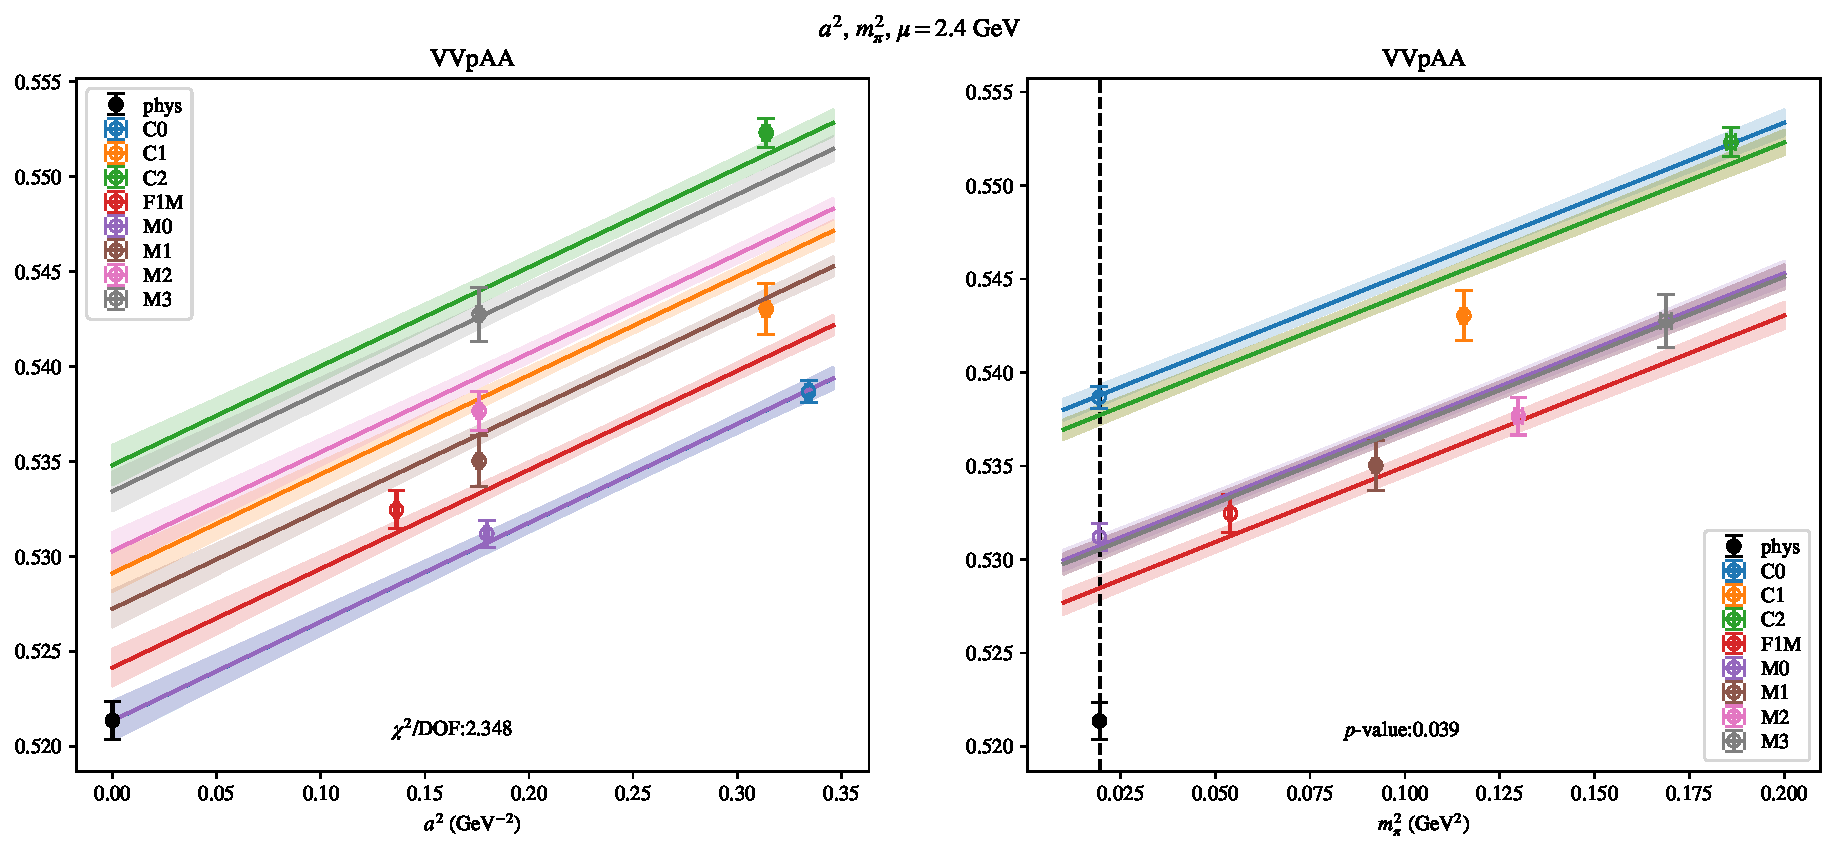
\includepdf[link, pages=-]{VVpAA/NPR/a2m2_24.pdf}
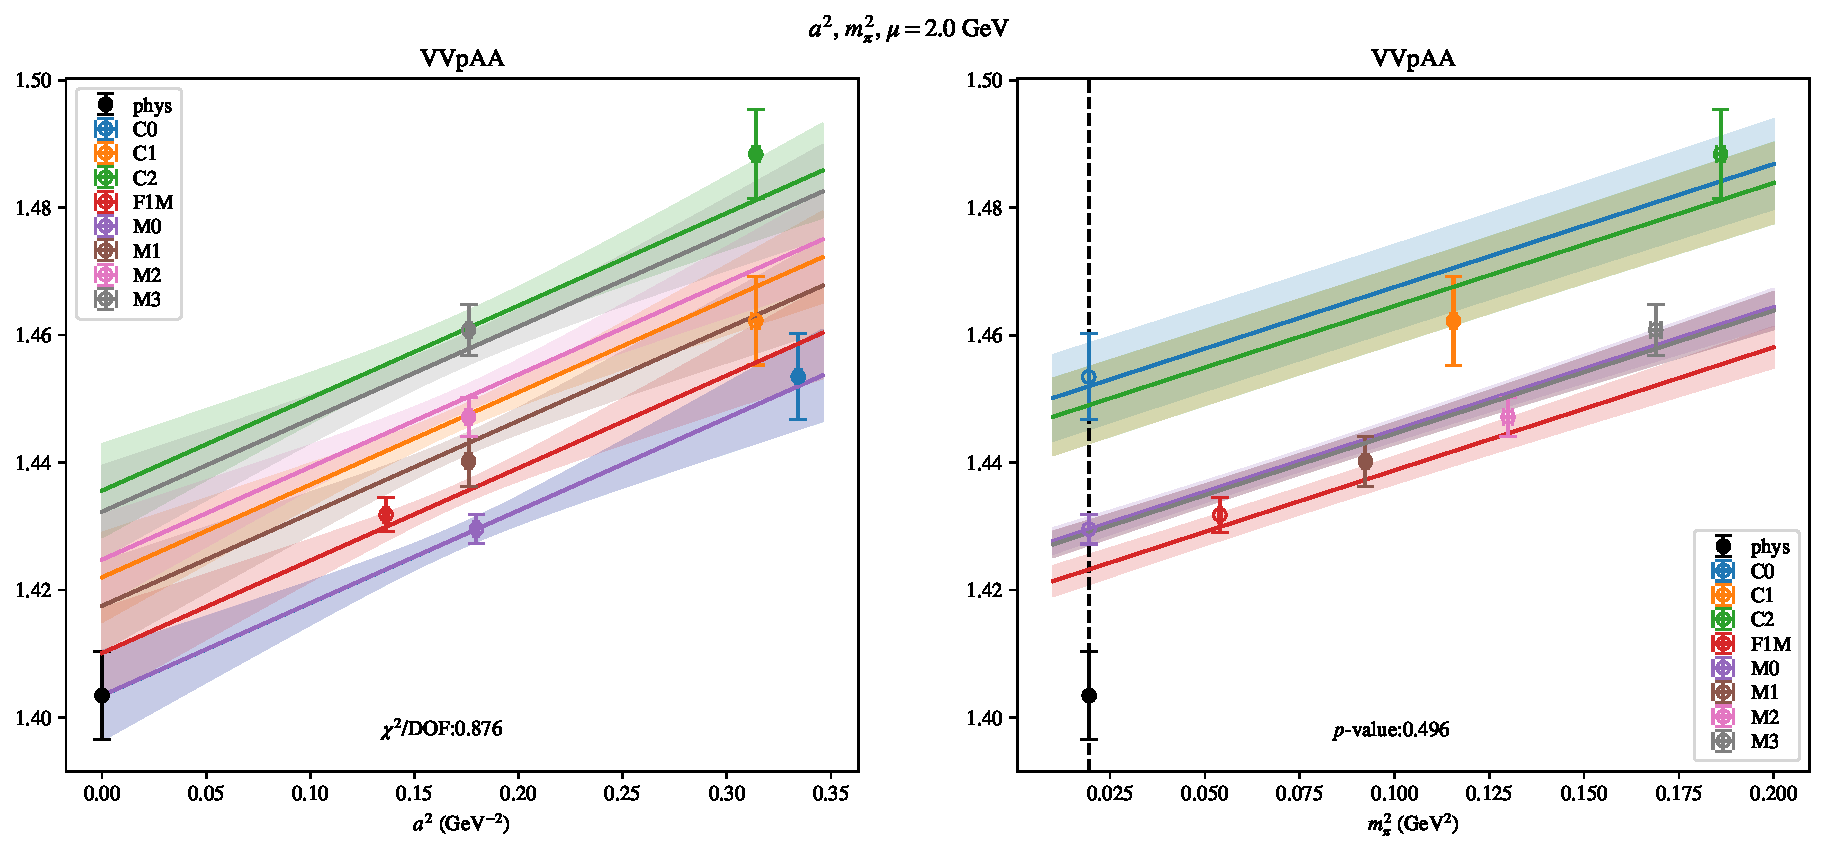
\includepdf[link, pages=-]{VVpAA/NPR/a2m2_20.pdf}
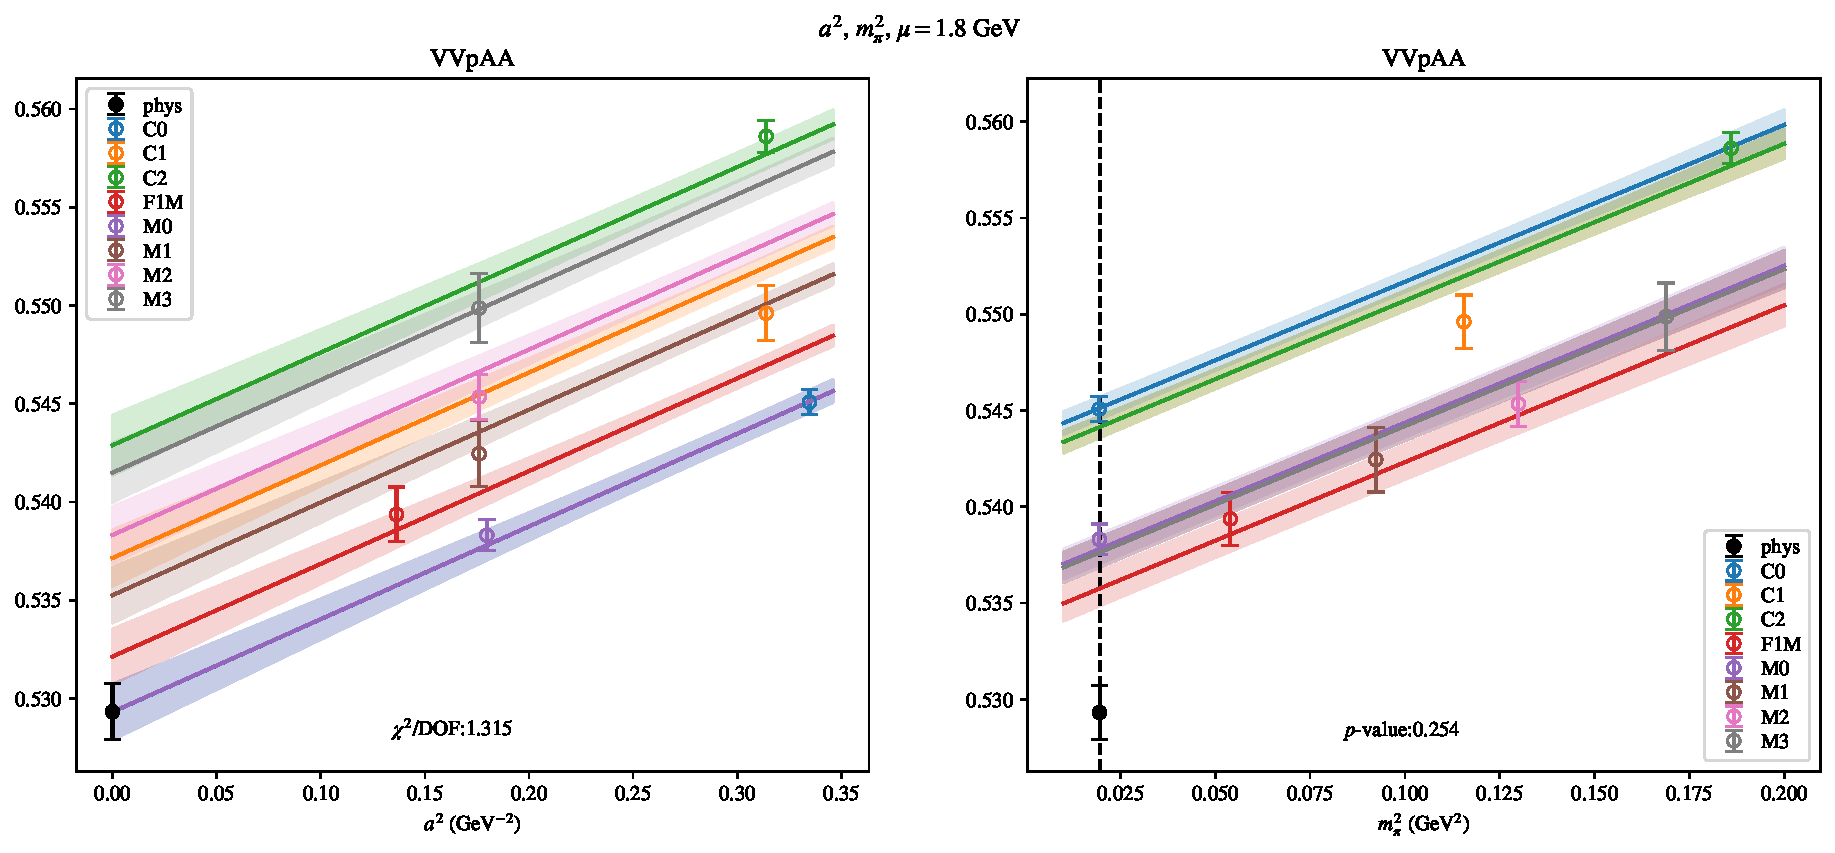
\includepdf[link, pages=-]{VVpAA/NPR/a2m2_18.pdf}
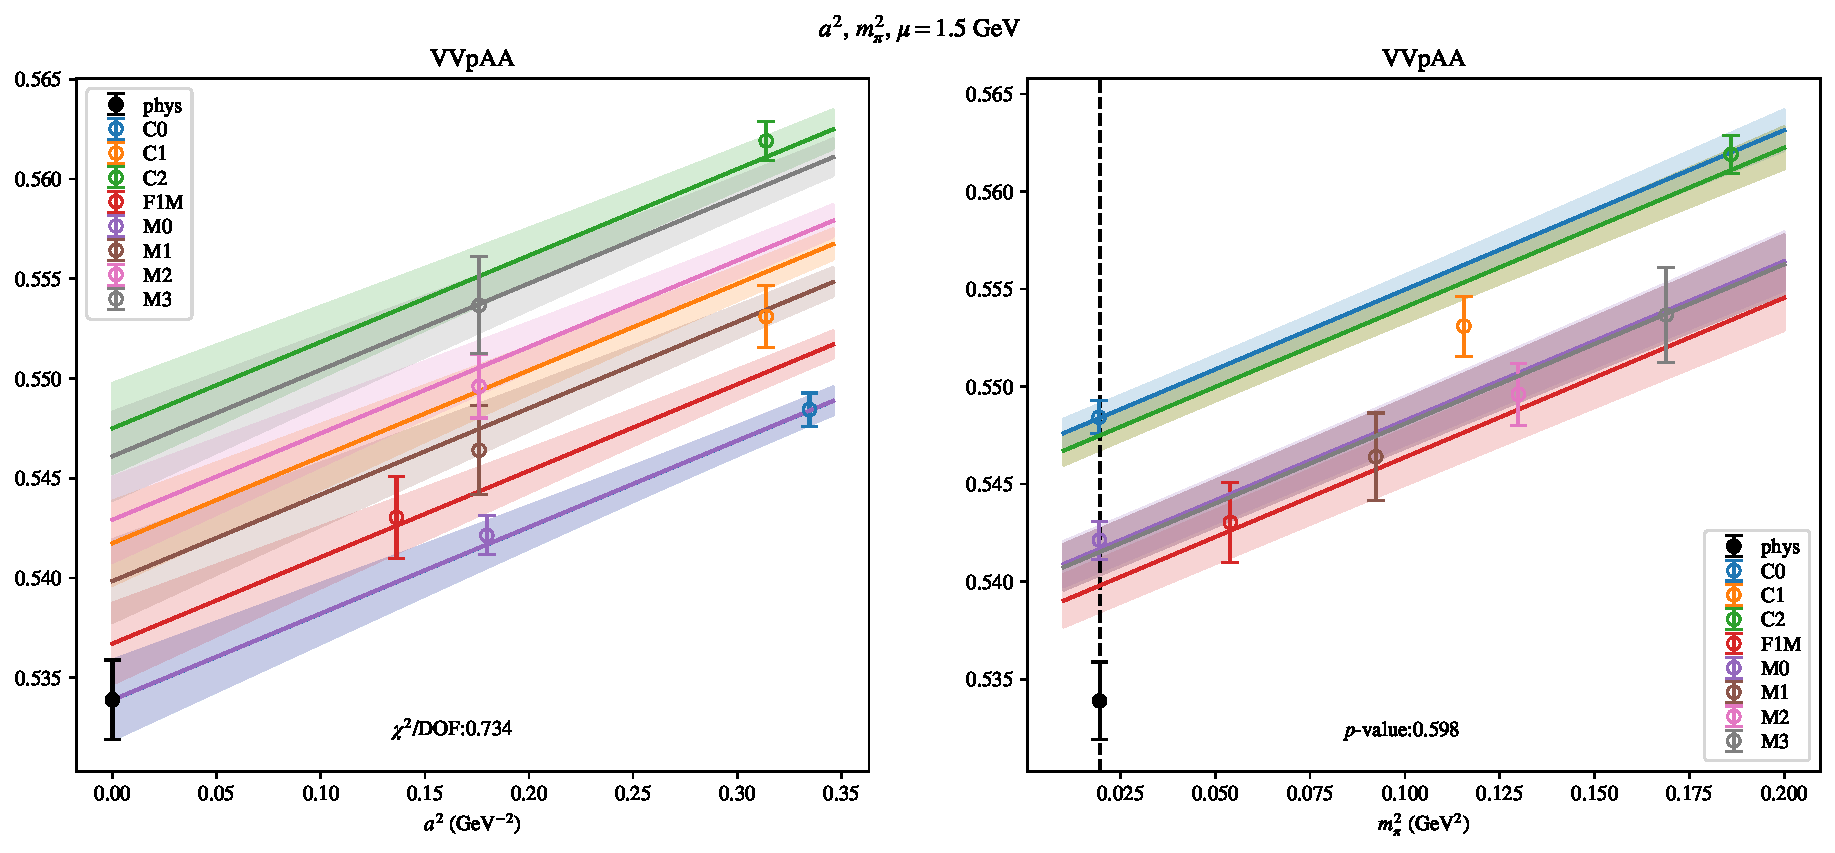
\includepdf[link, pages=-]{VVpAA/NPR/a2m2_15.pdf}
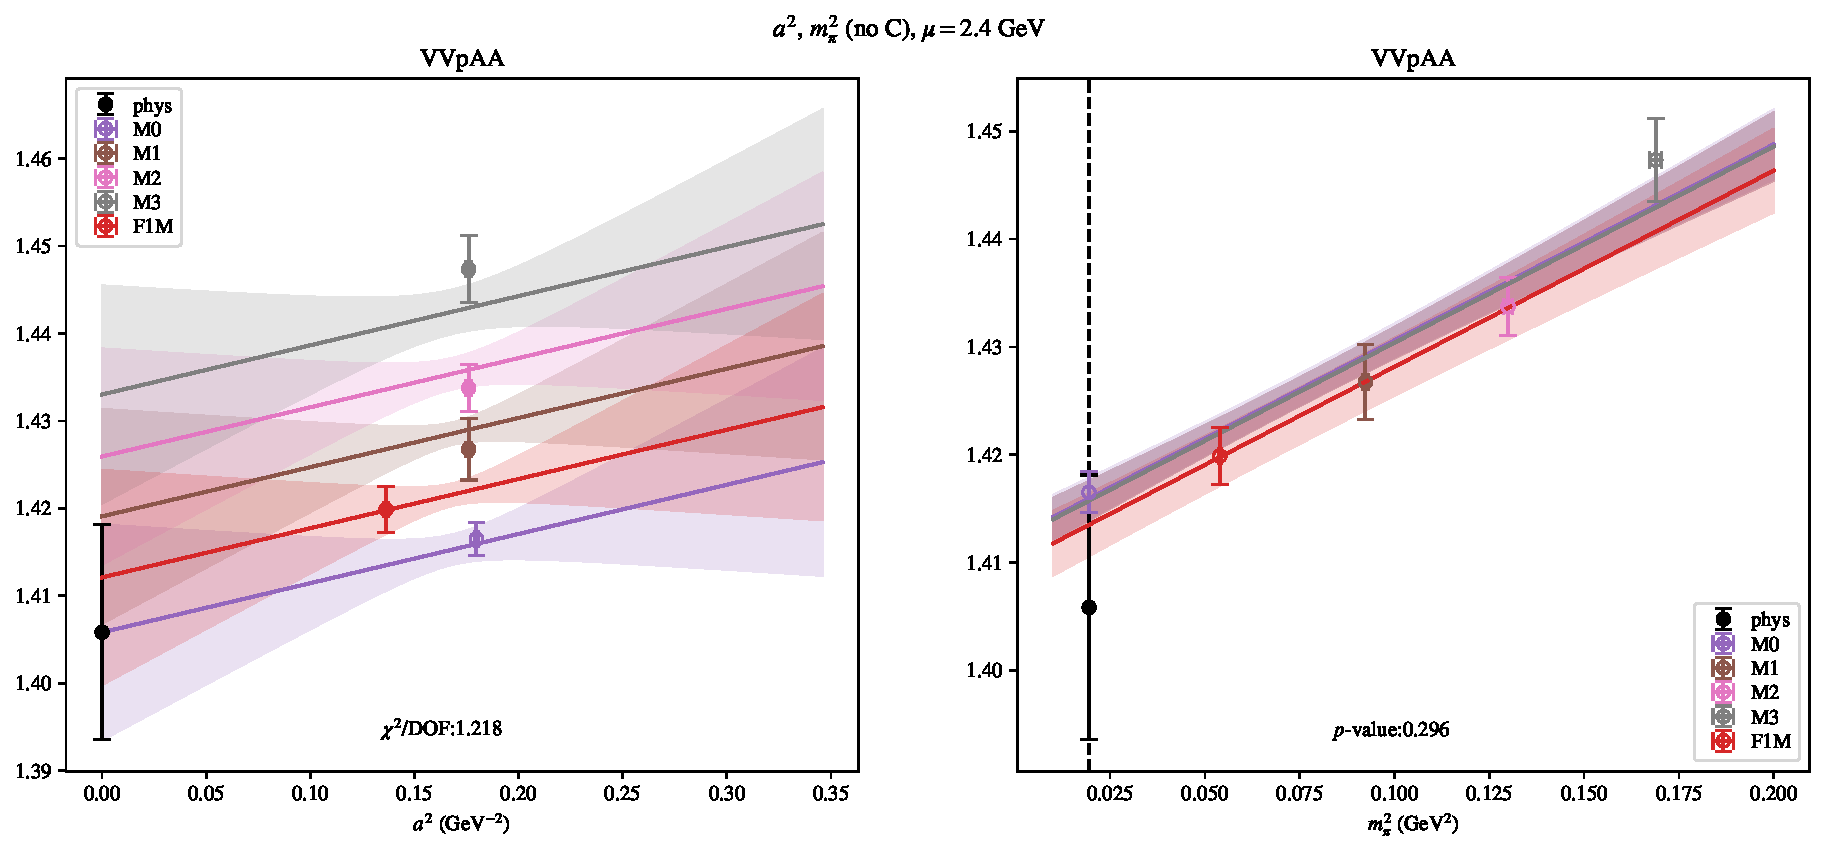
\includepdf[link, pages=-]{VVpAA/NPR/a2m2noC_24.pdf}
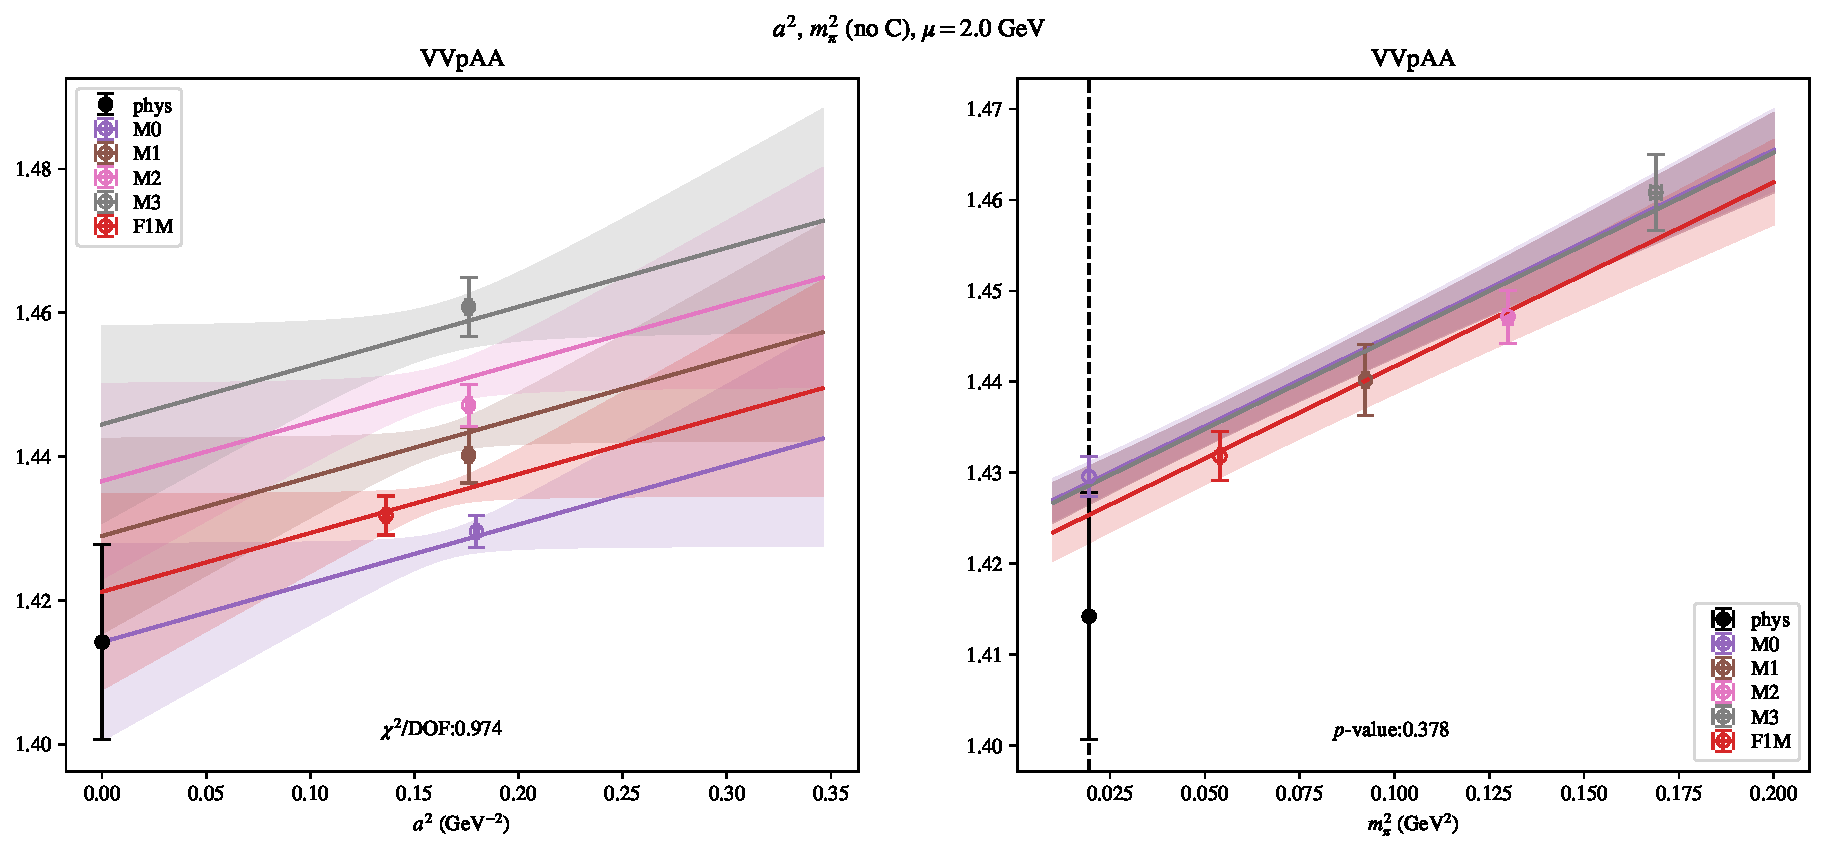
\includepdf[link, pages=-]{VVpAA/NPR/a2m2noC_20.pdf}
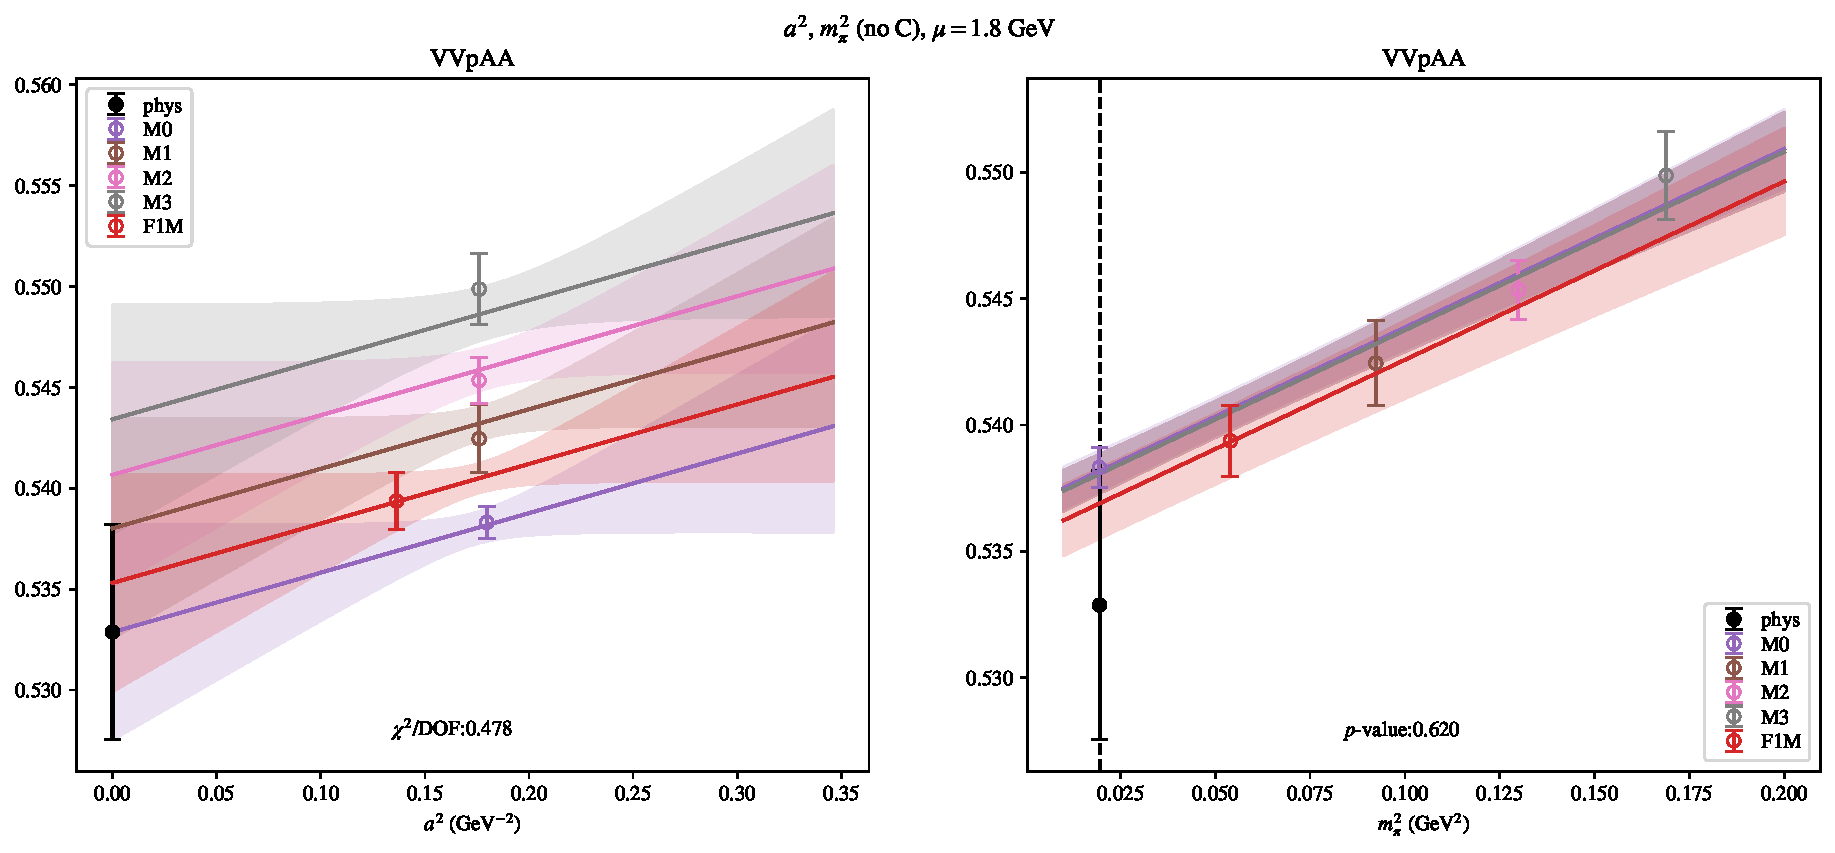
\includepdf[link, pages=-]{VVpAA/NPR/a2m2noC_18.pdf}
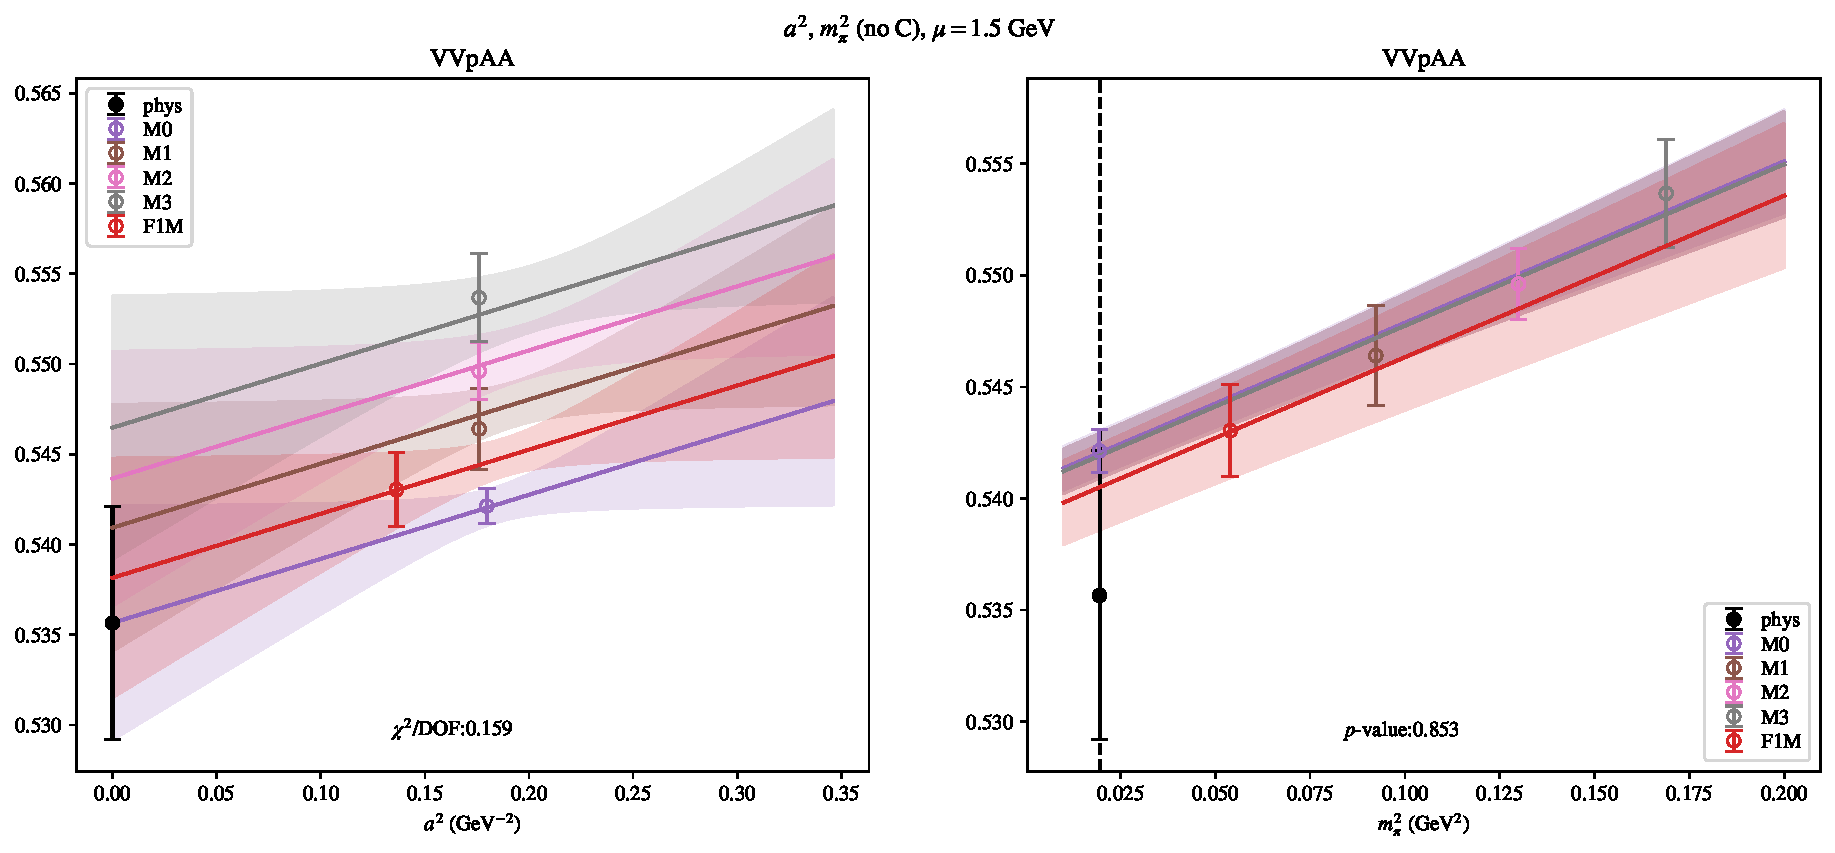
\includepdf[link, pages=-]{VVpAA/NPR/a2m2noC_15.pdf}
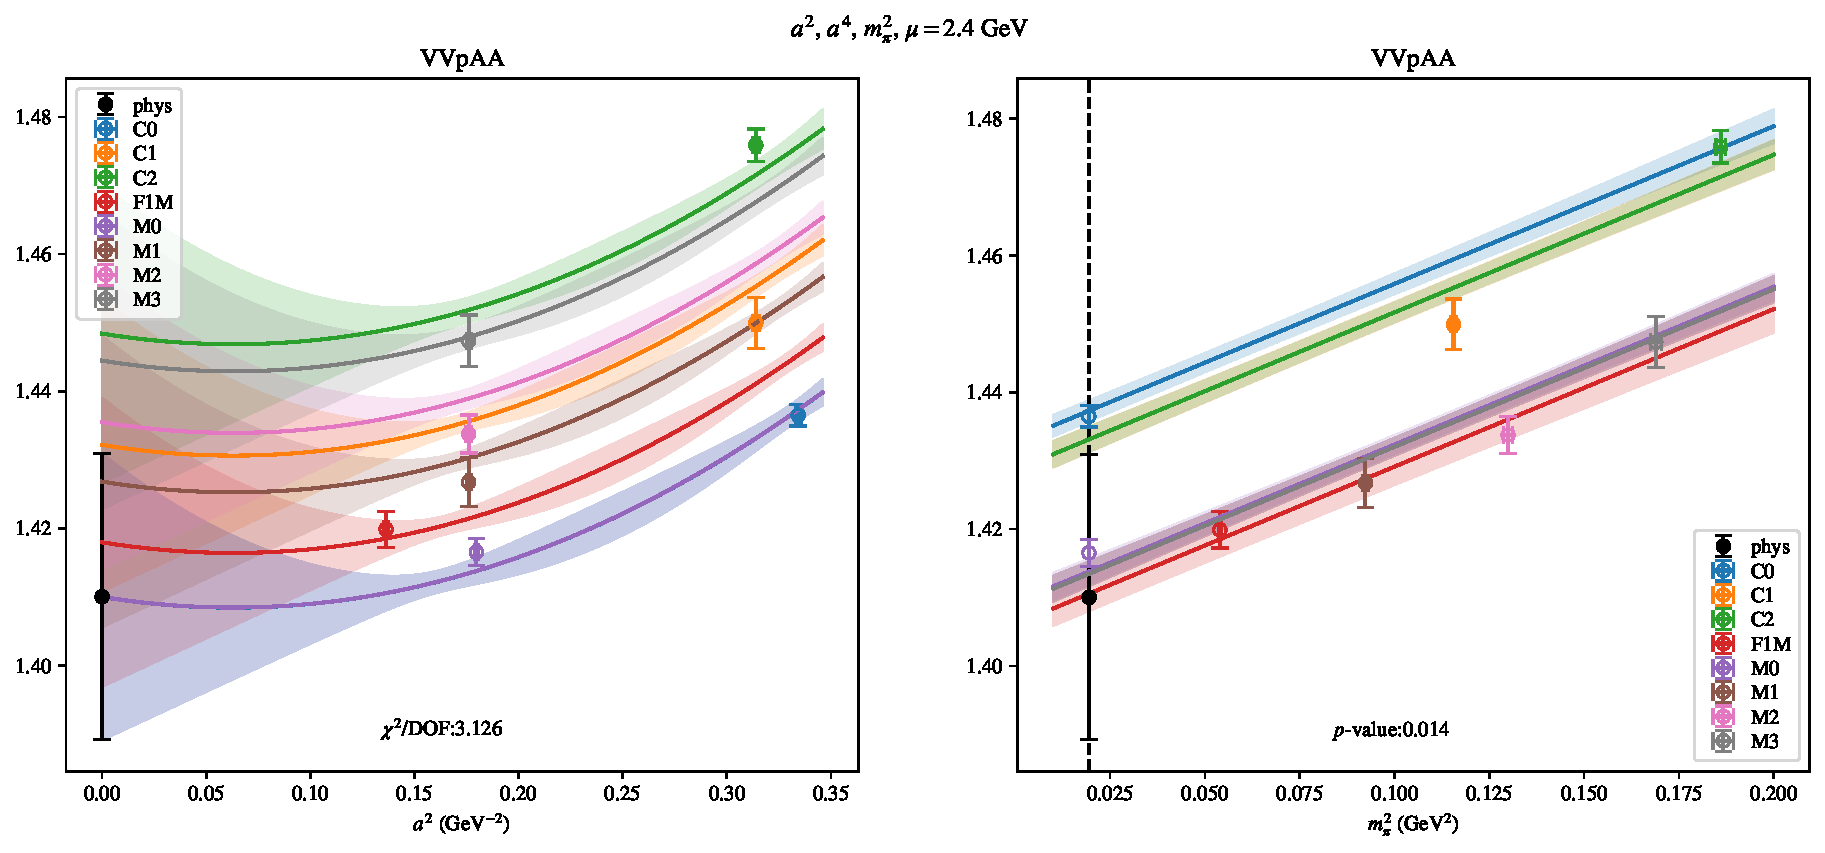
\includepdf[link, pages=-]{VVpAA/NPR/a2a4m2_24.pdf}
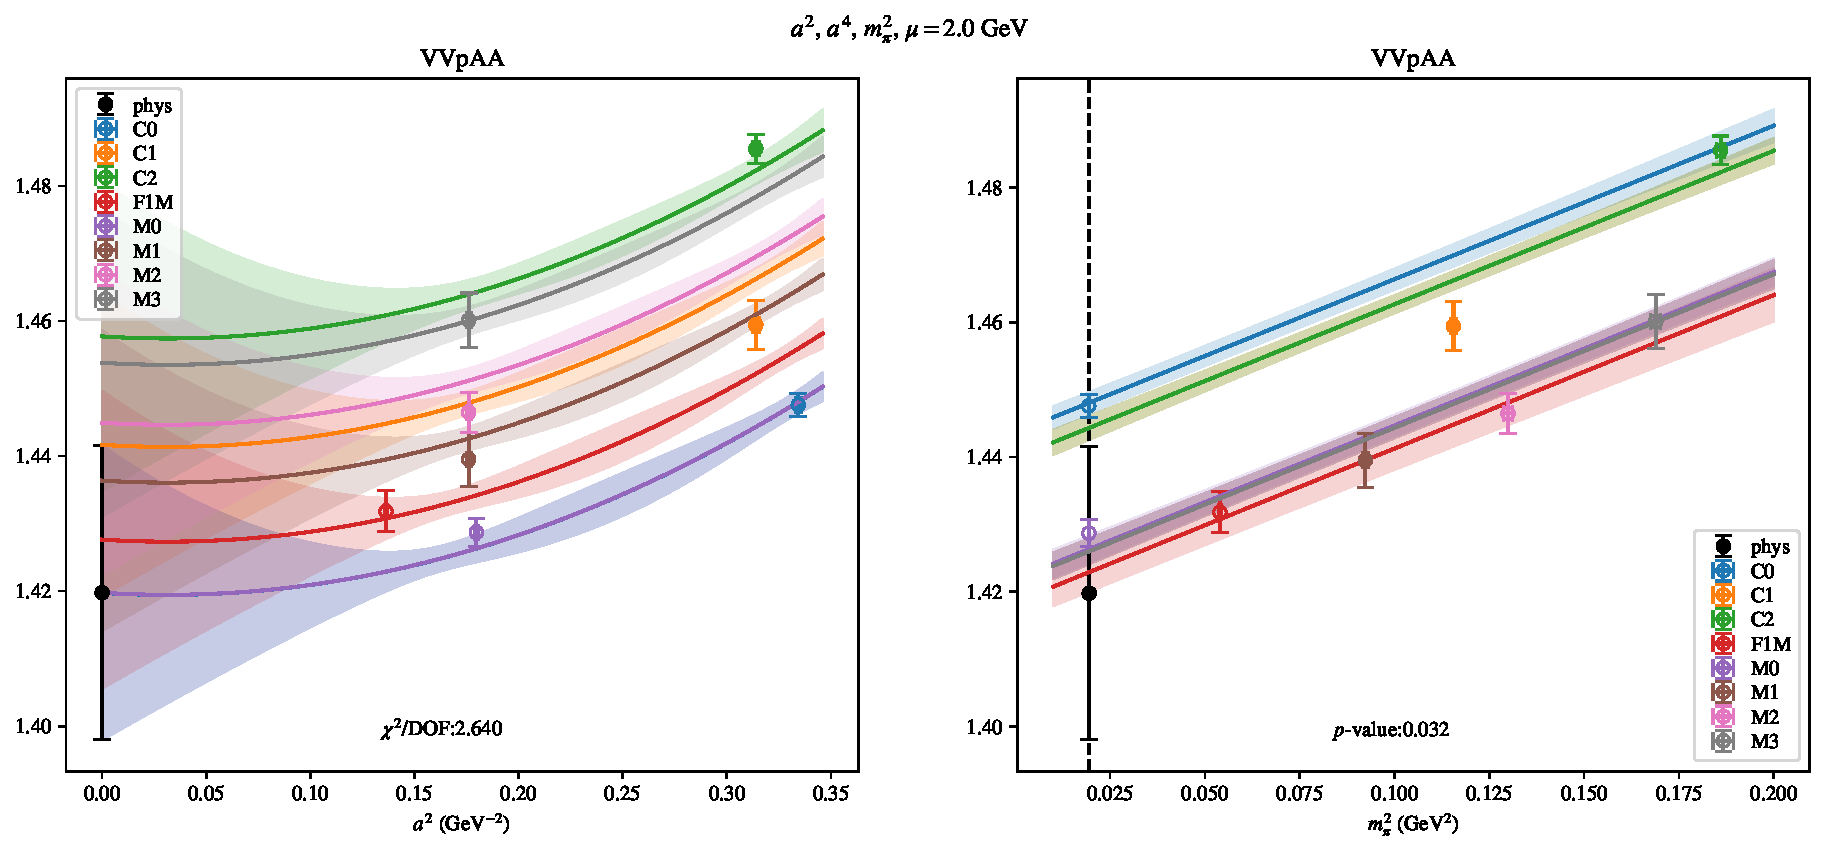
\includepdf[link, pages=-]{VVpAA/NPR/a2a4m2_20.pdf}
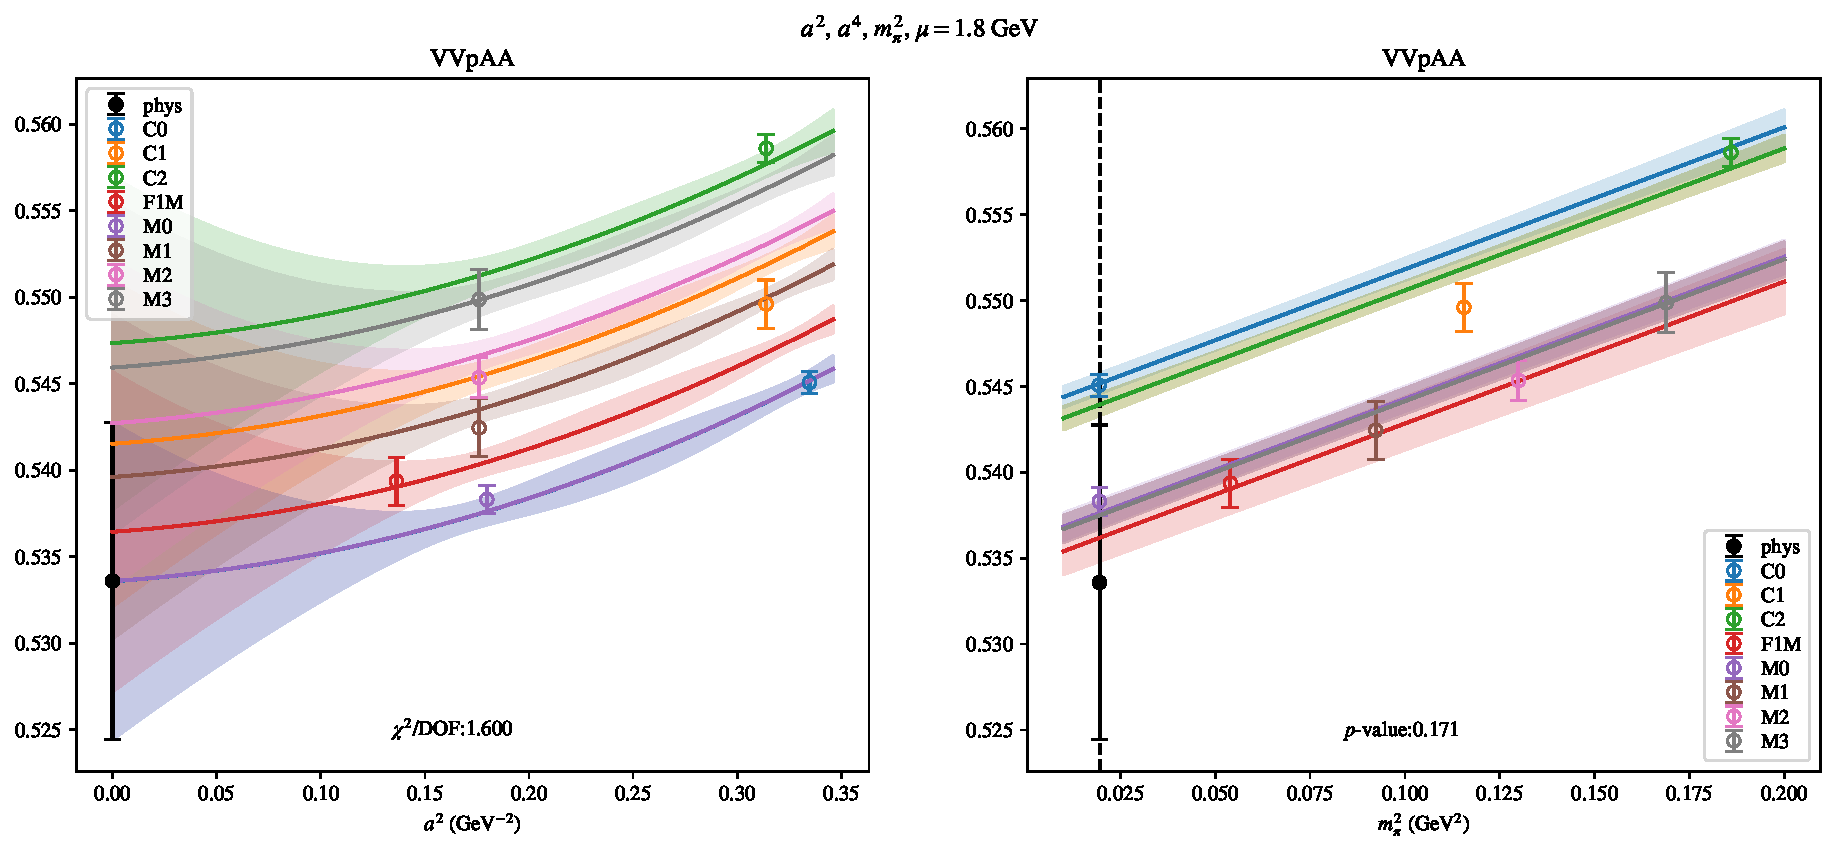
\includepdf[link, pages=-]{VVpAA/NPR/a2a4m2_18.pdf}
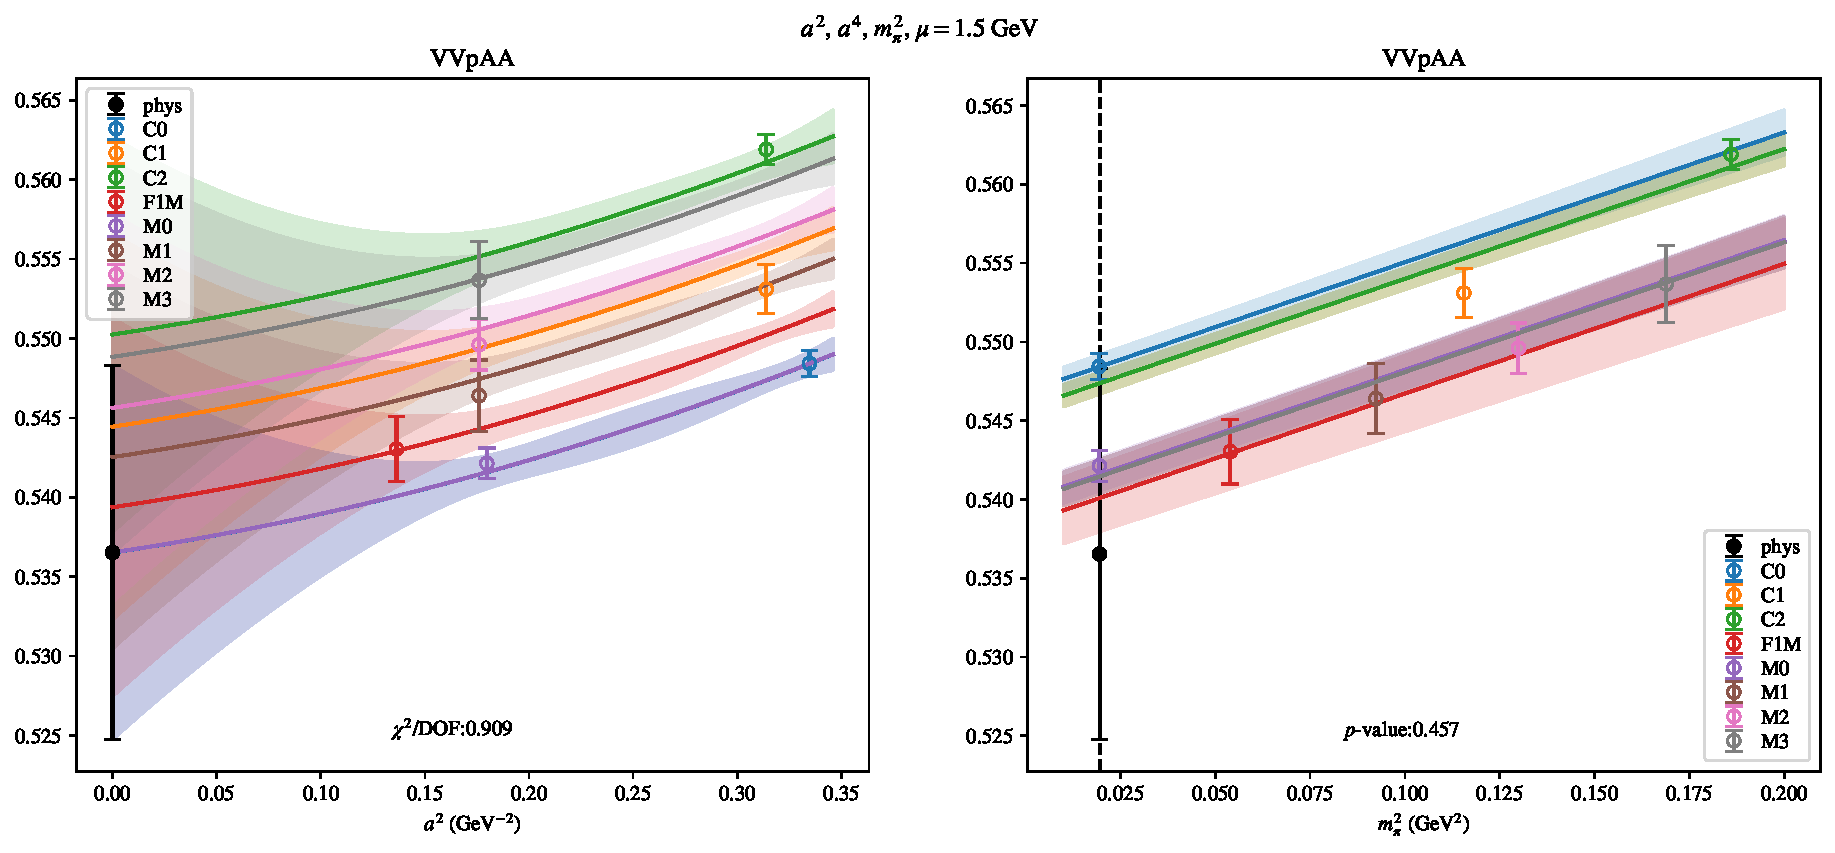
\includepdf[link, pages=-]{VVpAA/NPR/a2a4m2_15.pdf}
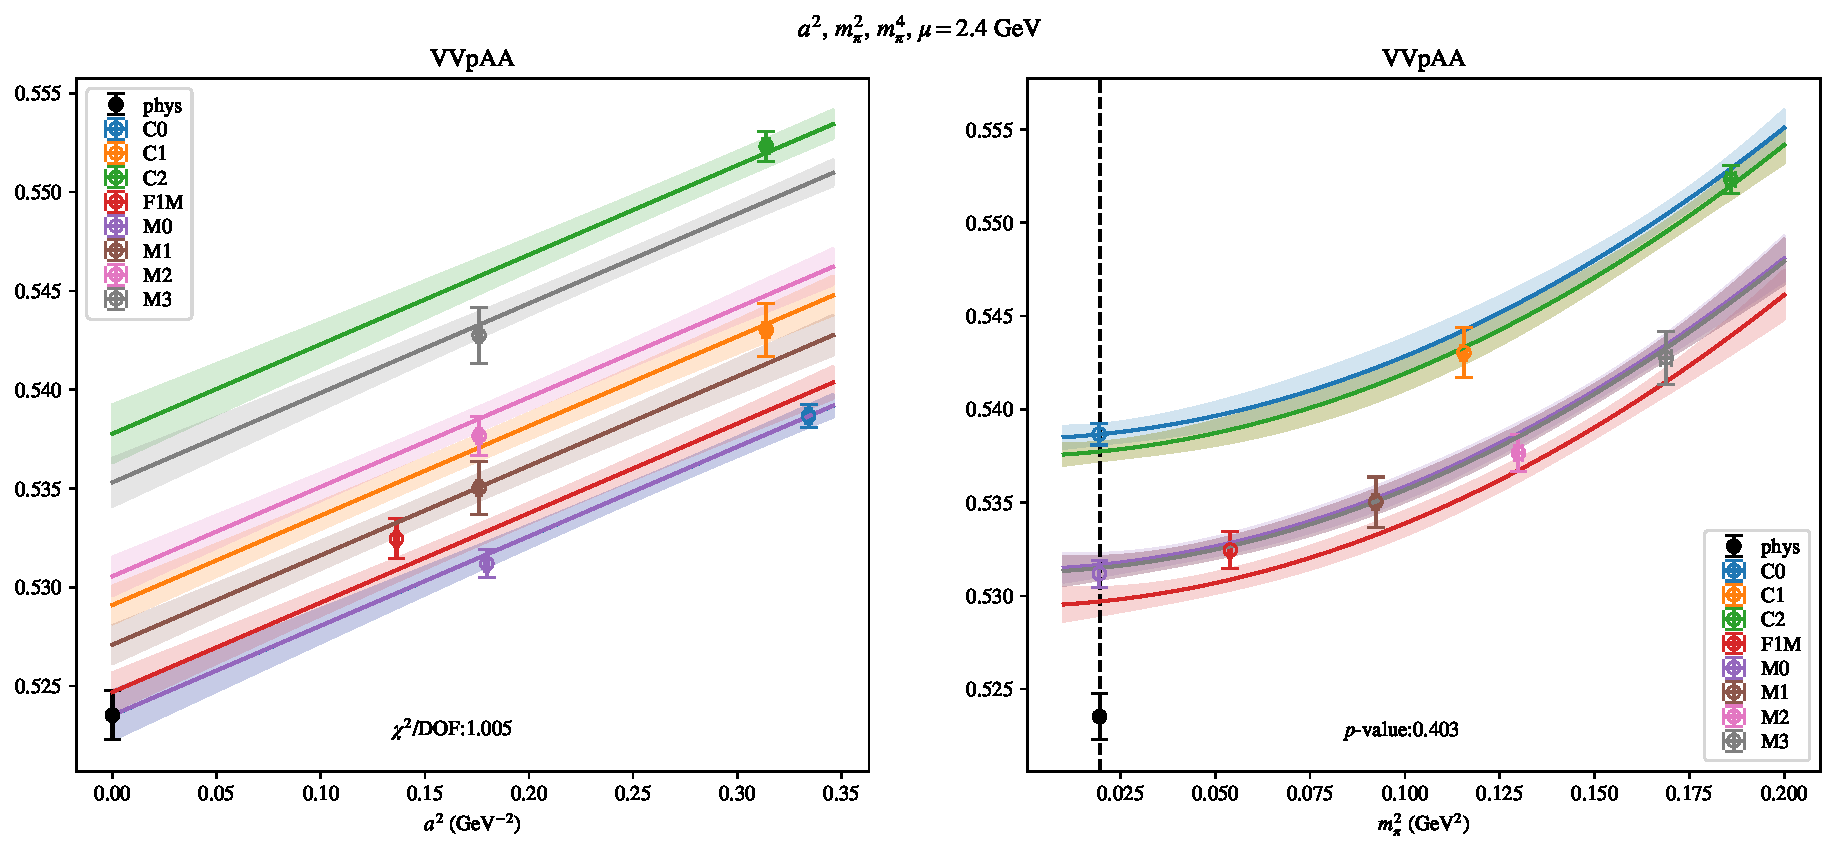
\includepdf[link, pages=-]{VVpAA/NPR/a2m2m4_24.pdf}
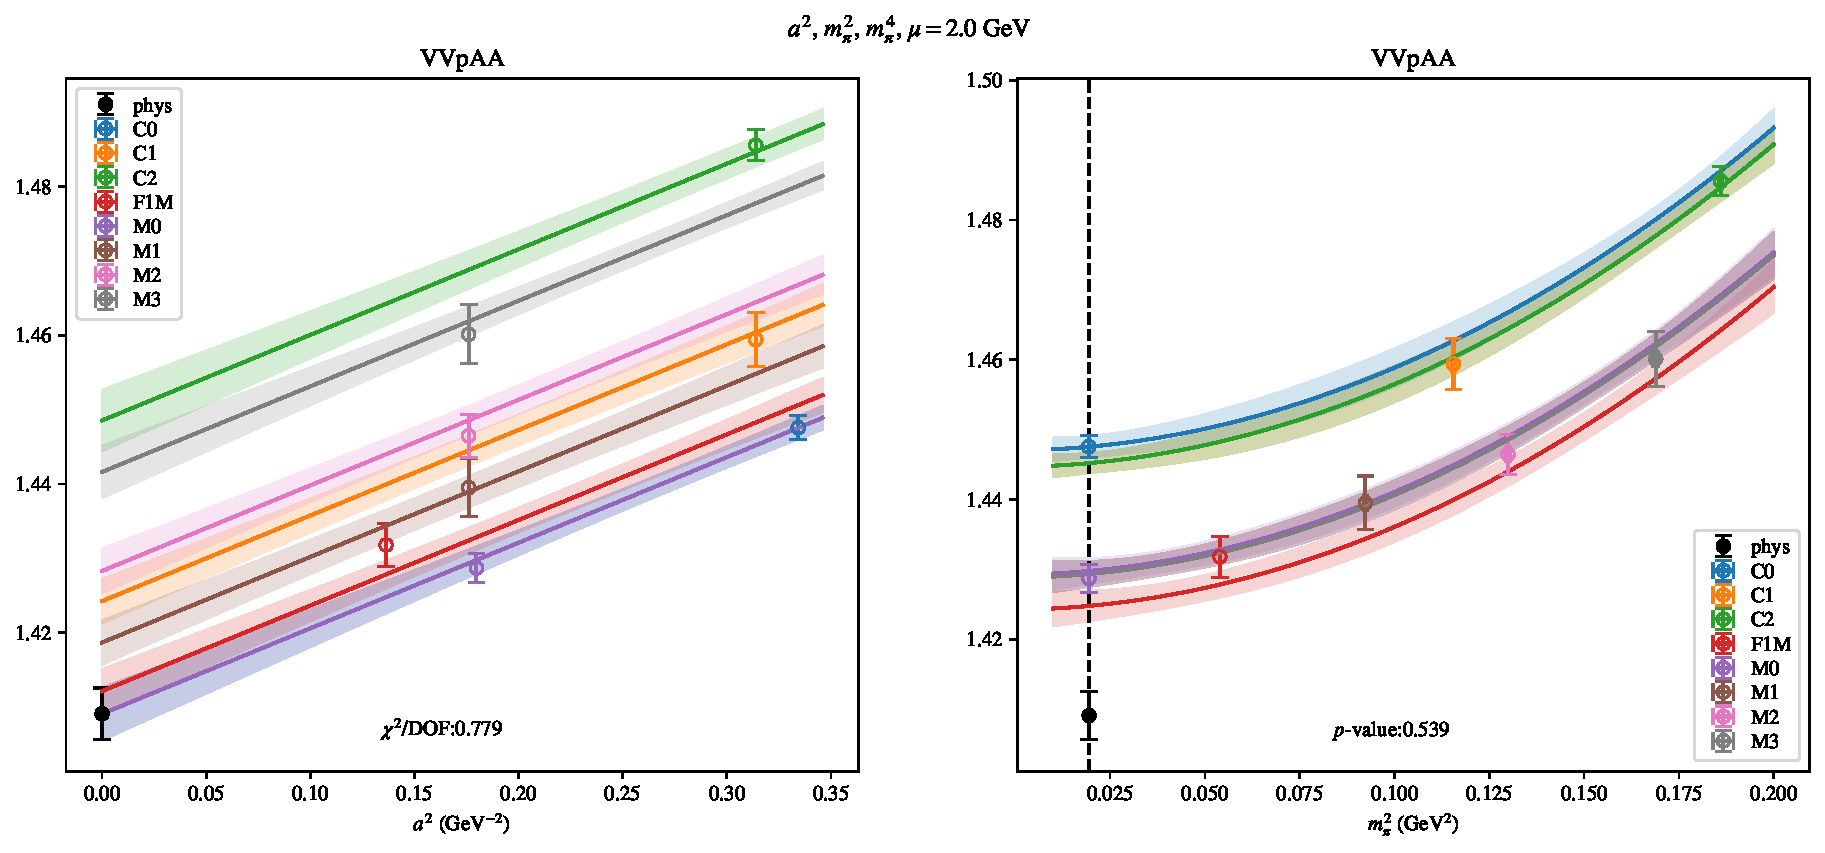
\includepdf[link, pages=-]{VVpAA/NPR/a2m2m4_20.pdf}
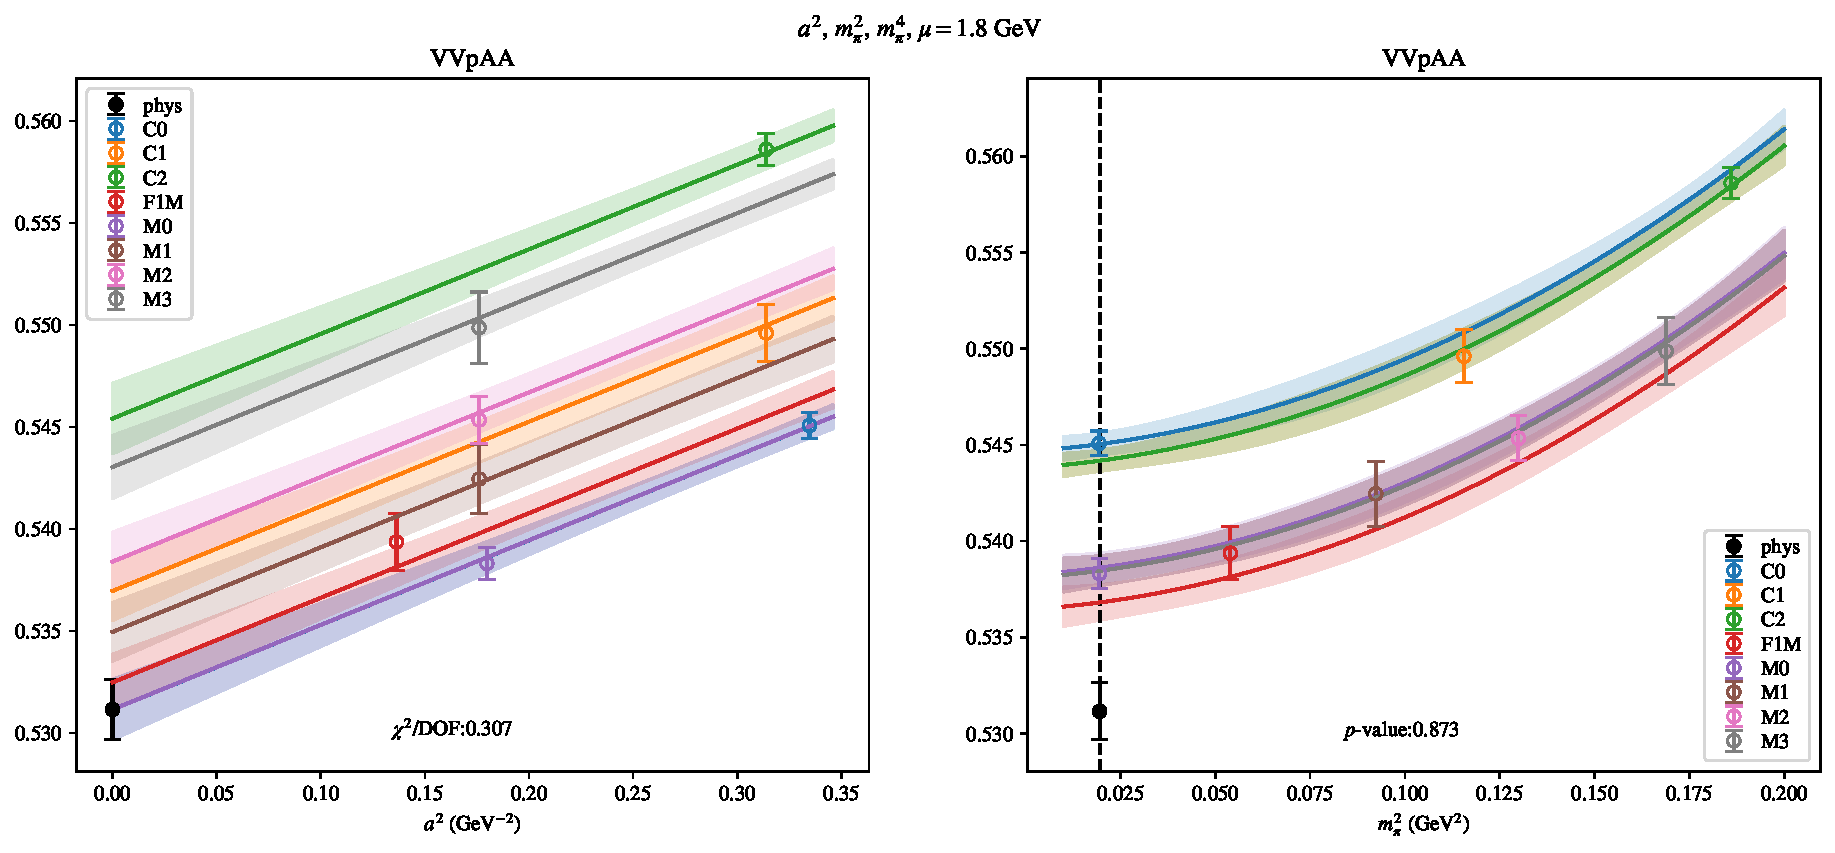
\includepdf[link, pages=-]{VVpAA/NPR/a2m2m4_18.pdf}
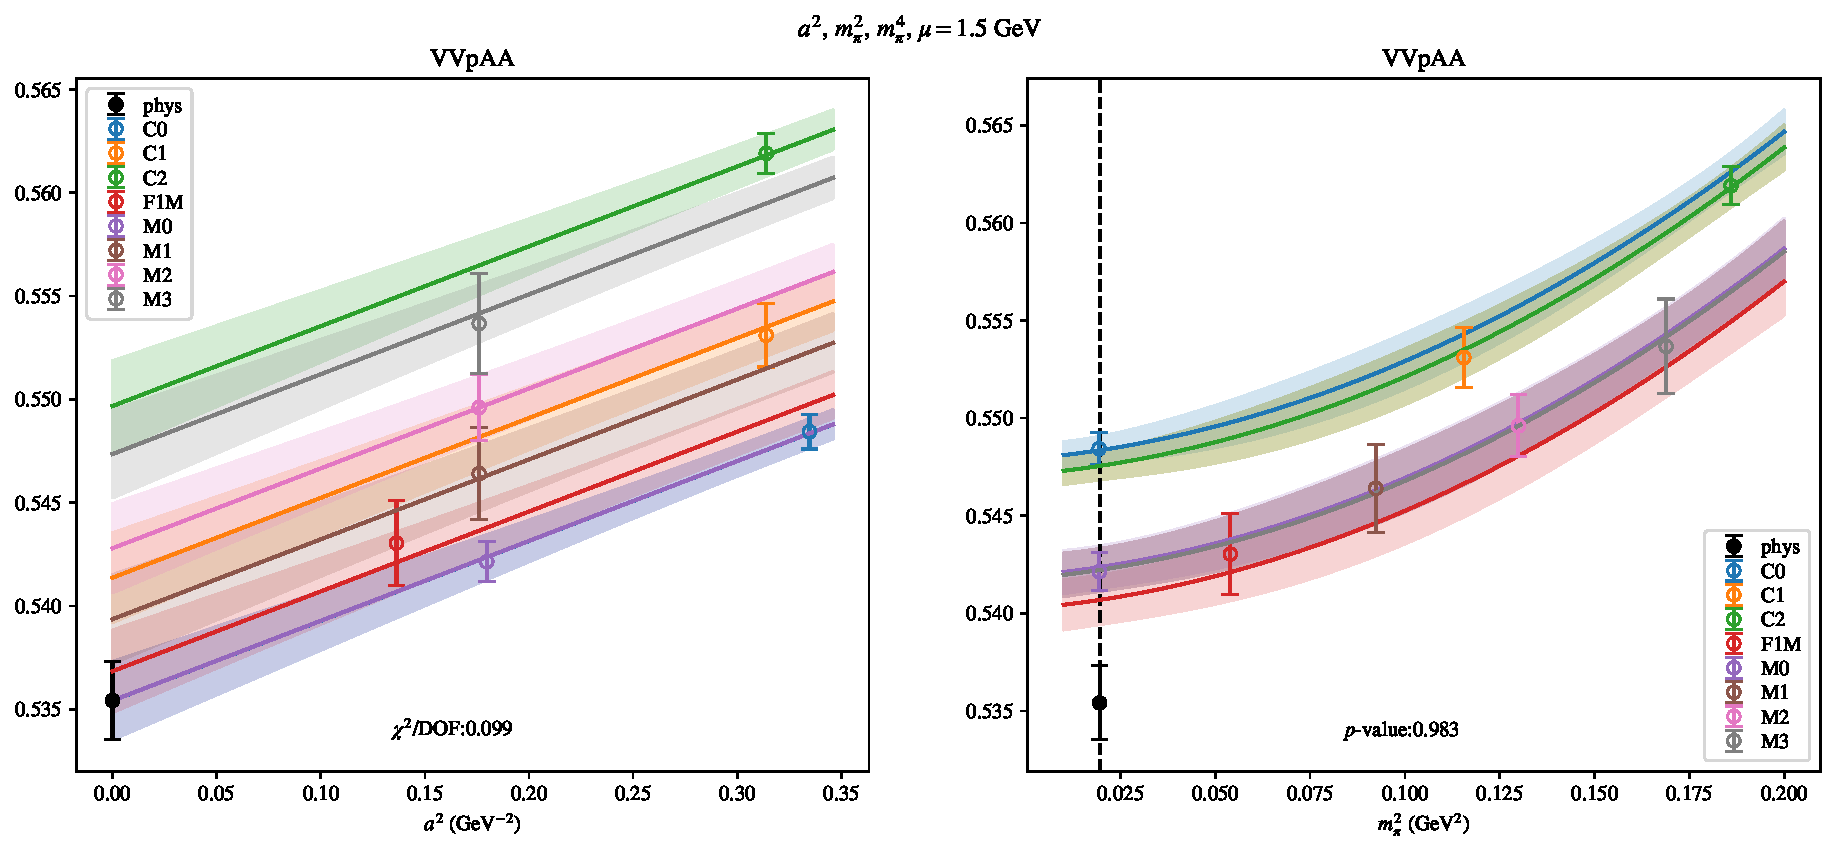
\includepdf[link, pages=-]{VVpAA/NPR/a2m2m4_15.pdf}
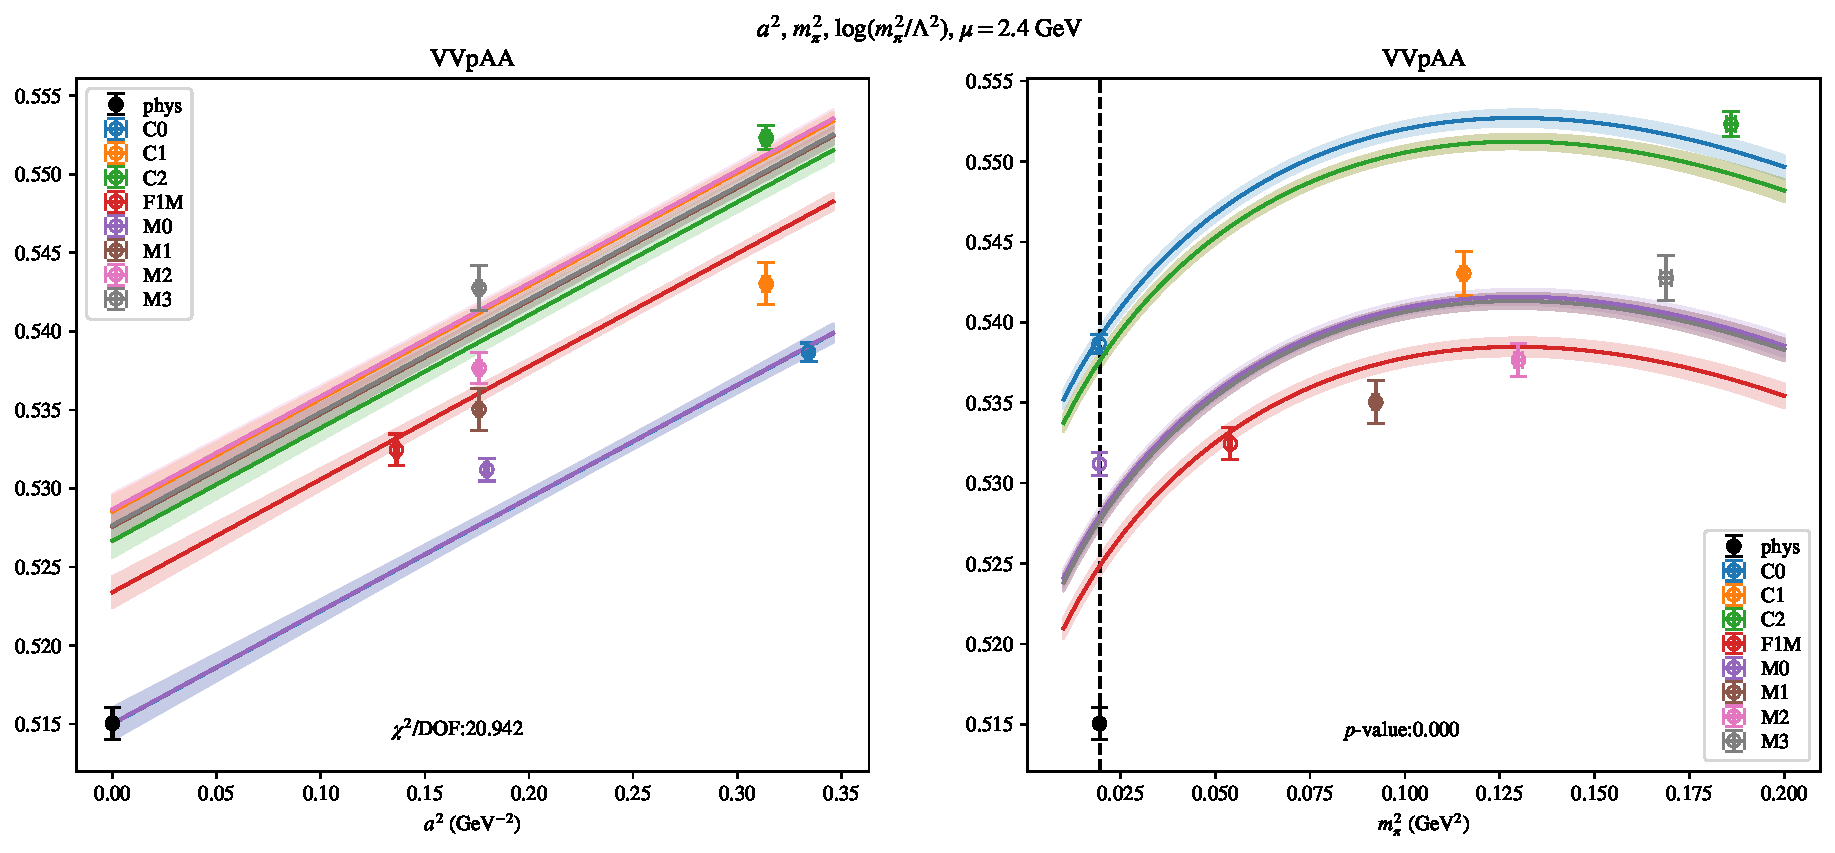
\includepdf[link, pages=-]{VVpAA/NPR/a2m2logm2_24.pdf}
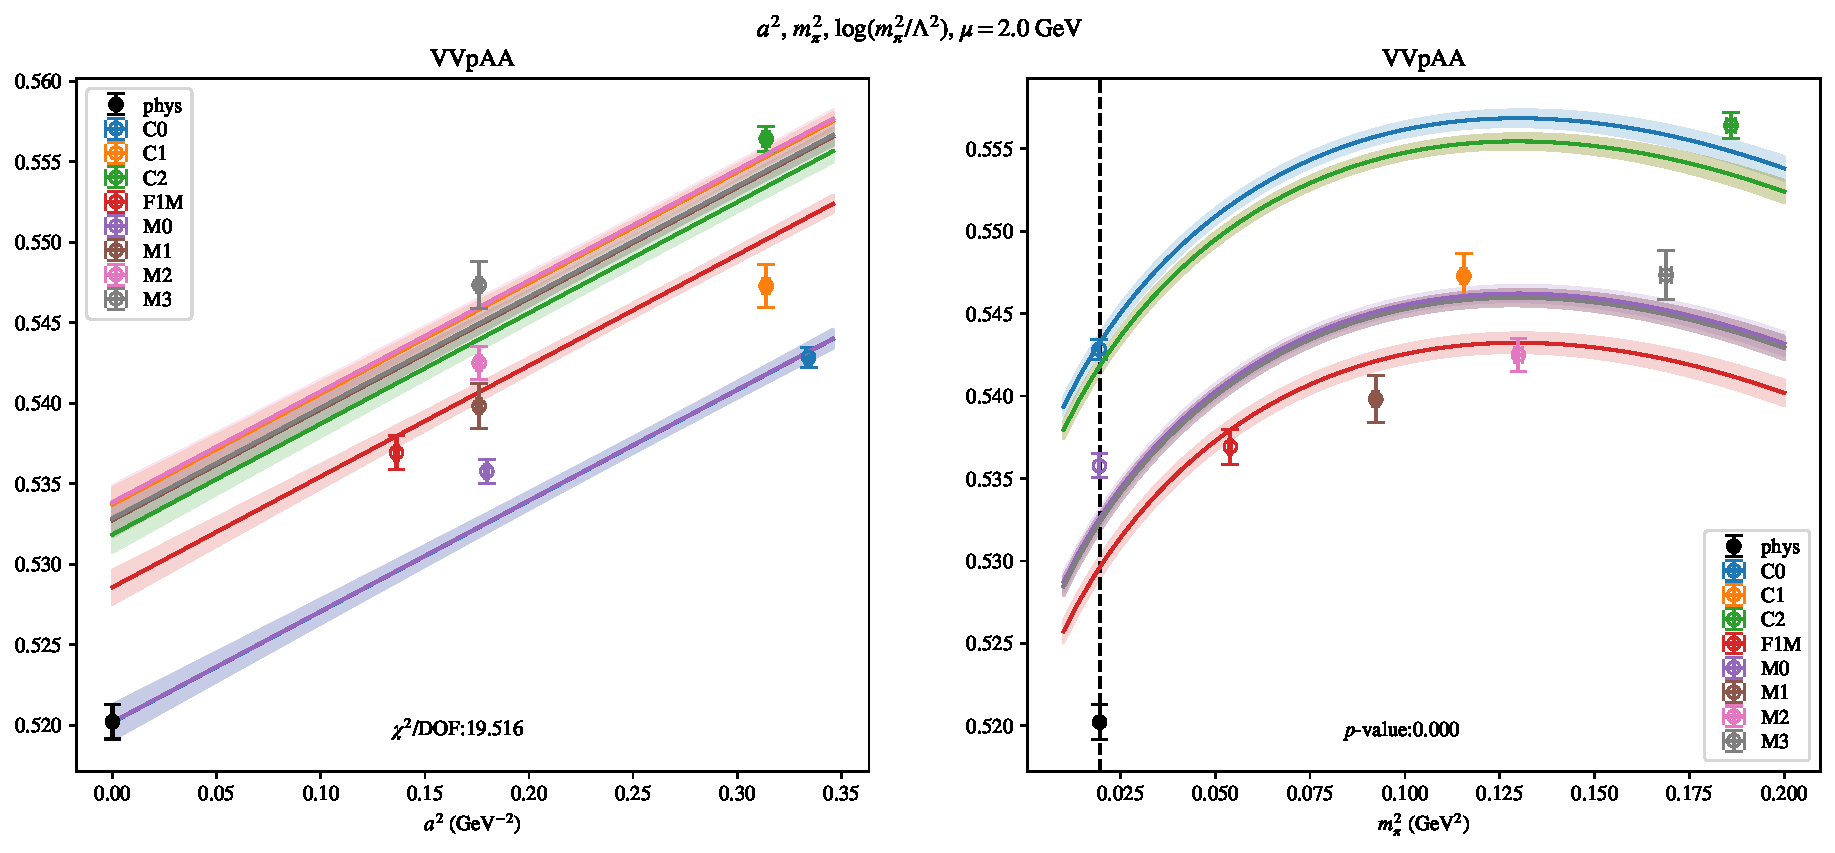
\includepdf[link, pages=-]{VVpAA/NPR/a2m2logm2_20.pdf}
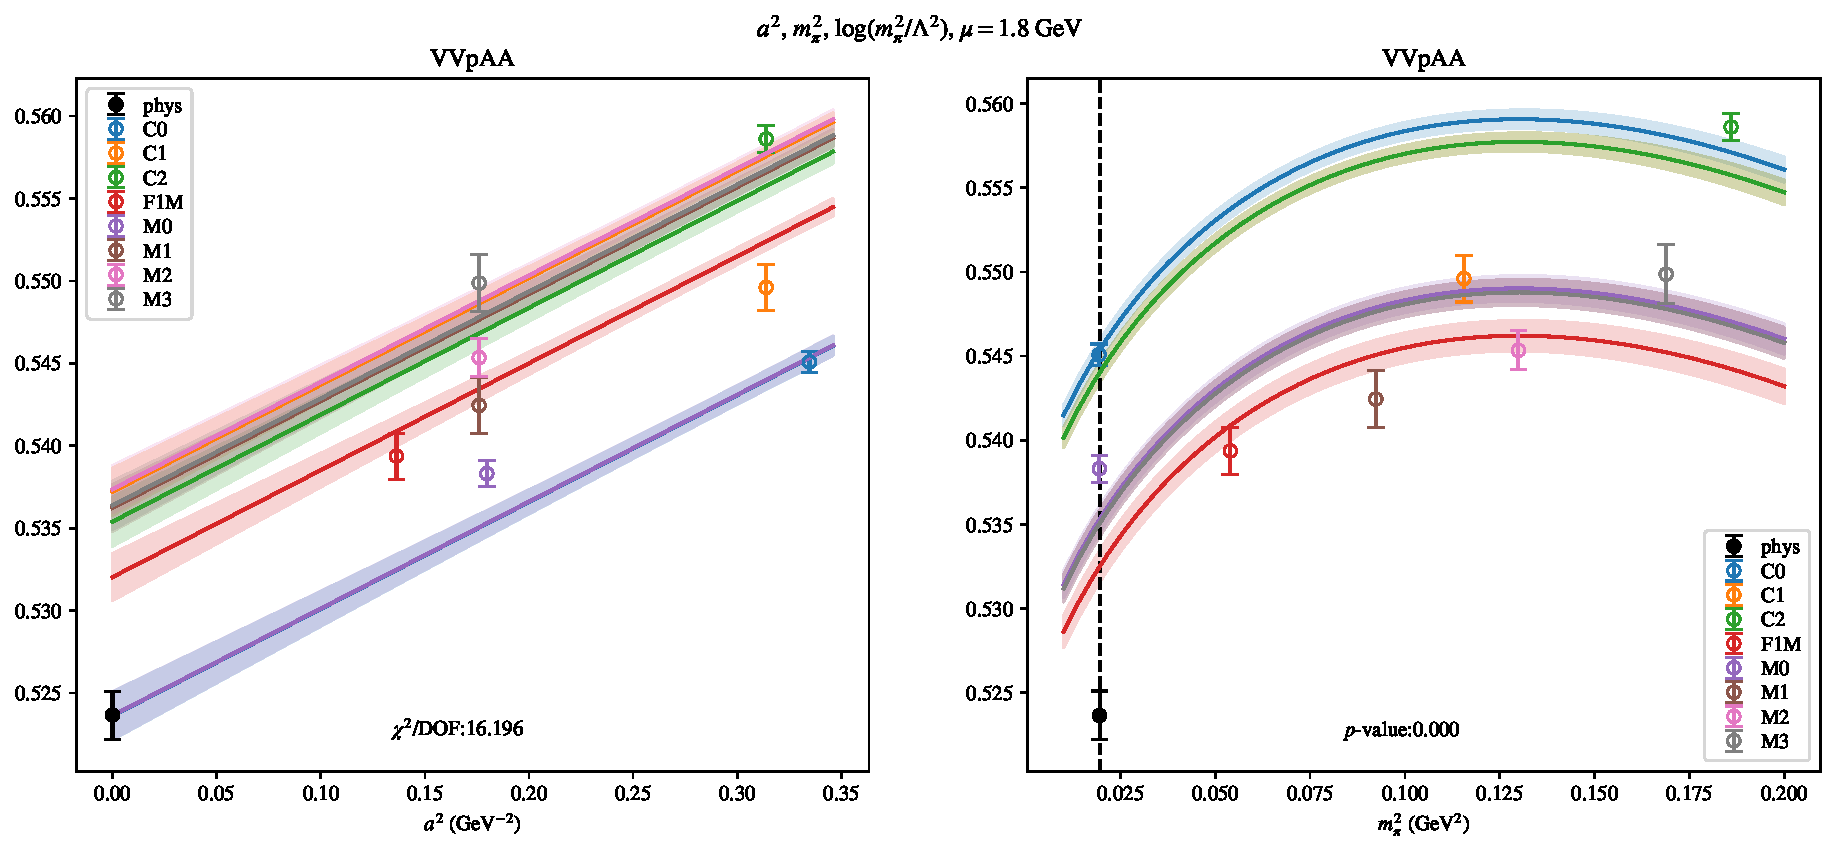
\includepdf[link, pages=-]{VVpAA/NPR/a2m2logm2_18.pdf}
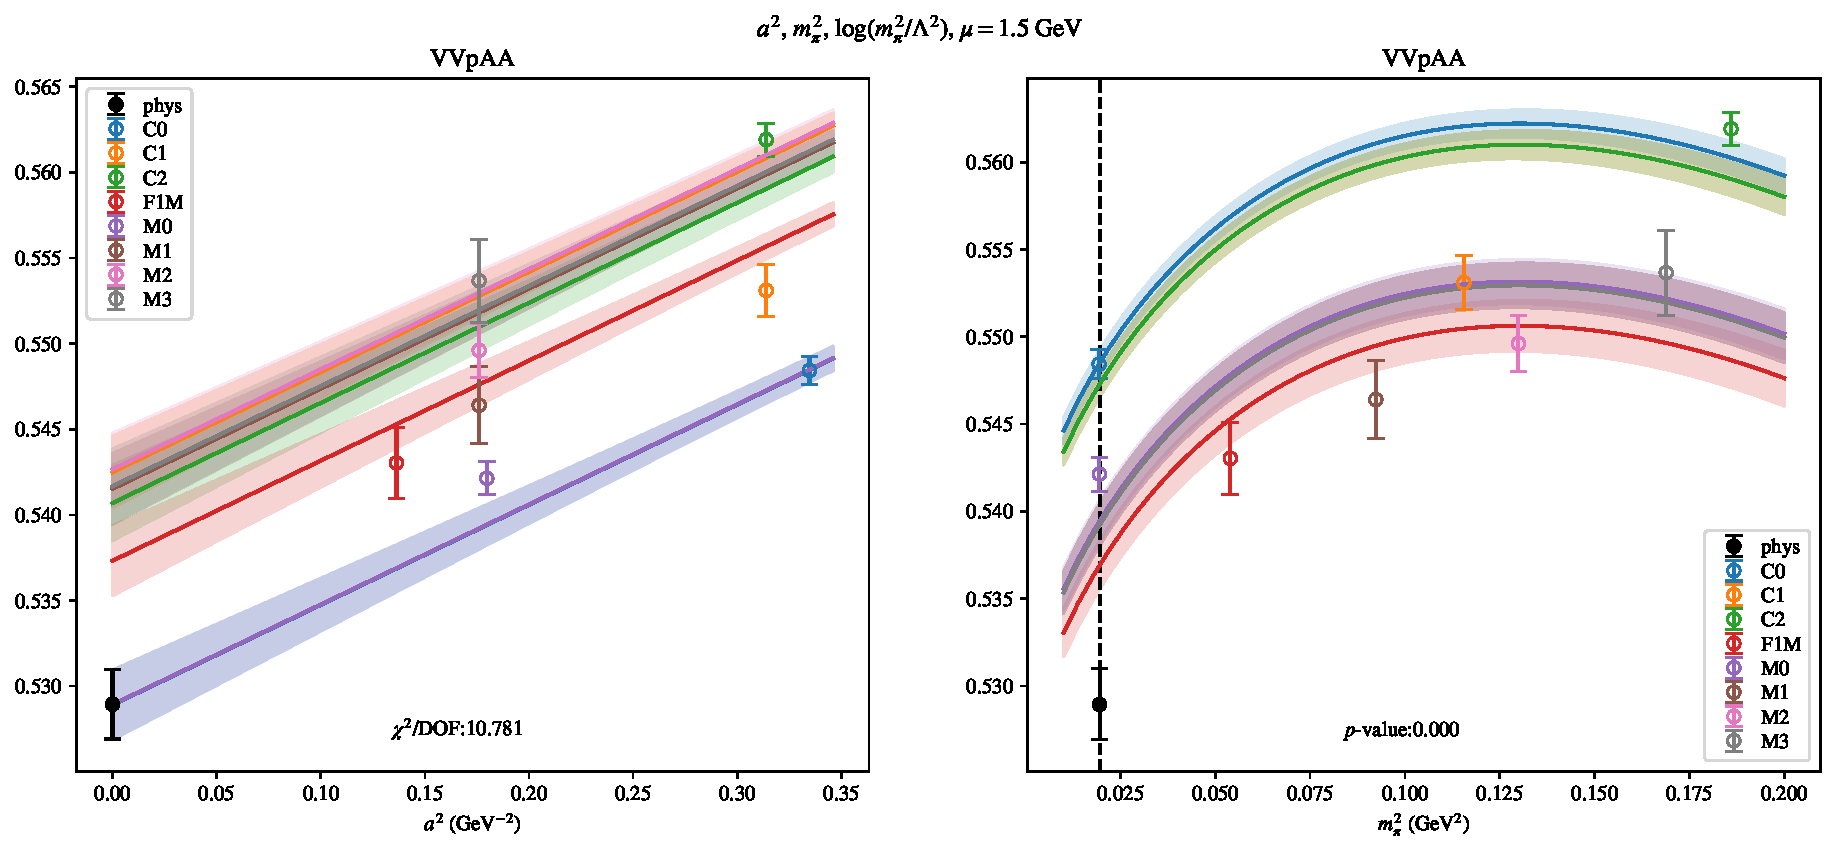
\includepdf[link, pages=-]{VVpAA/NPR/a2m2logm2_15.pdf}
\clearpage
\section{$B_2$}
\begin{table}[h!]
\begin{center}
\begin{tabular}{|c|c|c|c|c|c|}
\hline
$\mu$ (GeV) & $a^2$, $m_\pi^2$& $a^2$, $m_\pi^2$ (no C)& $a^2$, $a^4$, $m_\pi^2$& $a^2$, $m_\pi^2$, $m_\pi^4$& $a^2$, $m_\pi^2$, $\log(m_\pi^2/\Lambda^2)$\\
\hline
2.4& \hyperlink{VVmAA/NPR/a2m2_24.pdf.1}{\textbf{1.9828(25)}: 8.464 (0.0)} & \hyperlink{VVmAA/NPR/a2m2noC_24.pdf.1}{\textbf{2.070(13)}: 0.597 (0.55)} & \hyperlink{VVmAA/NPR/a2a4m2_24.pdf.1}{\textbf{2.122(21)}: 0.86 (0.487)} & \hyperlink{VVmAA/NPR/a2m2m4_24.pdf.1}{\textbf{1.9810(25)}: 9.602 (0.0)} & \hyperlink{VVmAA/NPR/a2m2logm2_24.pdf.1}{\textbf{1.9481(24)}: 9.563 (0.0)}\\
2.0& \hyperlink{VVmAA/NPR/a2m2_20.pdf.1}{\textbf{2.3714(31)}: 8.812 (0.0)} & \hyperlink{VVmAA/NPR/a2m2noC_20.pdf.1}{\textbf{2.470(16)}: 0.354 (0.702)} & \hyperlink{VVmAA/NPR/a2a4m2_20.pdf.1}{\textbf{2.555(26)}: 0.418 (0.796)} & \hyperlink{VVmAA/NPR/a2m2m4_20.pdf.1}{\textbf{2.3688(31)}: 9.437 (0.0)} & \hyperlink{VVmAA/NPR/a2m2logm2_20.pdf.1}{\textbf{2.3307(31)}: 8.041 (0.0)}\\
1.8& \hyperlink{VVmAA/NPR/a2m2_18.pdf.1}{\textbf{2.5968(42)}: 8.923 (0.0)} & \hyperlink{VVmAA/NPR/a2m2noC_18.pdf.1}{\textbf{2.692(19)}: 0.993 (0.371)} & \hyperlink{VVmAA/NPR/a2a4m2_18.pdf.1}{\textbf{2.821(31)}: 2.489 (0.041)} & \hyperlink{VVmAA/NPR/a2m2m4_18.pdf.1}{\textbf{2.5945(40)}: 10.51 (0.0)} & \hyperlink{VVmAA/NPR/a2m2logm2_18.pdf.1}{\textbf{2.5516(41)}: 9.637 (0.0)}\\
1.5& \hyperlink{VVmAA/NPR/a2m2_15.pdf.1}{\textbf{2.9376(65)}: 9.386 (0.0)} & \hyperlink{VVmAA/NPR/a2m2noC_15.pdf.1}{\textbf{3.026(26)}: 1.469 (0.23)} & \hyperlink{VVmAA/NPR/a2a4m2_15.pdf.1}{\textbf{3.232(43)}: 5.497 (0.0)} & \hyperlink{VVmAA/NPR/a2m2m4_15.pdf.1}{\textbf{2.9360(58)}: 11.616 (0.0)} & \hyperlink{VVmAA/NPR/a2m2logm2_15.pdf.1}{\textbf{2.8854(64)}: 10.9 (0.0)}\\
\hline
\end{tabular}
\caption{Physical point value from chiral and continuum extrapolation at renormalisation scale $\mu$. Entries are \textbf{value(error)}: $\chi^2/\text{DOF}$ ($p$-value).}
\end{center}
\end{table}
\begin{table}[h!]
\begin{center}
\begin{tabular}{|c c|c|c|c|c|c|}
\hline
$\mu$ (GeV) &  & $a^2$, $m_\pi^2$& $a^2$, $m_\pi^2$ (no C)& $a^2$, $a^4$, $m_\pi^2$& $a^2$, $m_\pi^2$, $m_\pi^4$& $a^2$, $m_\pi^2$, $\log(m_\pi^2/\Lambda^2)$\\
\hline
\multirow{2}{0.5in}{2.4} & $\alpha$ & -0.578(37)& -0.79(32)& -1.12(78)& -0.576(39)& -0.574(38)\\
 & $\beta$ & 0.00087(10)& 0.00090(18)& 0.001053(99)& 0.00198(55)& -0.0038(10)\\
\hline
\multirow{2}{0.5in}{2.0} & $\alpha$ & -0.681(36)& -0.88(31)& -1.27(76)& -0.679(36)& -0.679(36)\\
 & $\beta$ & 0.00112(12)& 0.00147(23)& 0.00129(12)& 0.00267(59)& -0.0036(12)\\
\hline
\multirow{2}{0.5in}{1.8} & $\alpha$ & -0.703(37)& -0.89(33)& -1.35(80)& -0.701(37)& -0.701(38)\\
 & $\beta$ & 0.00087(13)& 0.00166(24)& 0.00109(13)& 0.00199(61)& -0.0039(13)\\
\hline
\multirow{2}{0.5in}{1.5} & $\alpha$ & -0.733(40)& -0.89(38)& -1.47(91)& -0.732(38)& -0.730(40)\\
 & $\beta$ & 0.00056(14)& 0.00188(26)& 0.00086(14)& 0.00115(67)& -0.0042(14)\\
\hline
\end{tabular}
\caption{Fit values of coefficients in $B = B_0(1 + \mathbf{\alpha} a^2 + \mathbf{\beta} \frac{m_\pi^2}{f_\pi^2} + \ldots)$.}
\end{center}
\end{table}
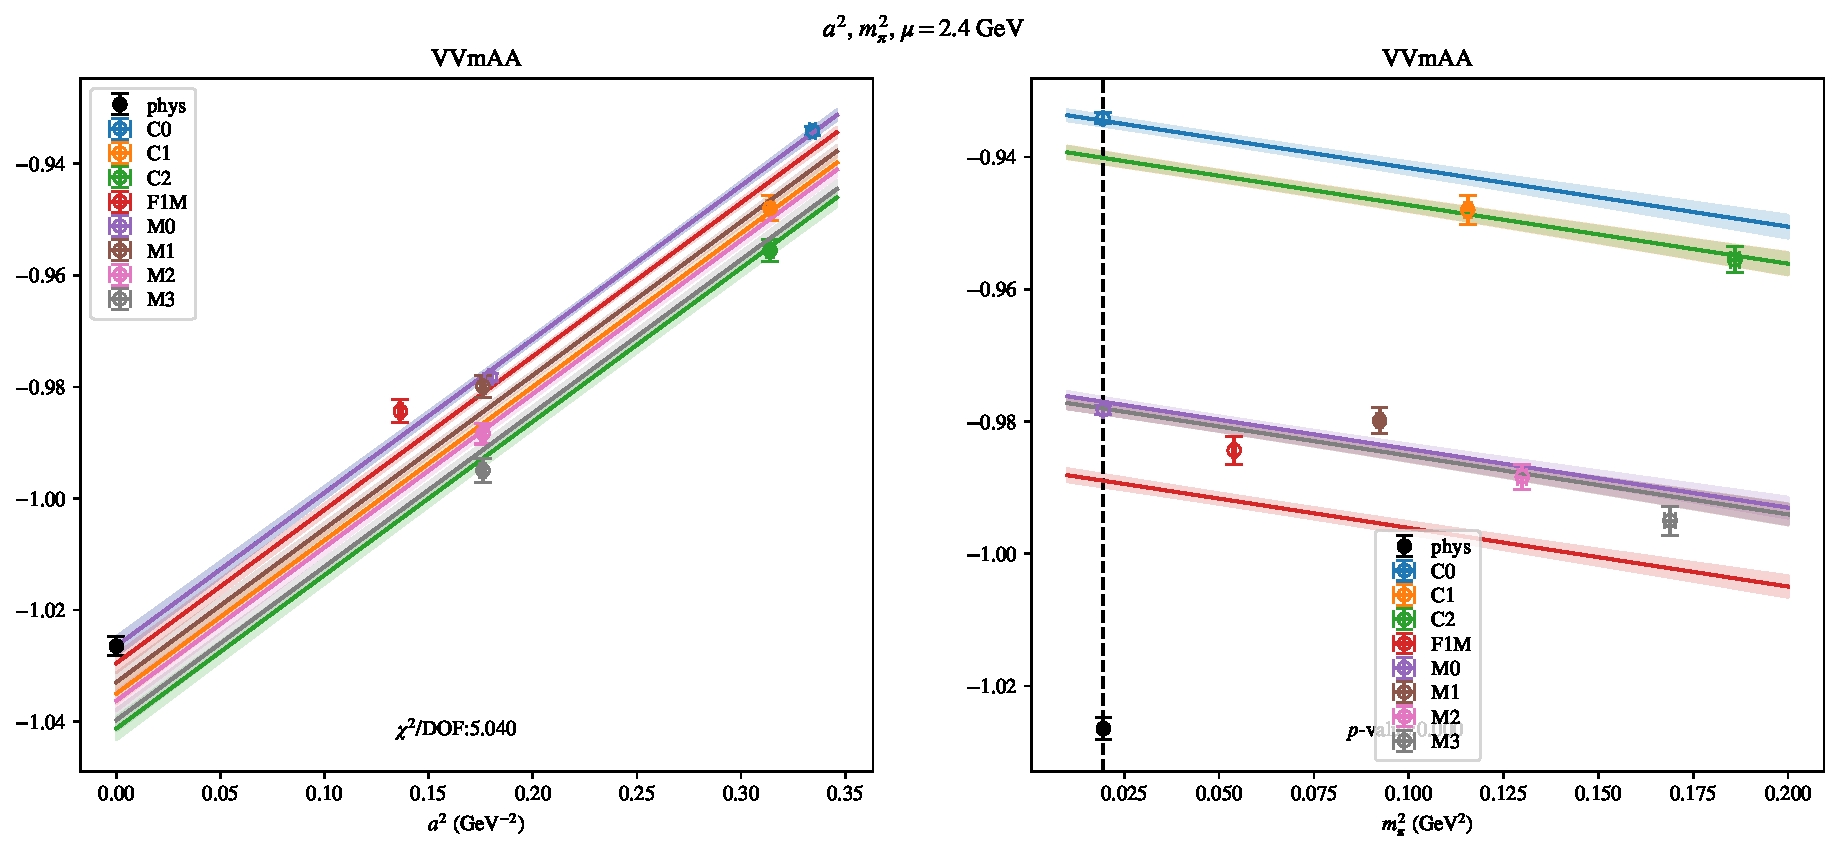
\includepdf[link, pages=-]{VVmAA/NPR/a2m2_24.pdf}
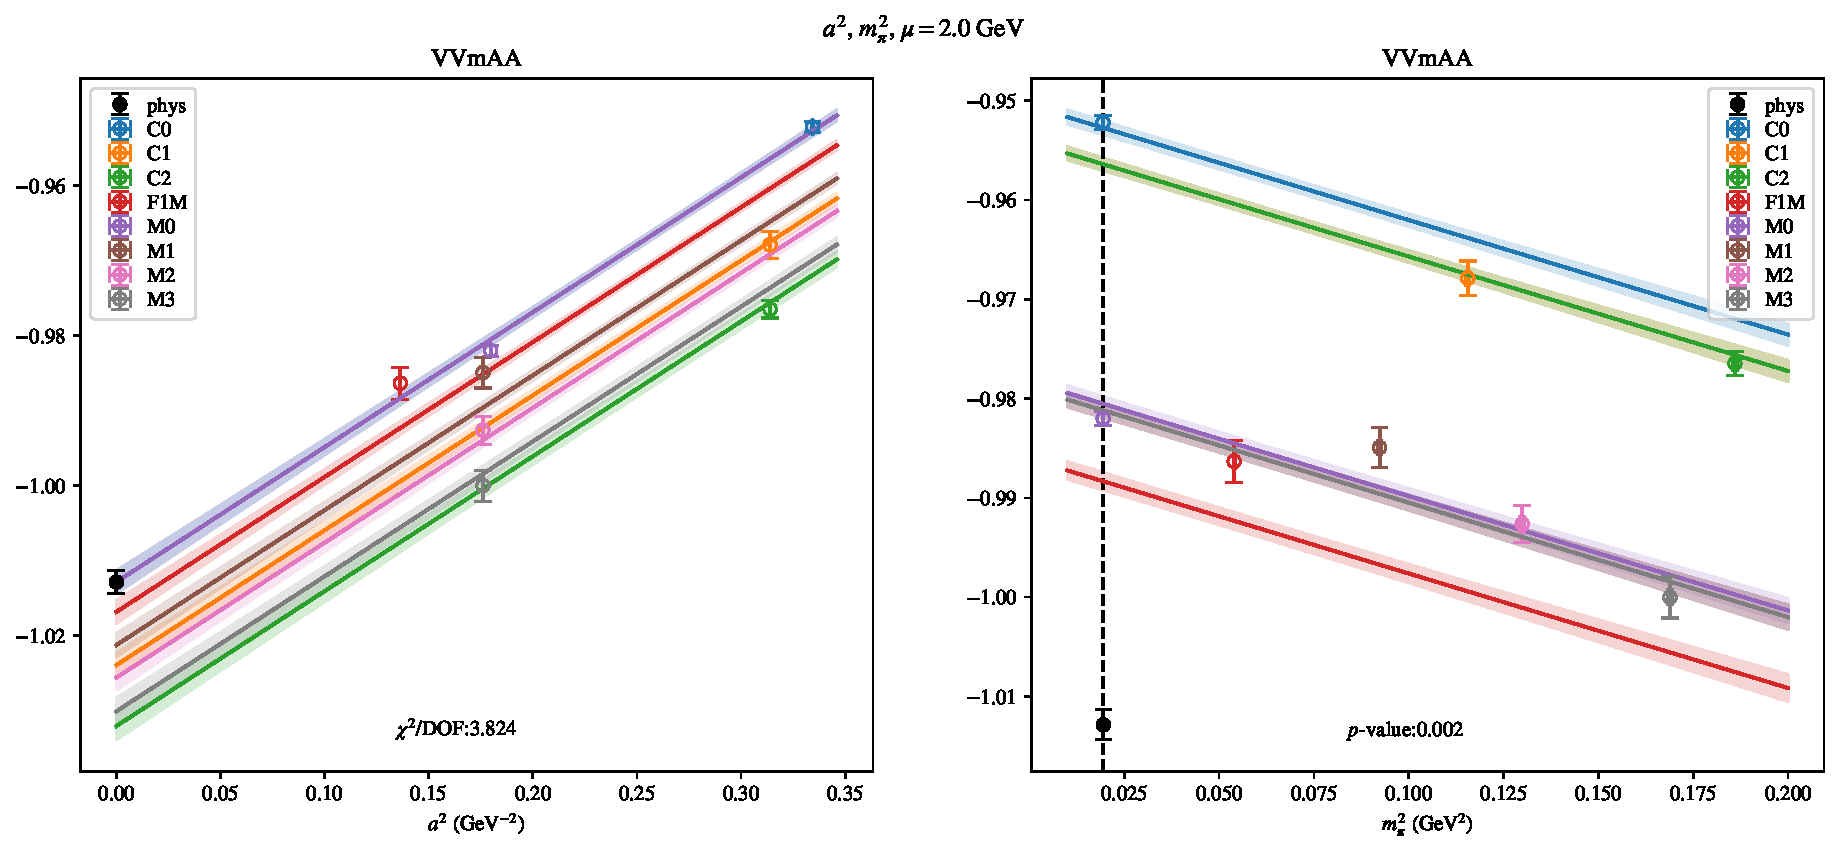
\includepdf[link, pages=-]{VVmAA/NPR/a2m2_20.pdf}
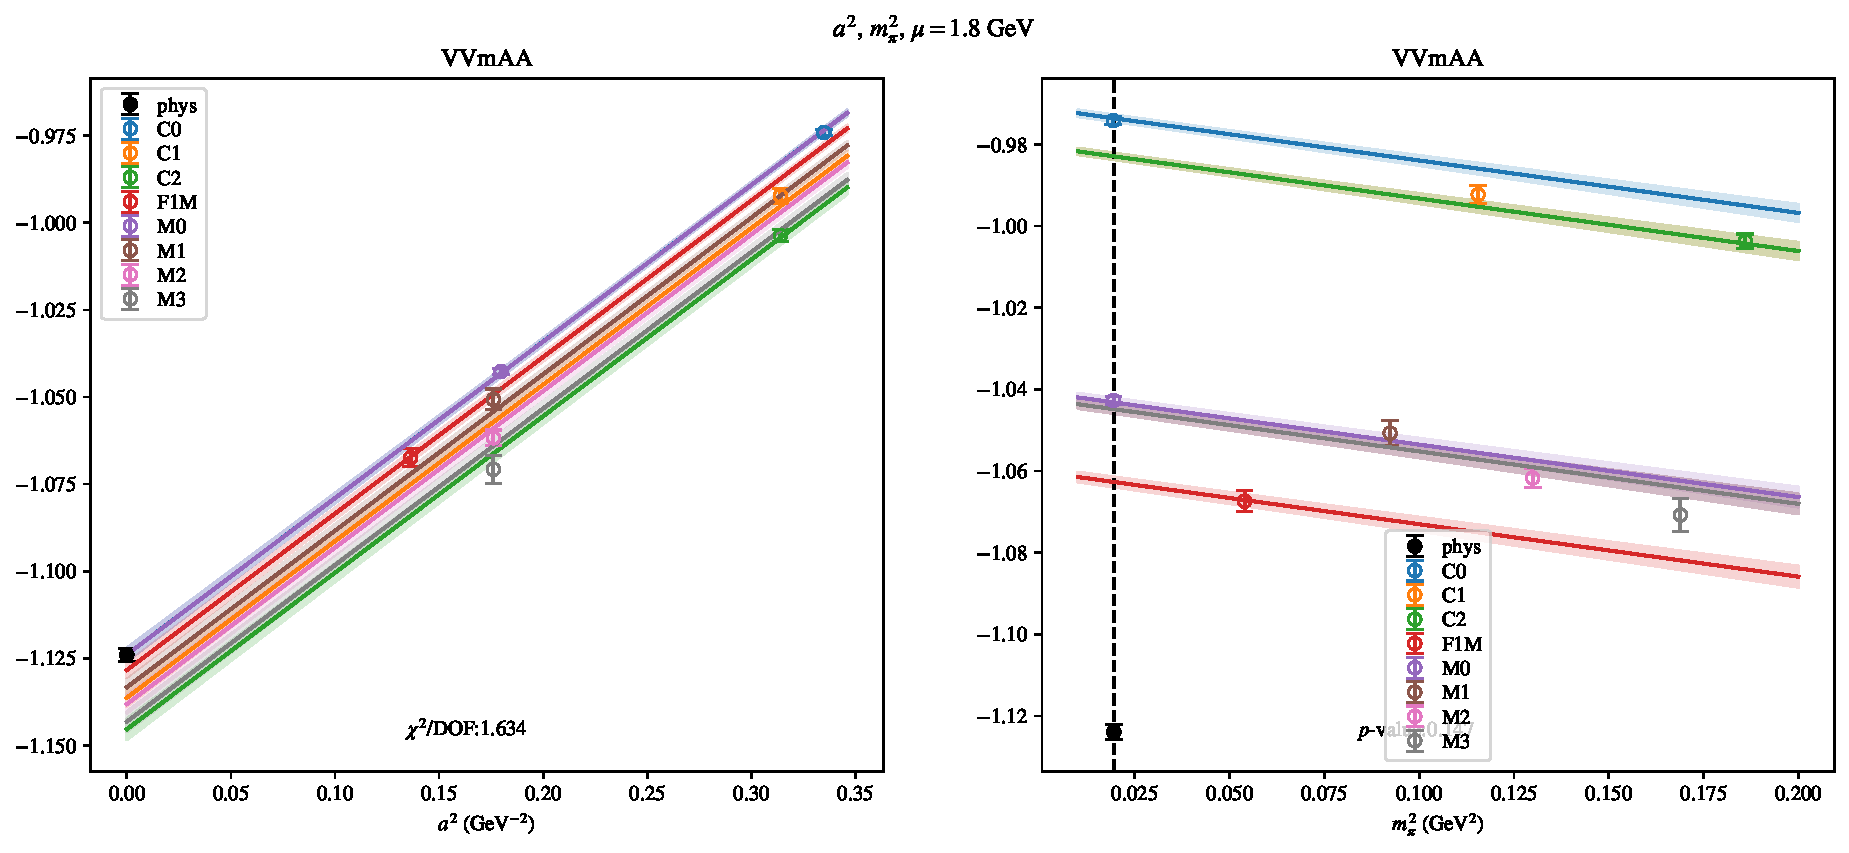
\includepdf[link, pages=-]{VVmAA/NPR/a2m2_18.pdf}
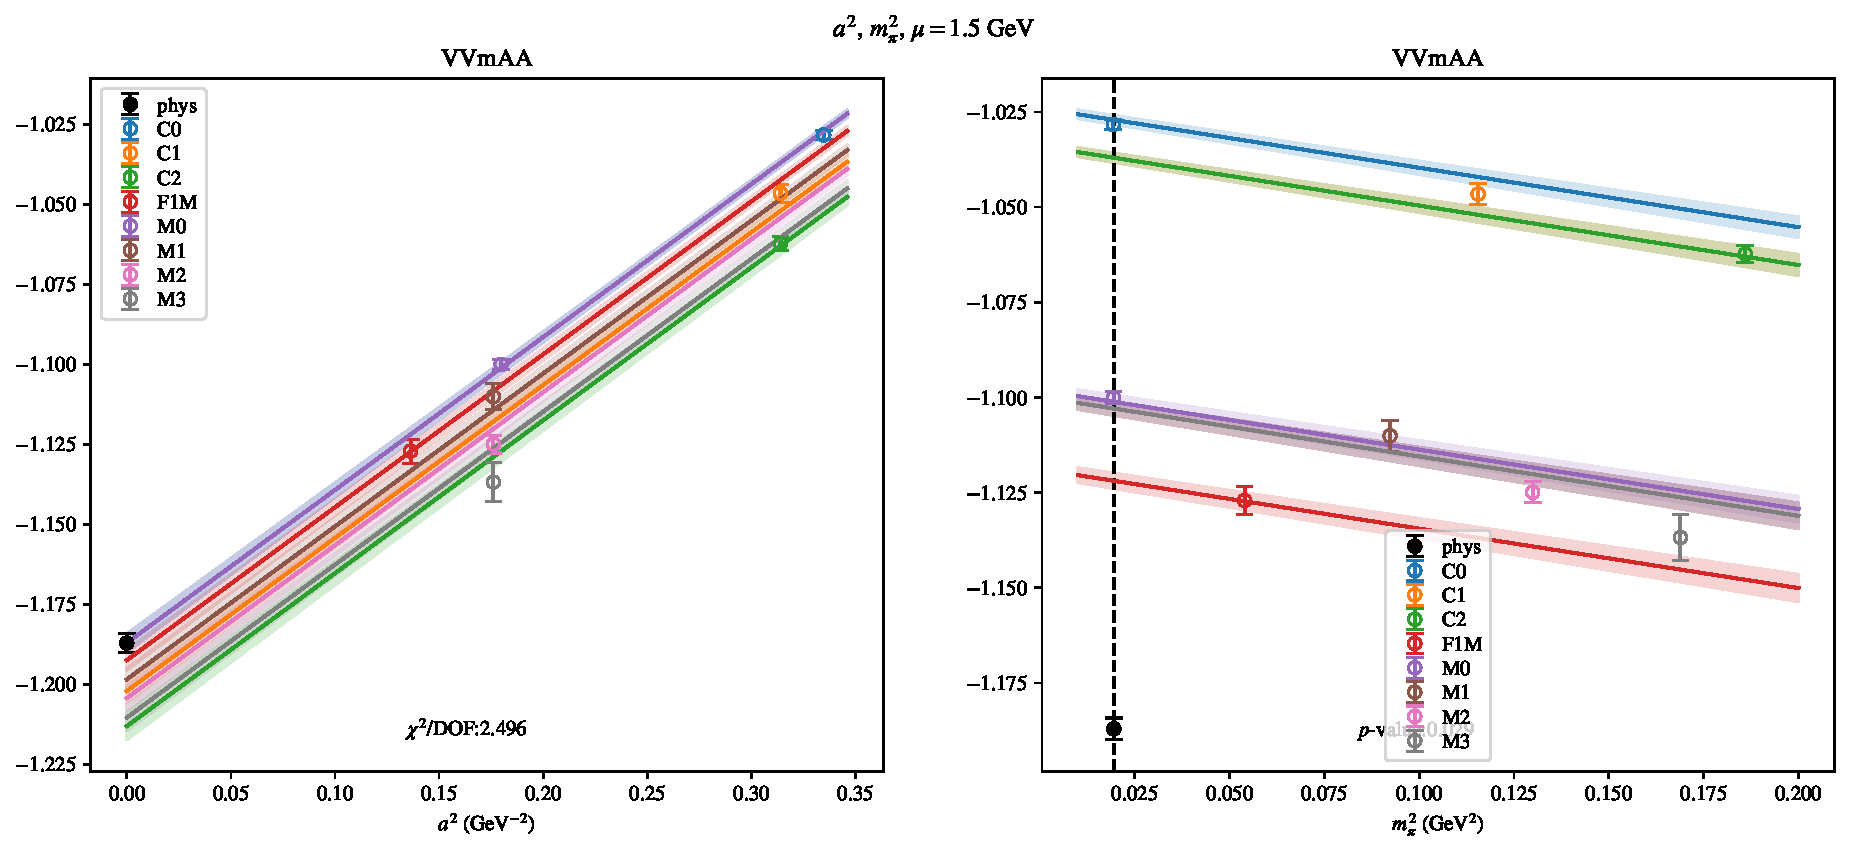
\includepdf[link, pages=-]{VVmAA/NPR/a2m2_15.pdf}
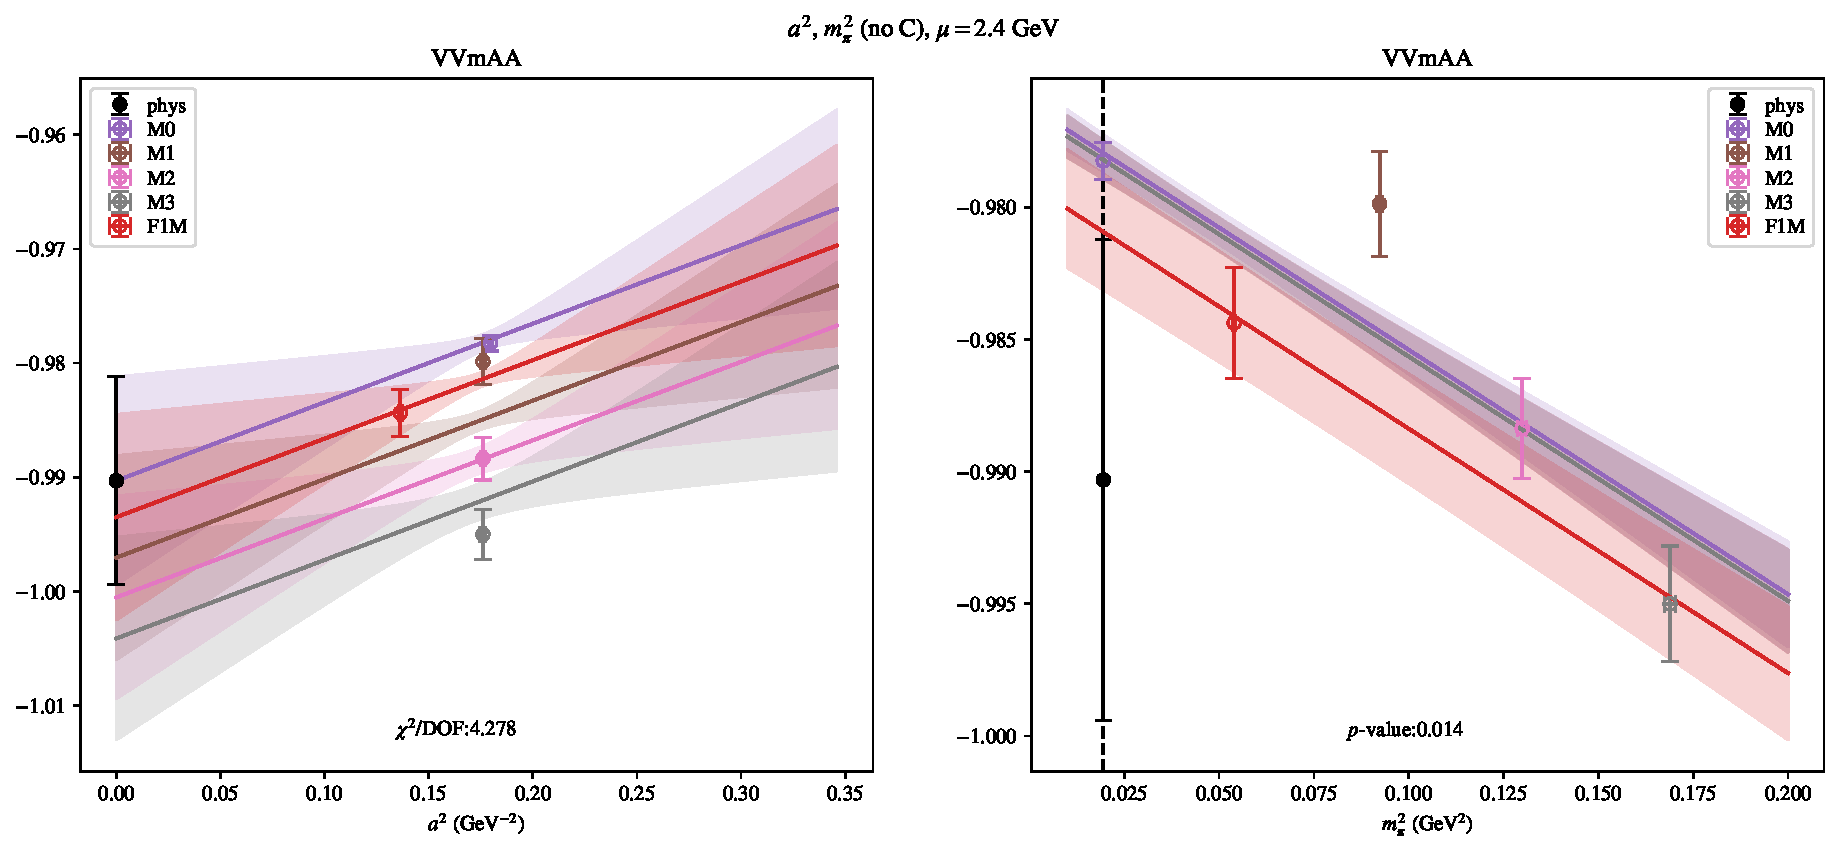
\includepdf[link, pages=-]{VVmAA/NPR/a2m2noC_24.pdf}
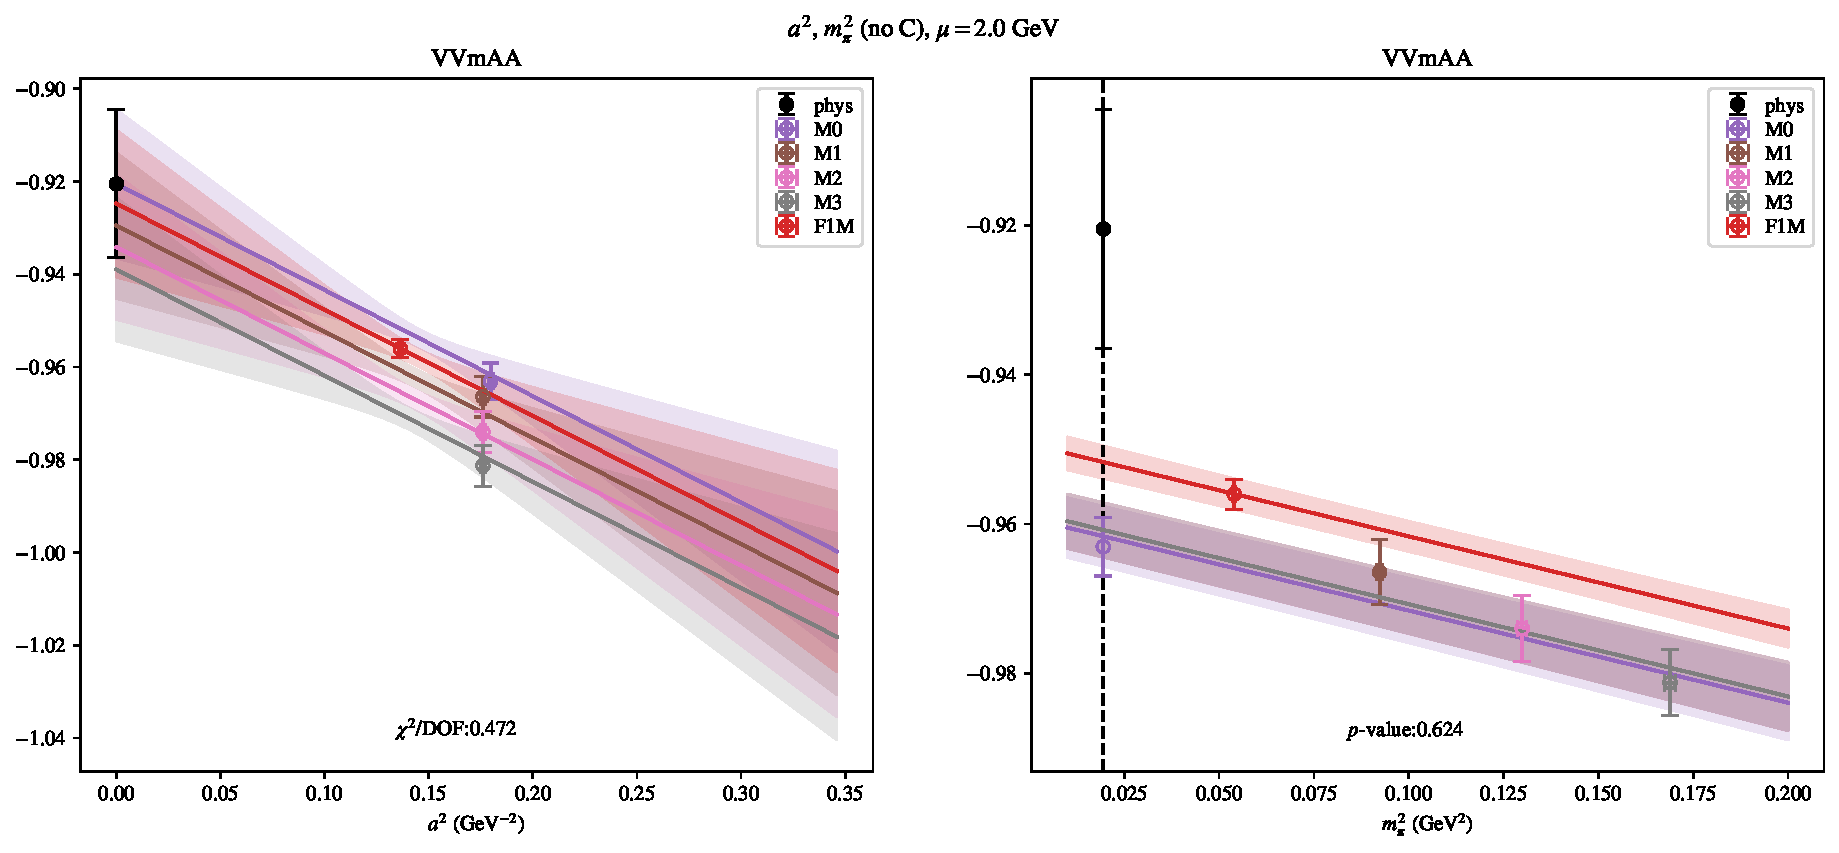
\includepdf[link, pages=-]{VVmAA/NPR/a2m2noC_20.pdf}
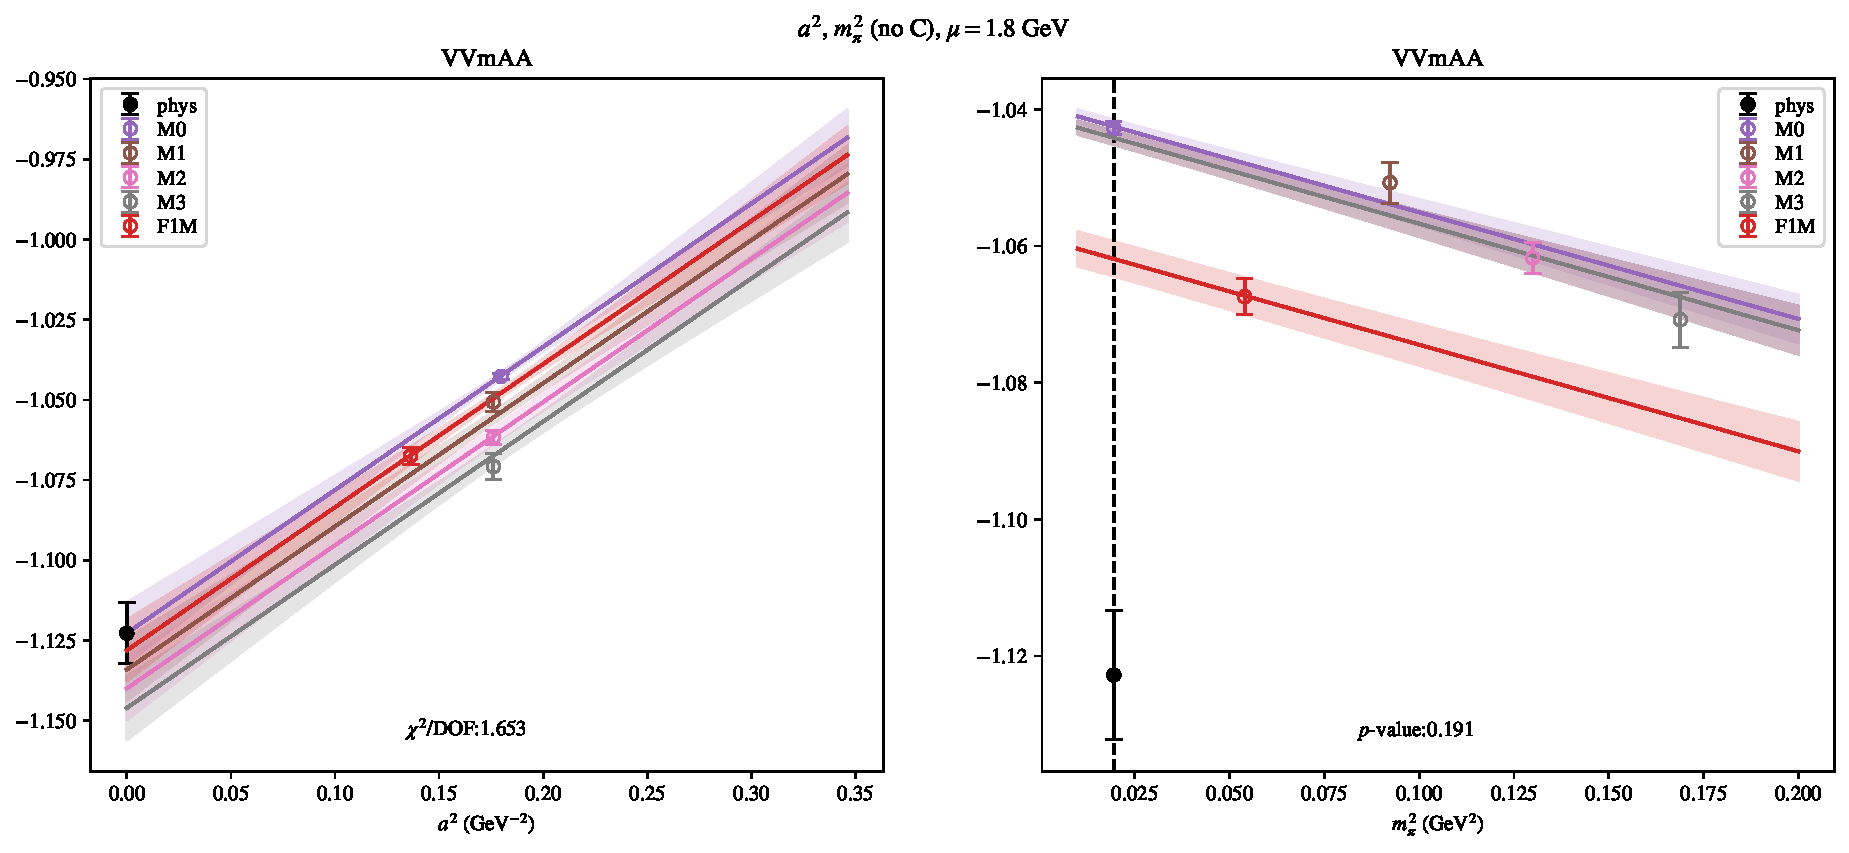
\includepdf[link, pages=-]{VVmAA/NPR/a2m2noC_18.pdf}
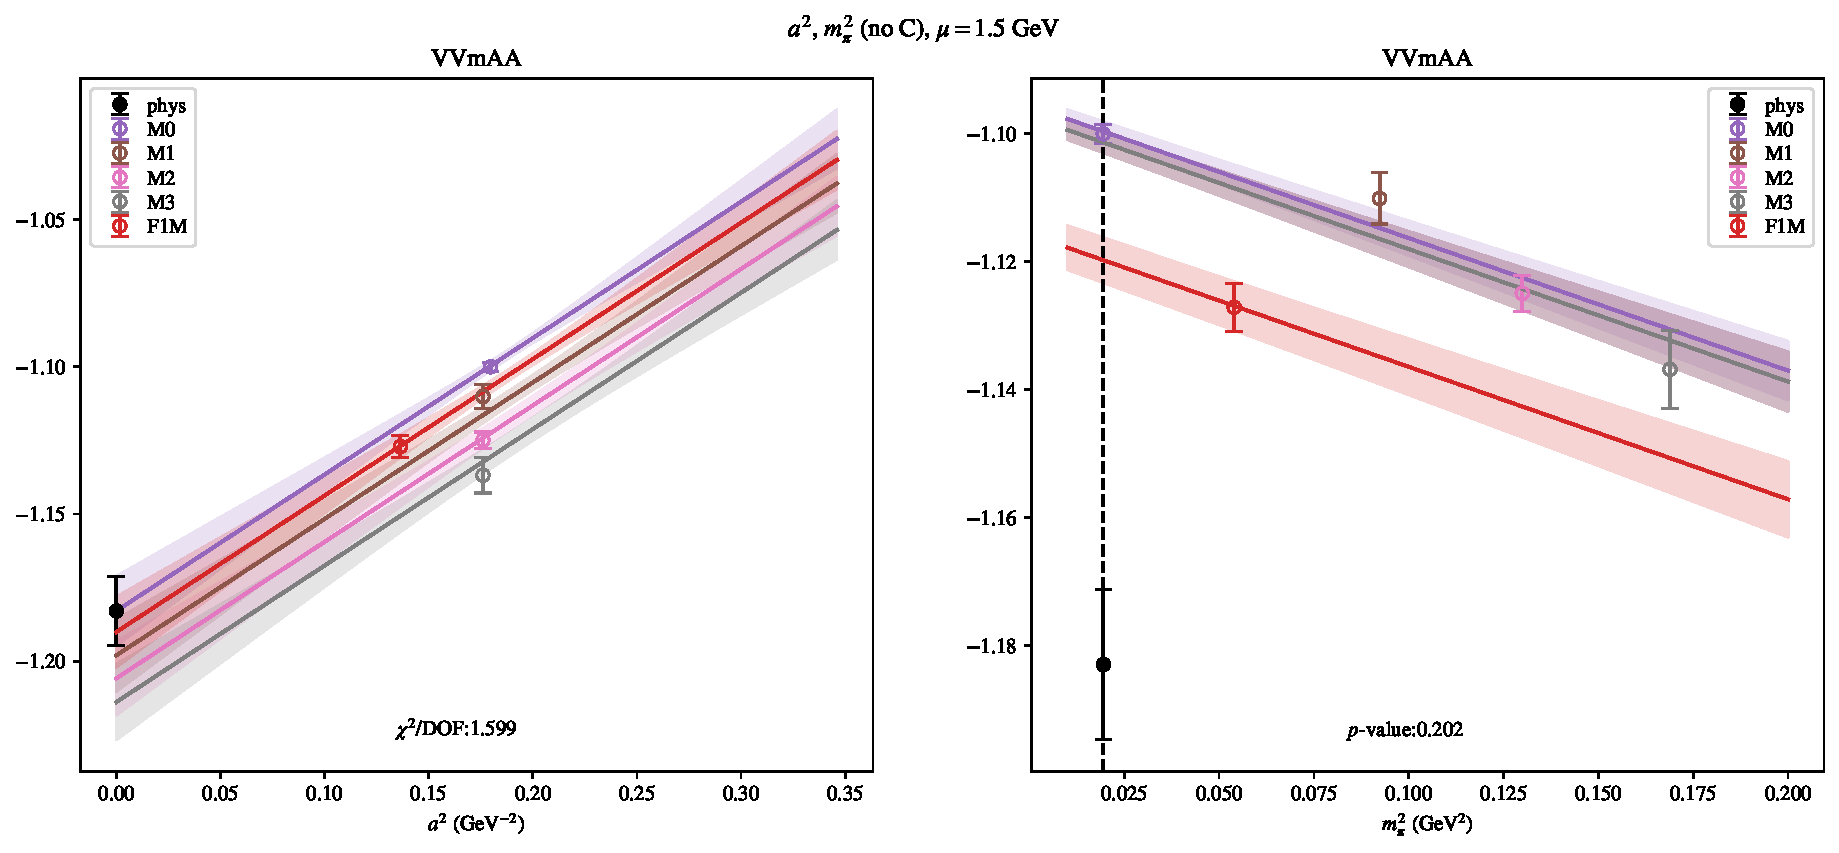
\includepdf[link, pages=-]{VVmAA/NPR/a2m2noC_15.pdf}
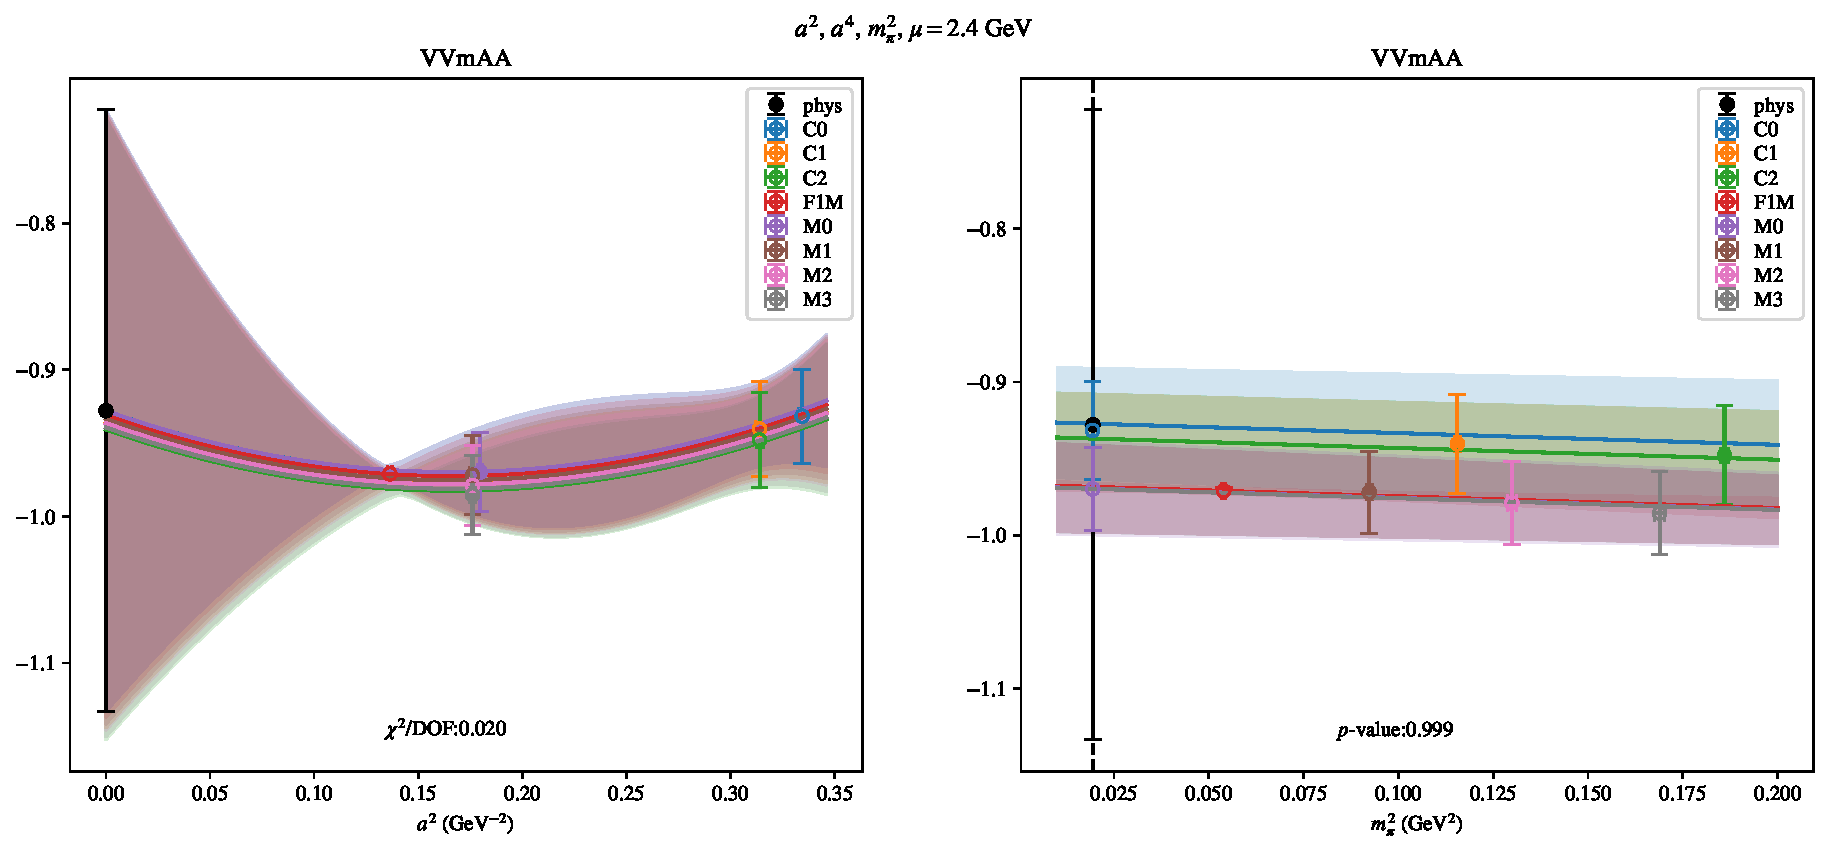
\includepdf[link, pages=-]{VVmAA/NPR/a2a4m2_24.pdf}
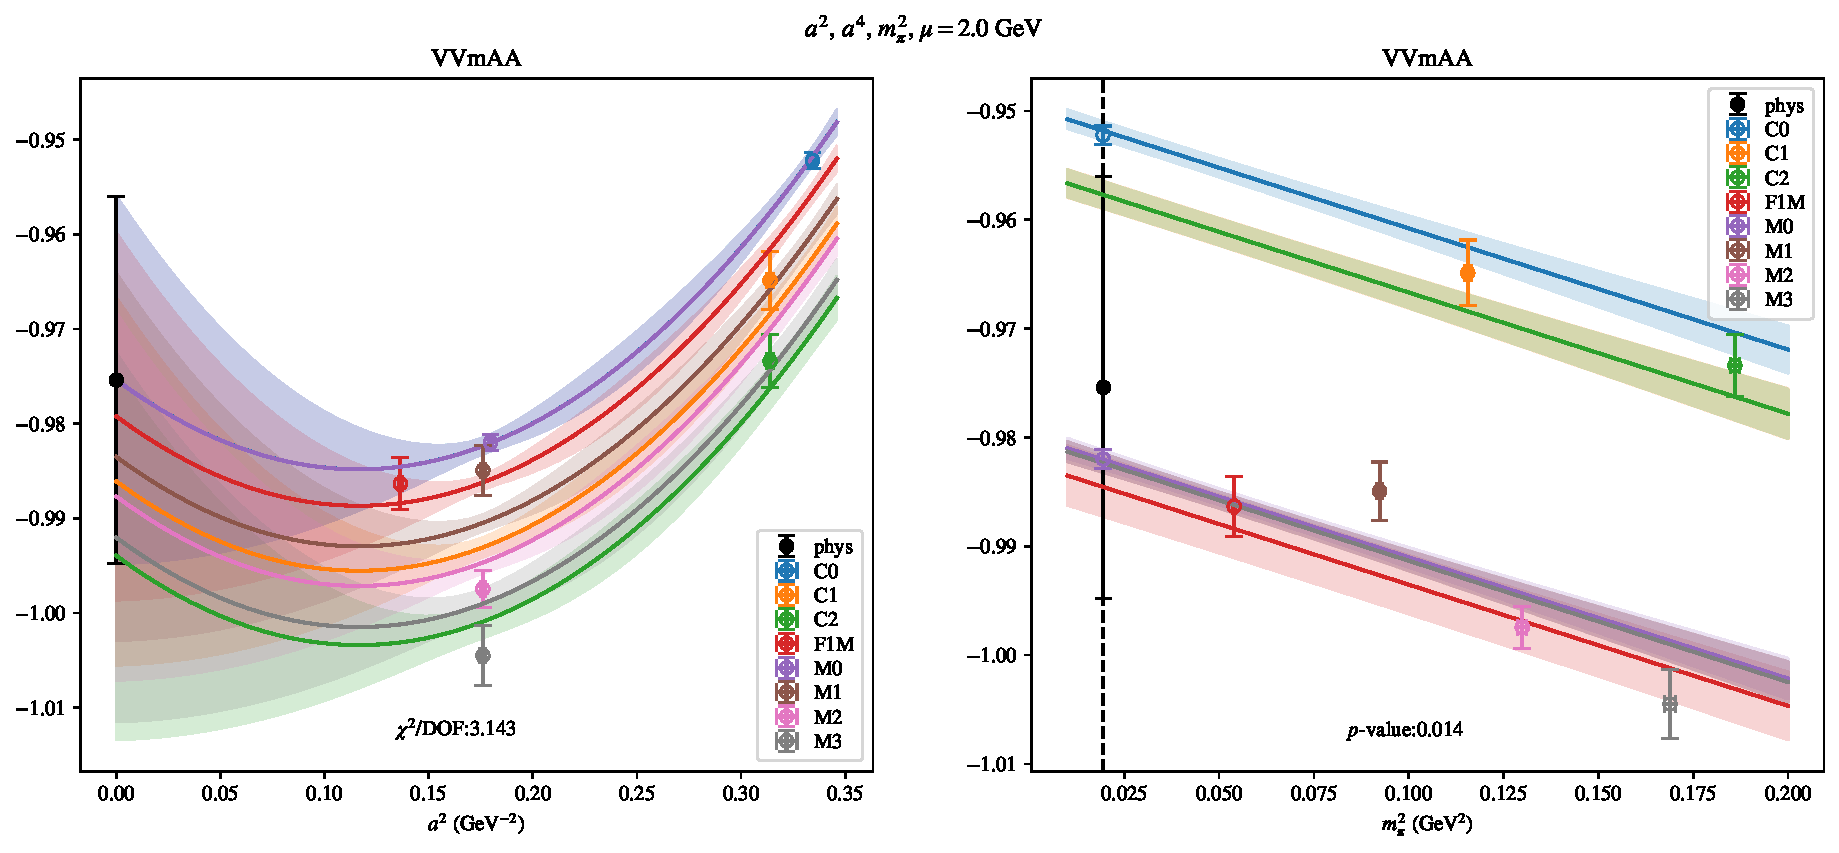
\includepdf[link, pages=-]{VVmAA/NPR/a2a4m2_20.pdf}
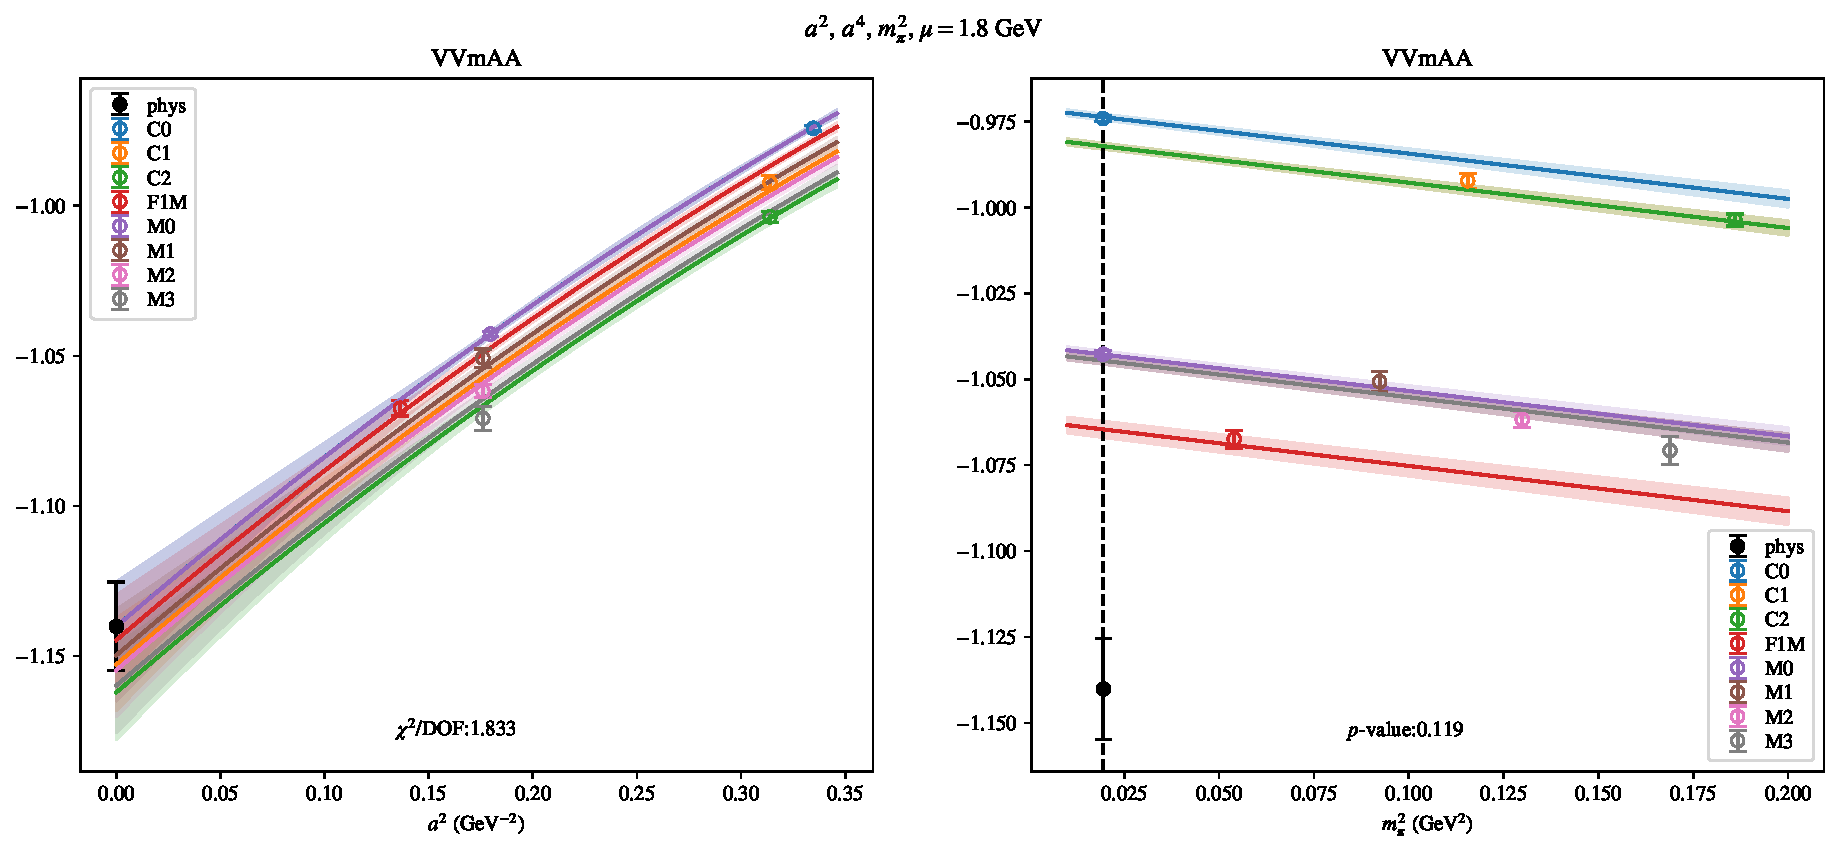
\includepdf[link, pages=-]{VVmAA/NPR/a2a4m2_18.pdf}
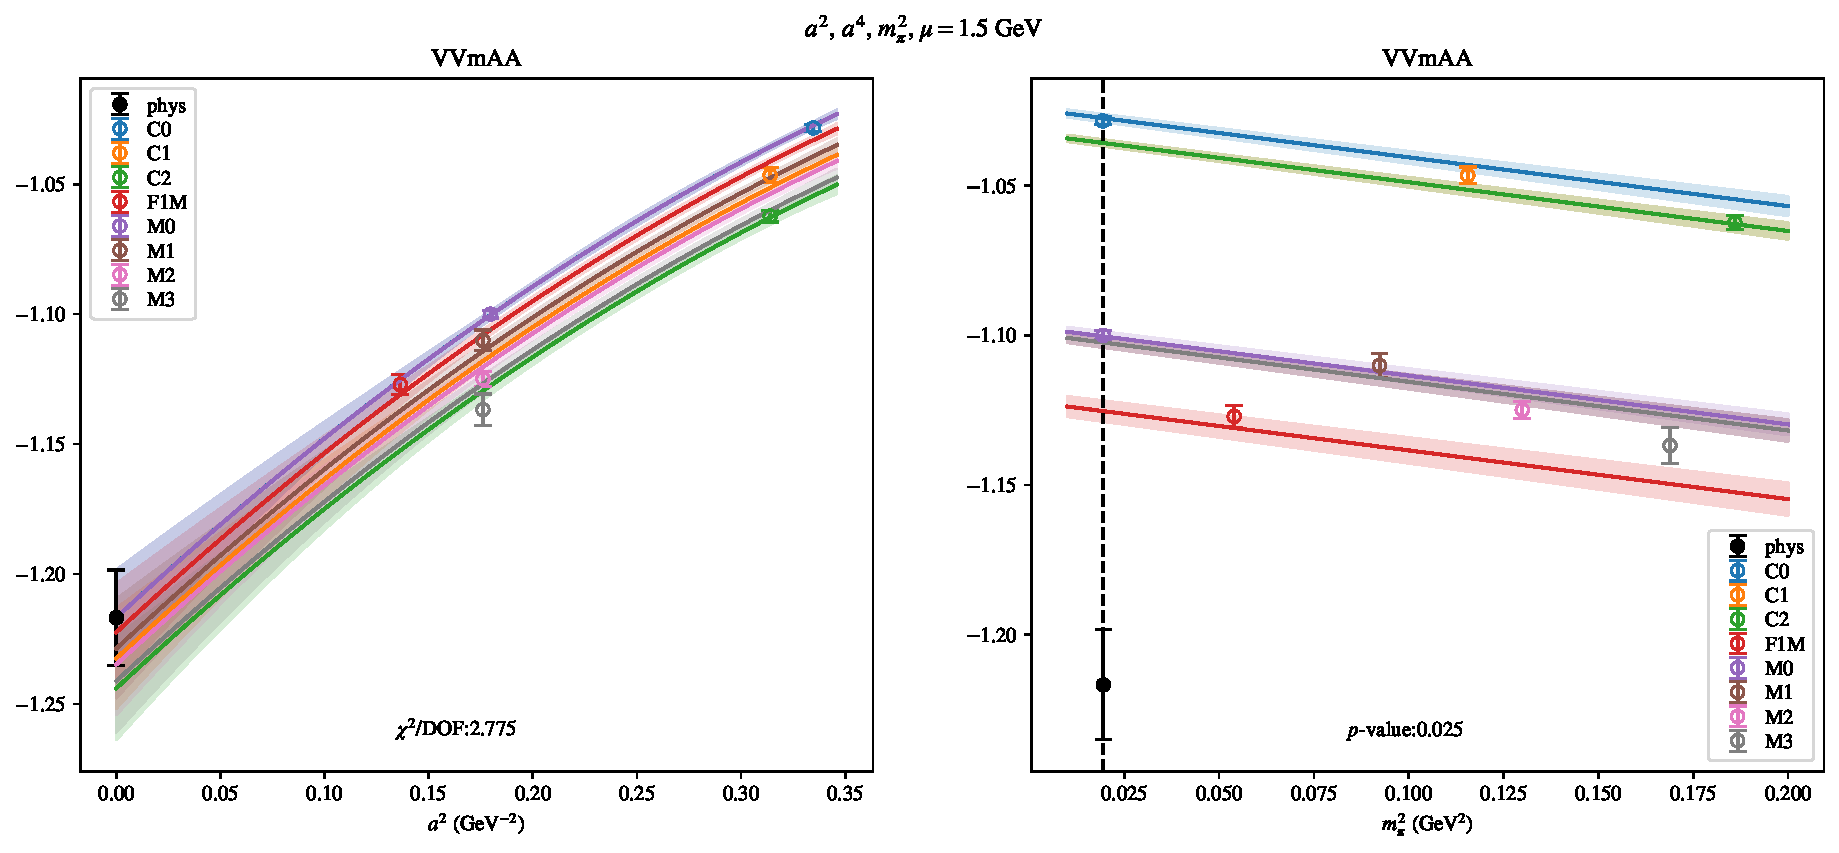
\includepdf[link, pages=-]{VVmAA/NPR/a2a4m2_15.pdf}
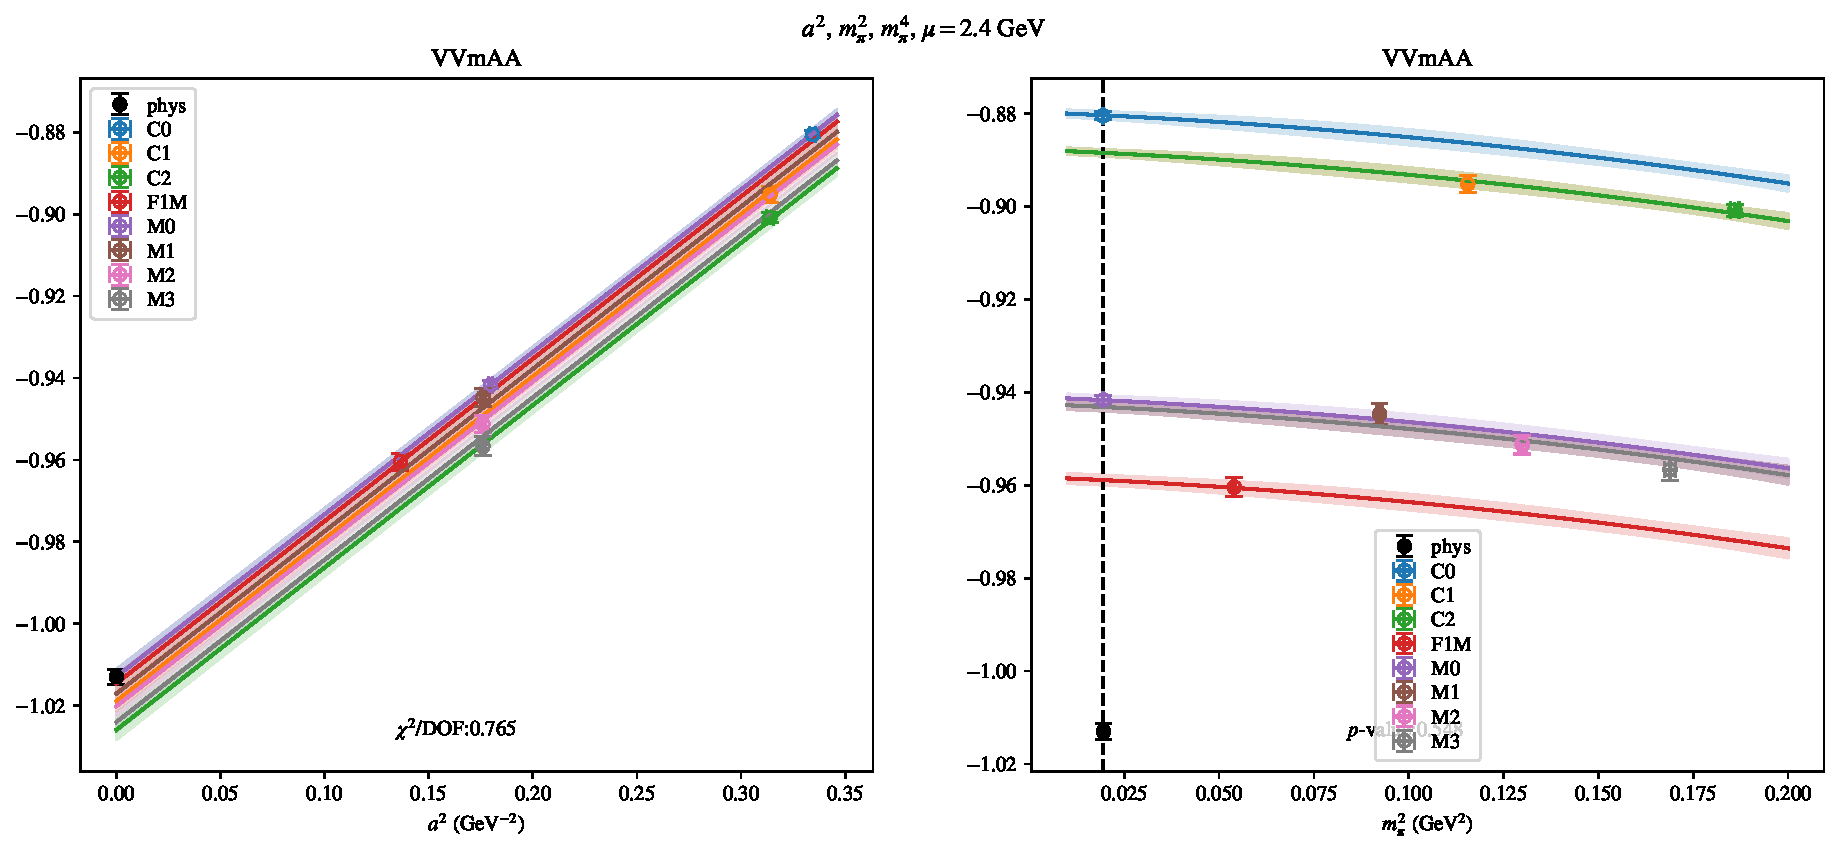
\includepdf[link, pages=-]{VVmAA/NPR/a2m2m4_24.pdf}
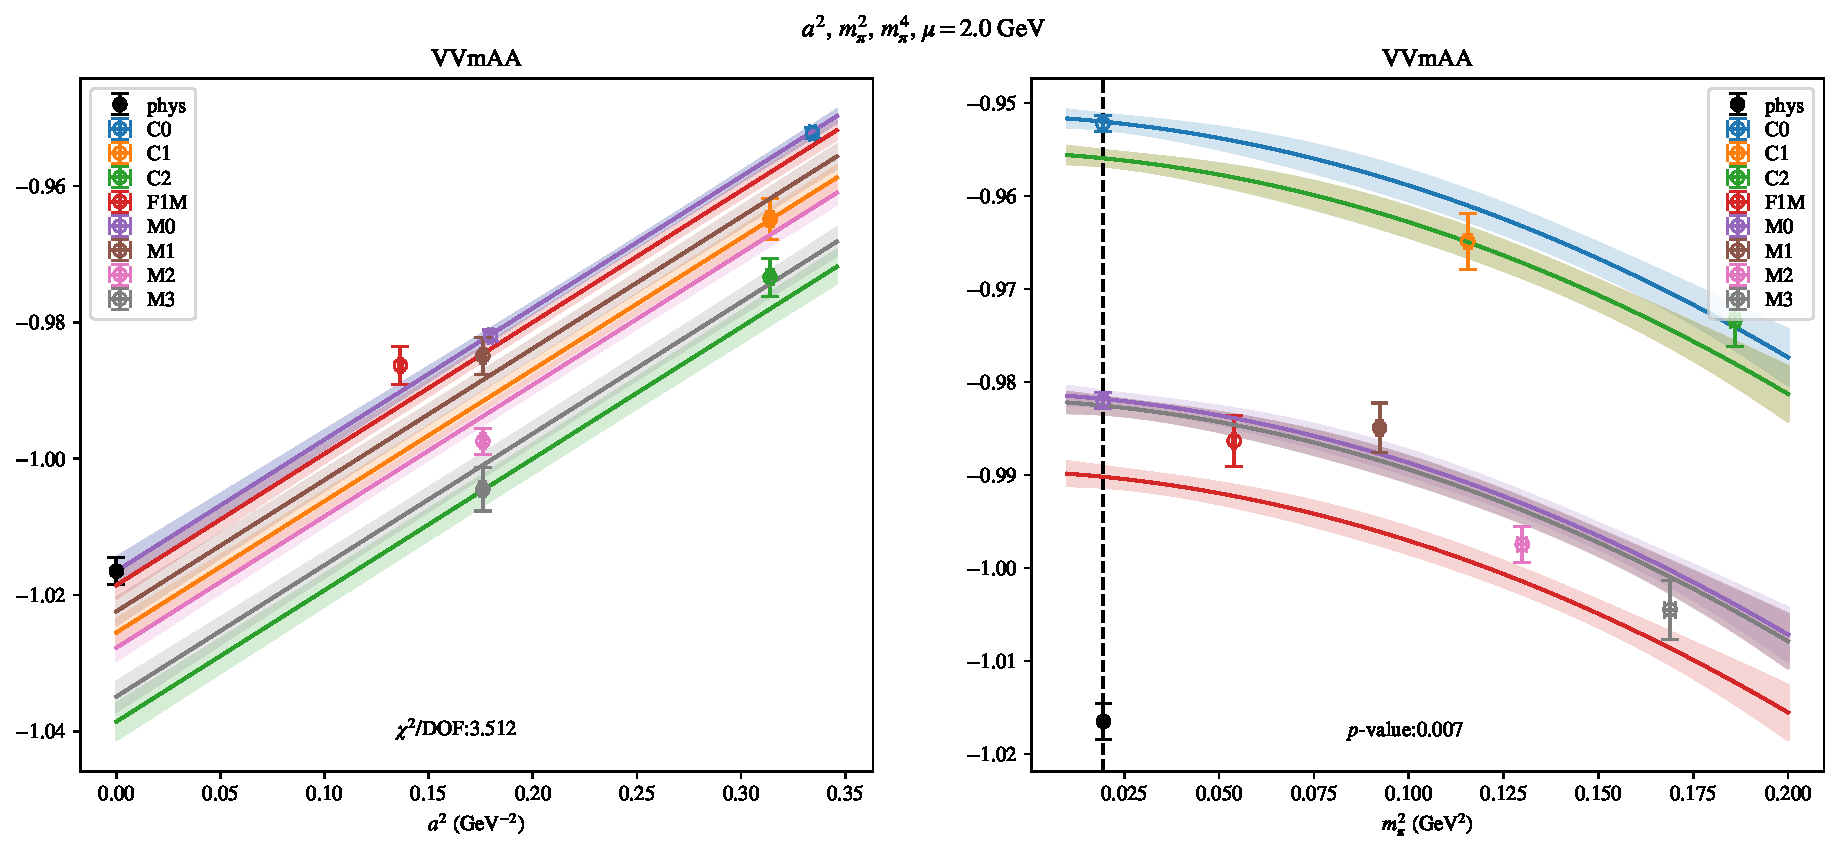
\includepdf[link, pages=-]{VVmAA/NPR/a2m2m4_20.pdf}
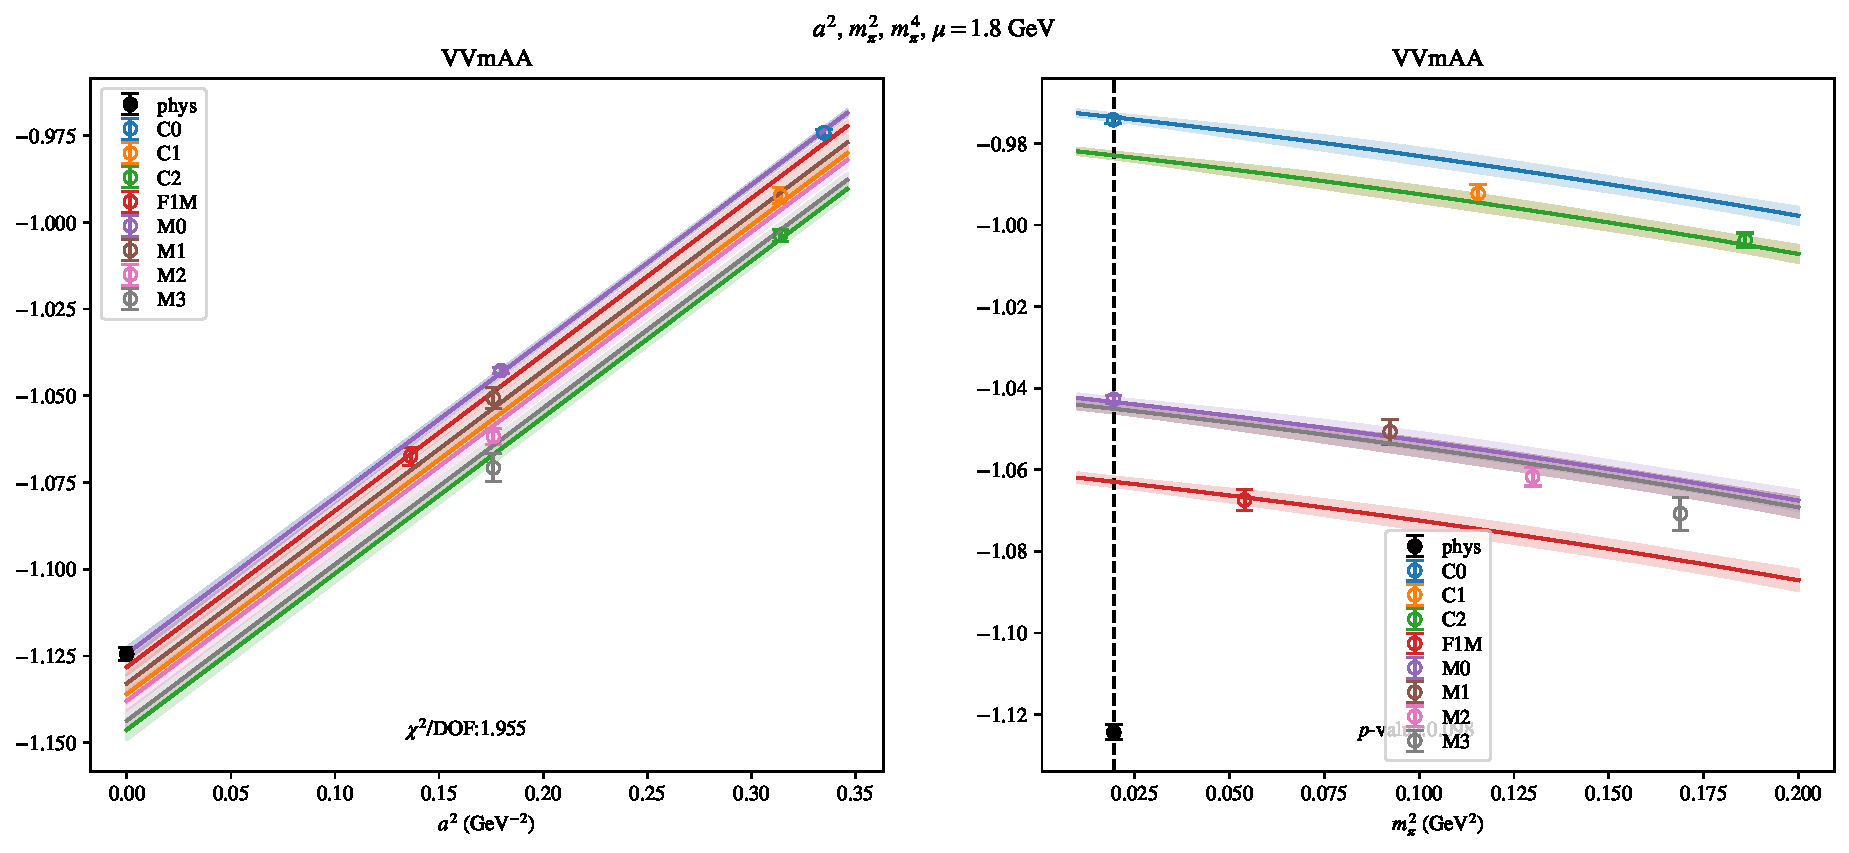
\includepdf[link, pages=-]{VVmAA/NPR/a2m2m4_18.pdf}
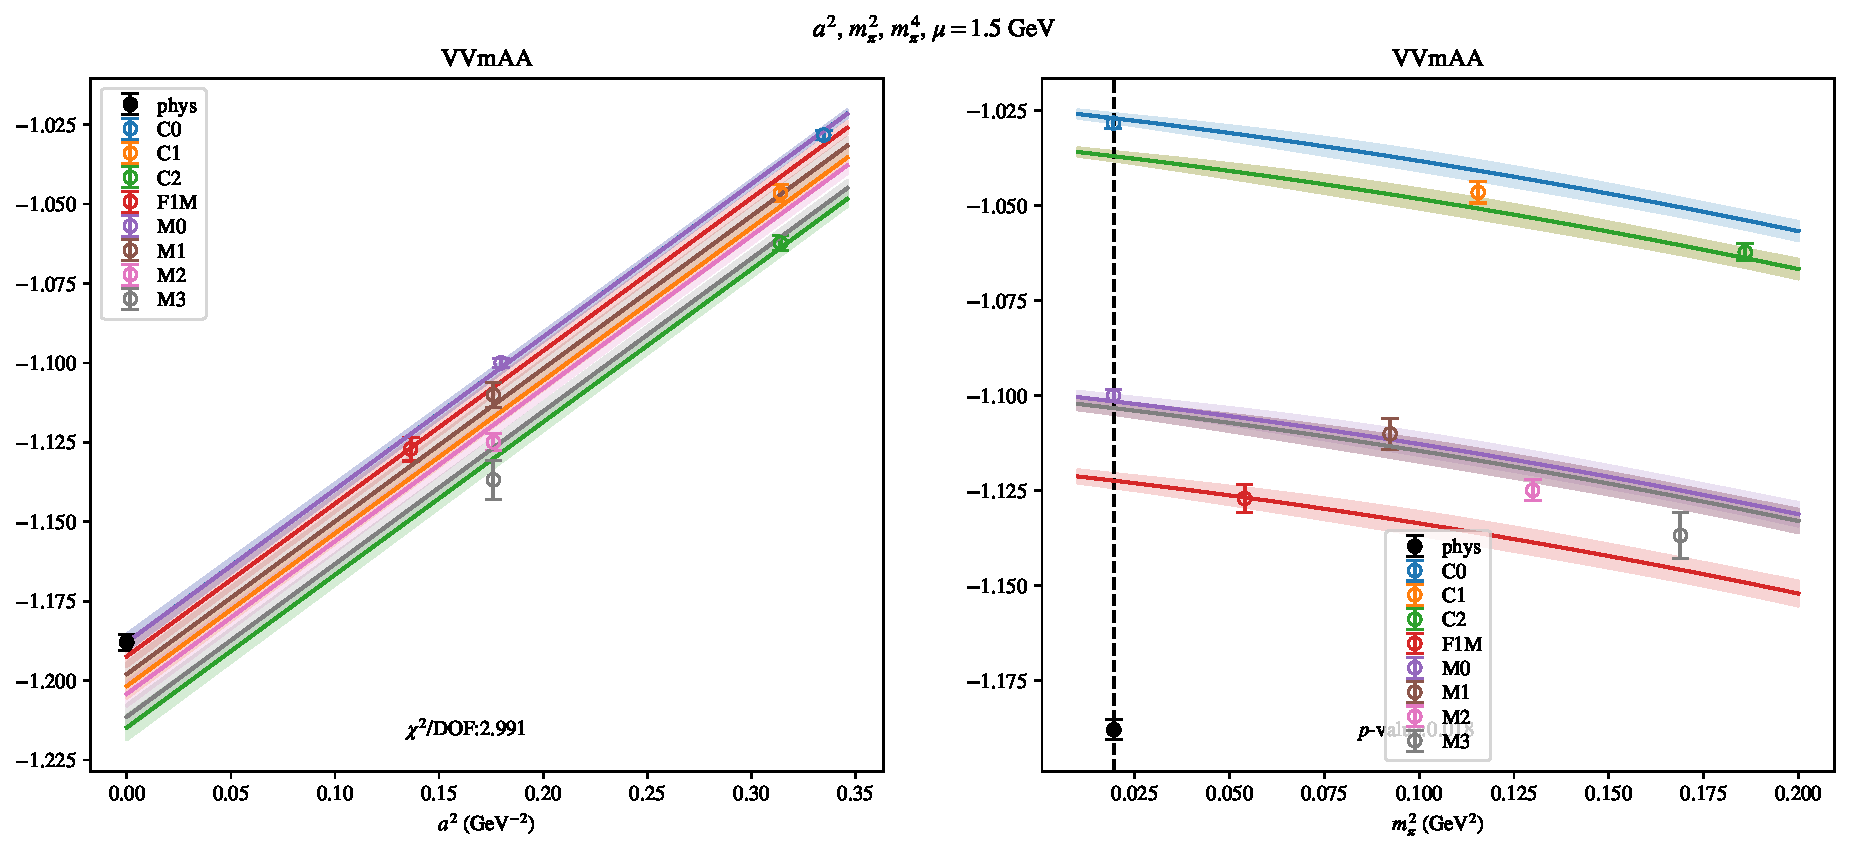
\includepdf[link, pages=-]{VVmAA/NPR/a2m2m4_15.pdf}
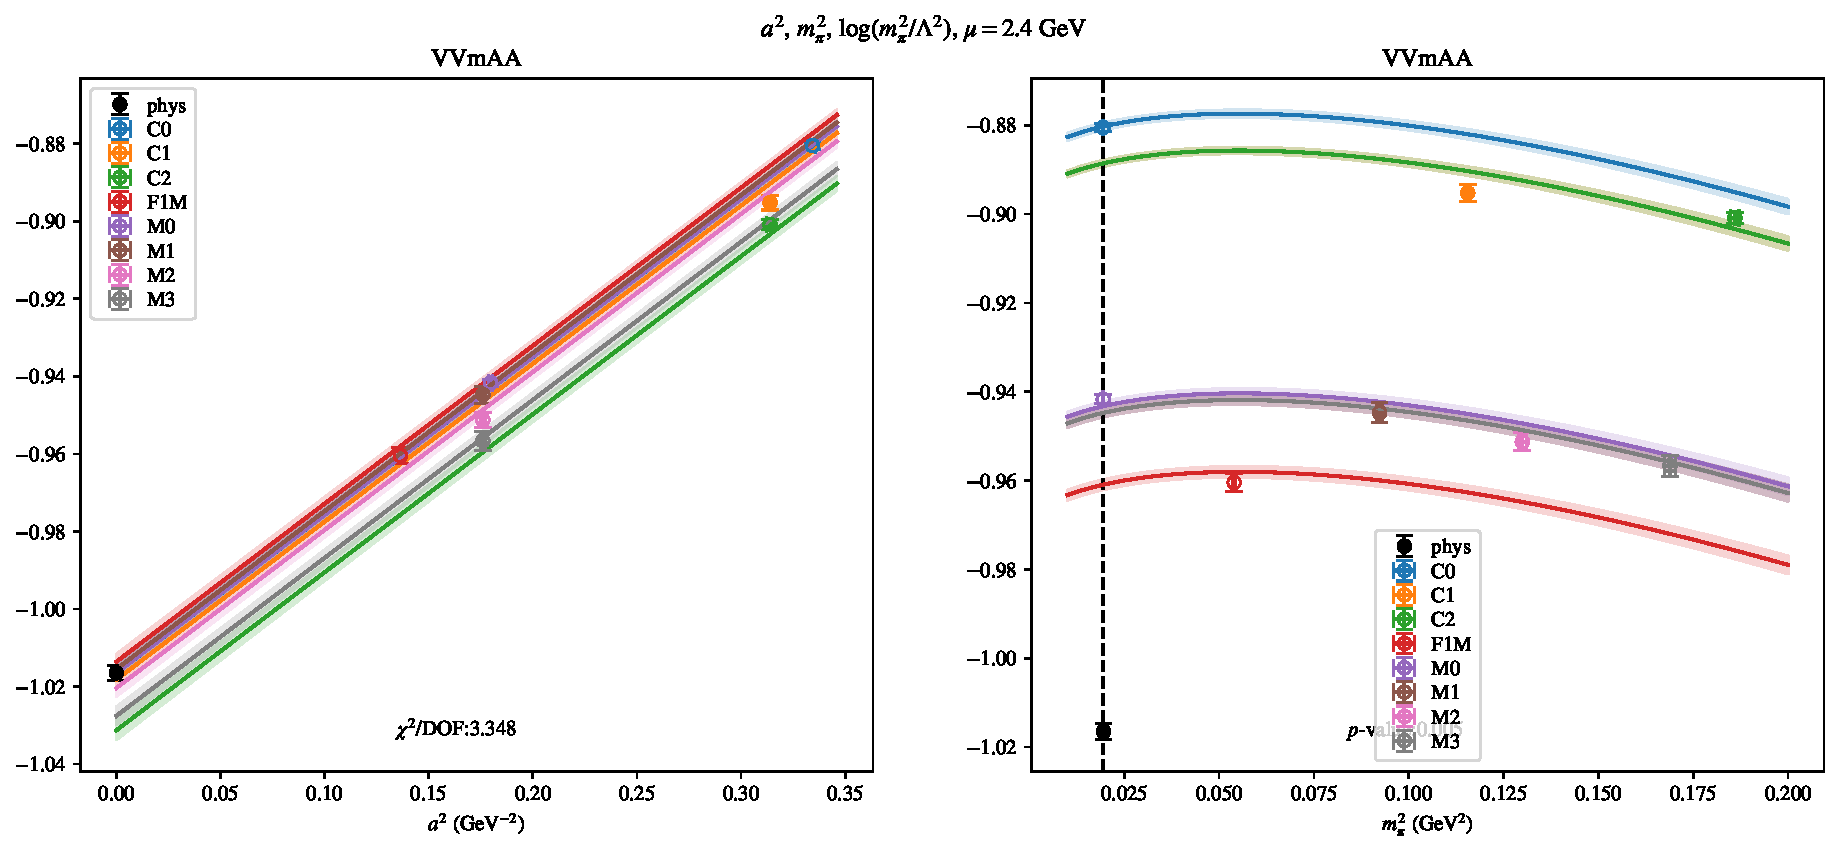
\includepdf[link, pages=-]{VVmAA/NPR/a2m2logm2_24.pdf}
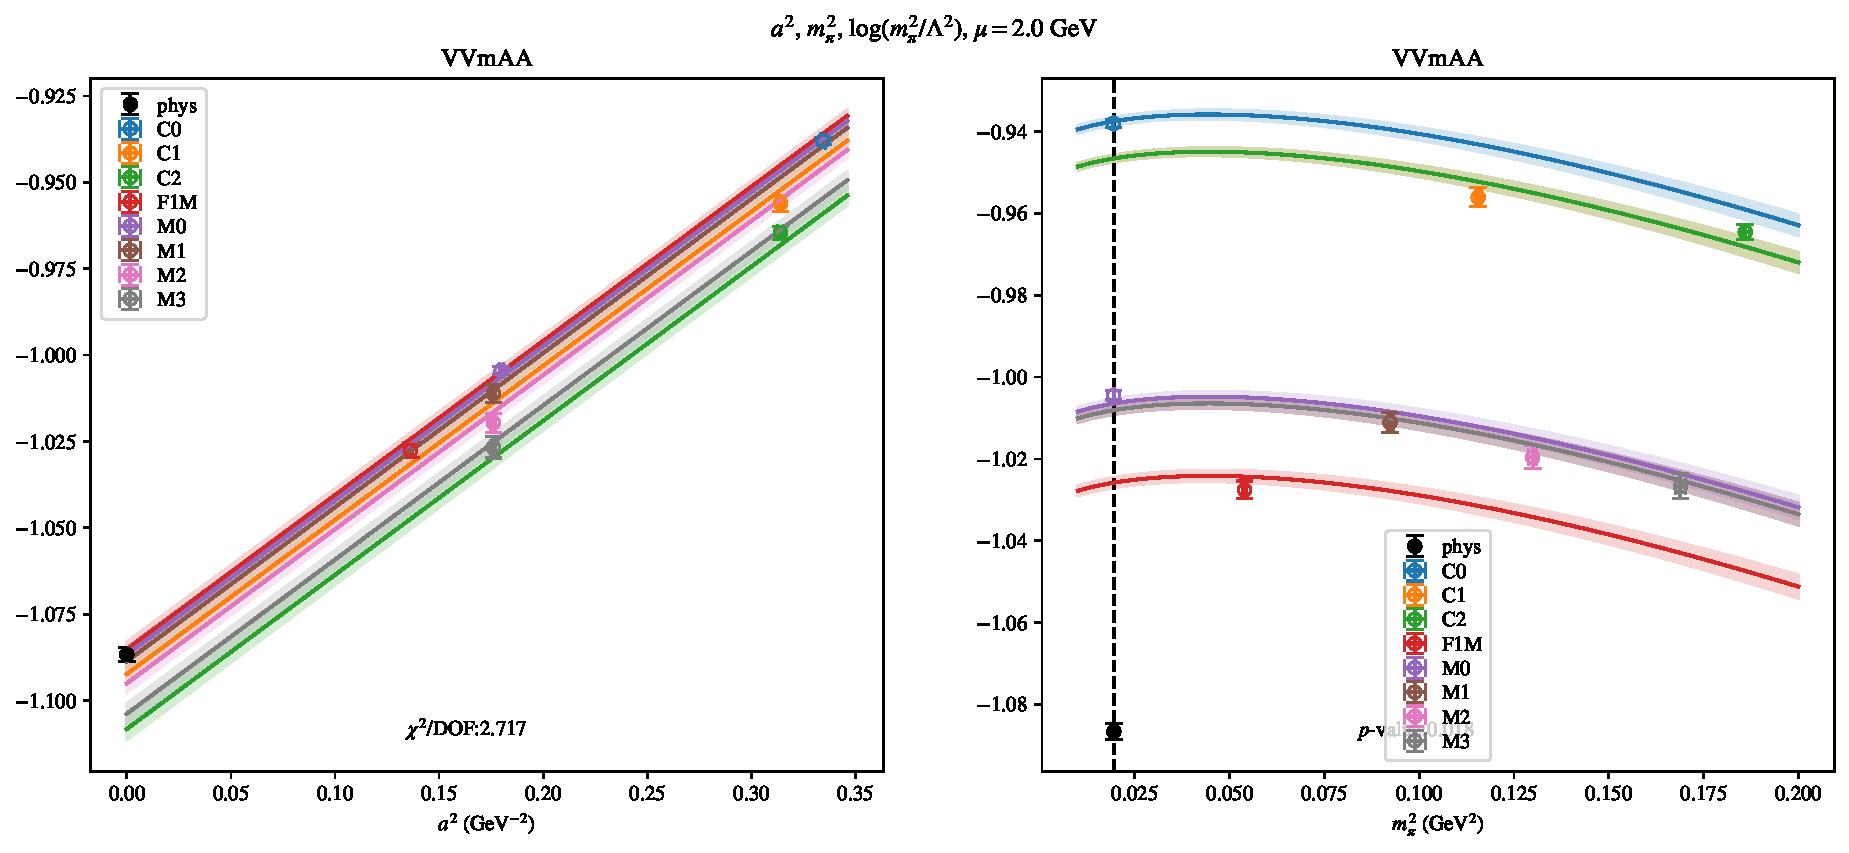
\includepdf[link, pages=-]{VVmAA/NPR/a2m2logm2_20.pdf}
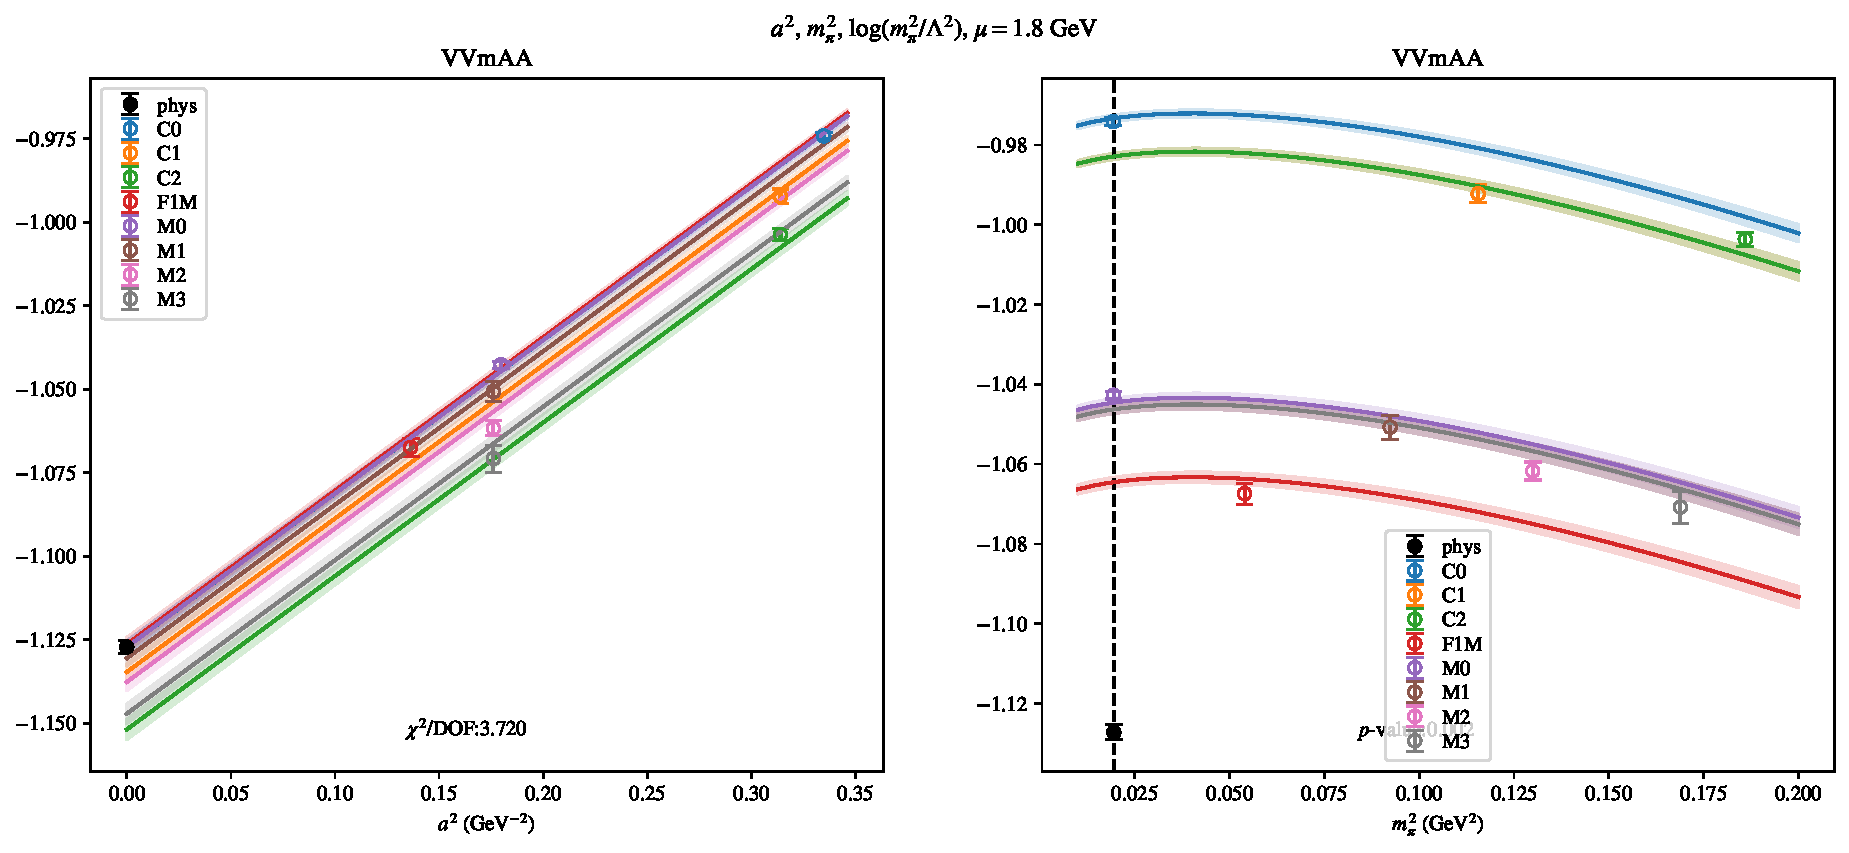
\includepdf[link, pages=-]{VVmAA/NPR/a2m2logm2_18.pdf}
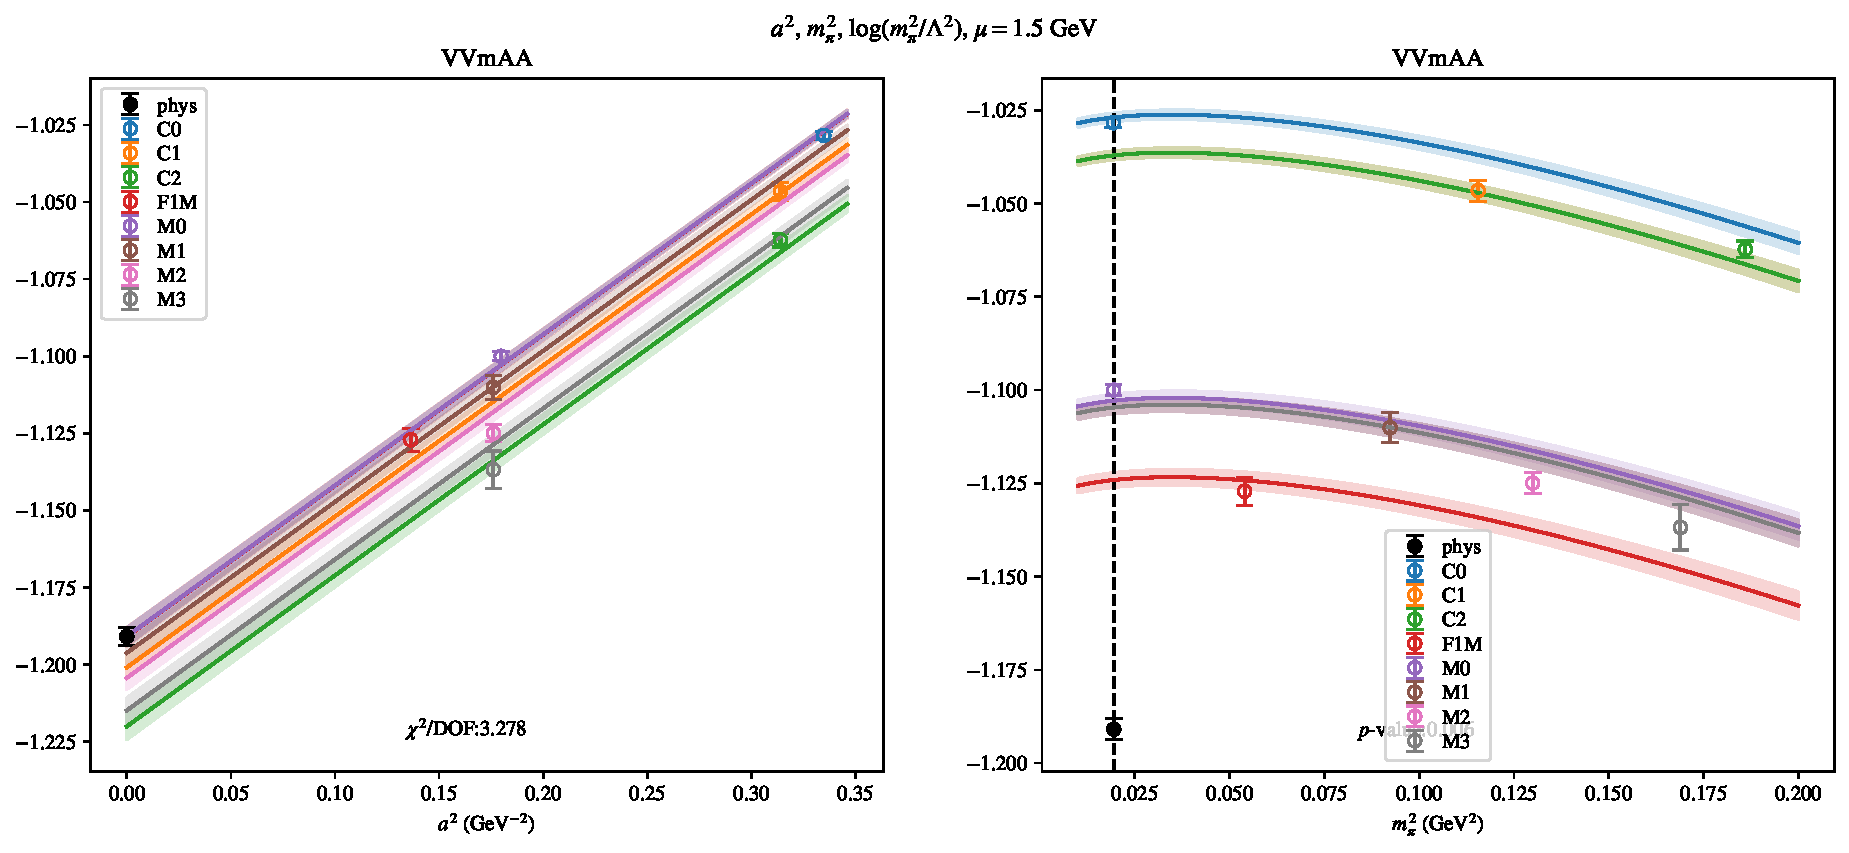
\includepdf[link, pages=-]{VVmAA/NPR/a2m2logm2_15.pdf}
\clearpage
\section{$B_3$}
\begin{table}[h!]
\begin{center}
\begin{tabular}{|c|c|c|c|c|c|}
\hline
$\mu$ (GeV) & $a^2$, $m_\pi^2$& $a^2$, $m_\pi^2$ (no C)& $a^2$, $a^4$, $m_\pi^2$& $a^2$, $m_\pi^2$, $m_\pi^4$& $a^2$, $m_\pi^2$, $\log(m_\pi^2/\Lambda^2)$\\
\hline
2.4& \hyperlink{SSmPP/NPR/a2m2_24.pdf.1}{\textbf{0.9436(13)}: 6.273 (0.0)} & \hyperlink{SSmPP/NPR/a2m2noC_24.pdf.1}{\textbf{0.9086(66)}: 1.786 (0.168)} & \hyperlink{SSmPP/NPR/a2a4m2_24.pdf.1}{\textbf{0.885(10)}: 1.117 (0.346)} & \hyperlink{SSmPP/NPR/a2m2m4_24.pdf.1}{\textbf{0.9453(14)}: 5.797 (0.0)} & \hyperlink{SSmPP/NPR/a2m2logm2_24.pdf.1}{\textbf{0.9266(13)}: 18.643 (0.0)}\\
2.0& \hyperlink{SSmPP/NPR/a2m2_20.pdf.1}{\textbf{0.9557(14)}: 4.069 (0.001)} & \hyperlink{SSmPP/NPR/a2m2noC_20.pdf.1}{\textbf{0.9259(67)}: 1.711 (0.181)} & \hyperlink{SSmPP/NPR/a2a4m2_20.pdf.1}{\textbf{0.906(11)}: 1.012 (0.4)} & \hyperlink{SSmPP/NPR/a2m2m4_20.pdf.1}{\textbf{0.9572(15)}: 3.563 (0.007)} & \hyperlink{SSmPP/NPR/a2m2logm2_20.pdf.1}{\textbf{0.9388(14)}: 13.53 (0.0)}\\
1.8& \hyperlink{SSmPP/NPR/a2m2_18.pdf.1}{\textbf{0.9631(18)}: 2.42 (0.033)} & \hyperlink{SSmPP/NPR/a2m2noC_18.pdf.1}{\textbf{0.9365(74)}: 2.117 (0.12)} & \hyperlink{SSmPP/NPR/a2a4m2_18.pdf.1}{\textbf{0.922(12)}: 1.336 (0.254)} & \hyperlink{SSmPP/NPR/a2m2m4_18.pdf.1}{\textbf{0.9647(17)}: 1.96 (0.098)} & \hyperlink{SSmPP/NPR/a2m2logm2_18.pdf.1}{\textbf{0.9460(18)}: 8.945 (0.0)}\\
1.5& \hyperlink{SSmPP/NPR/a2m2_15.pdf.1}{\textbf{0.9741(27)}: 1.372 (0.231)} & \hyperlink{SSmPP/NPR/a2m2noC_15.pdf.1}{\textbf{0.9523(94)}: 2.007 (0.134)} & \hyperlink{SSmPP/NPR/a2a4m2_15.pdf.1}{\textbf{0.947(15)}: 1.41 (0.228)} & \hyperlink{SSmPP/NPR/a2m2m4_15.pdf.1}{\textbf{0.9759(24)}: 1.054 (0.378)} & \hyperlink{SSmPP/NPR/a2m2logm2_15.pdf.1}{\textbf{0.9565(27)}: 4.87 (0.0)}\\
\hline
\end{tabular}
\caption{Physical point value from chiral and continuum extrapolation at renormalisation scale $\mu$. Entries are \textbf{value(error)}: $\chi^2/\text{DOF}$ ($p$-value).}
\end{center}
\end{table}
\begin{table}[h!]
\begin{center}
\begin{tabular}{|c c|c|c|c|c|c|}
\hline
$\mu$ (GeV) &  & $a^2$, $m_\pi^2$& $a^2$, $m_\pi^2$ (no C)& $a^2$, $a^4$, $m_\pi^2$& $a^2$, $m_\pi^2$, $m_\pi^4$& $a^2$, $m_\pi^2$, $\log(m_\pi^2/\Lambda^2)$\\
\hline
\multirow{2}{0.5in}{2.4} & $\alpha$ & 0.1681(56)& 0.399(44)& 0.76(11)& 0.1609(60)& 0.1834(56)\\
 & $\beta$ & -0.0001(12)& -0.0001(22)& -0.0003(14)& -0.0020(64)& -0.0048(12)\\
\hline
\multirow{2}{0.5in}{2.0} & $\alpha$ & 0.1378(56)& 0.330(43)& 0.63(11)& 0.1316(60)& 0.1515(56)\\
 & $\beta$ & 0.00023(15)& 0.00022(29)& 0.0& -0.0016(71)& -0.0045(16)\\
\hline
\multirow{2}{0.5in}{1.8} & $\alpha$ & 0.1270(59)& 0.295(46)& 0.52(12)& 0.1206(60)& 0.1410(59)\\
 & $\beta$ & 0.00049(17)& 0.00053(30)& 0.00036(19)& -0.0013(74)& -0.0043(17)\\
\hline
\multirow{2}{0.5in}{1.5} & $\alpha$ & 0.1119(69)& 0.245(53)& 0.36(14)& 0.1047(64)& 0.1262(70)\\
 & $\beta$ & 0.00086(20)& 0.00102(36)& 0.00078(23)& -0.0010(90)& -0.0039(20)\\
\hline
\end{tabular}
\caption{Fit values of coefficients in $B = B_0(1 + \mathbf{\alpha} a^2 + \mathbf{\beta} \frac{m_\pi^2}{f_\pi^2} + \ldots)$.}
\end{center}
\end{table}
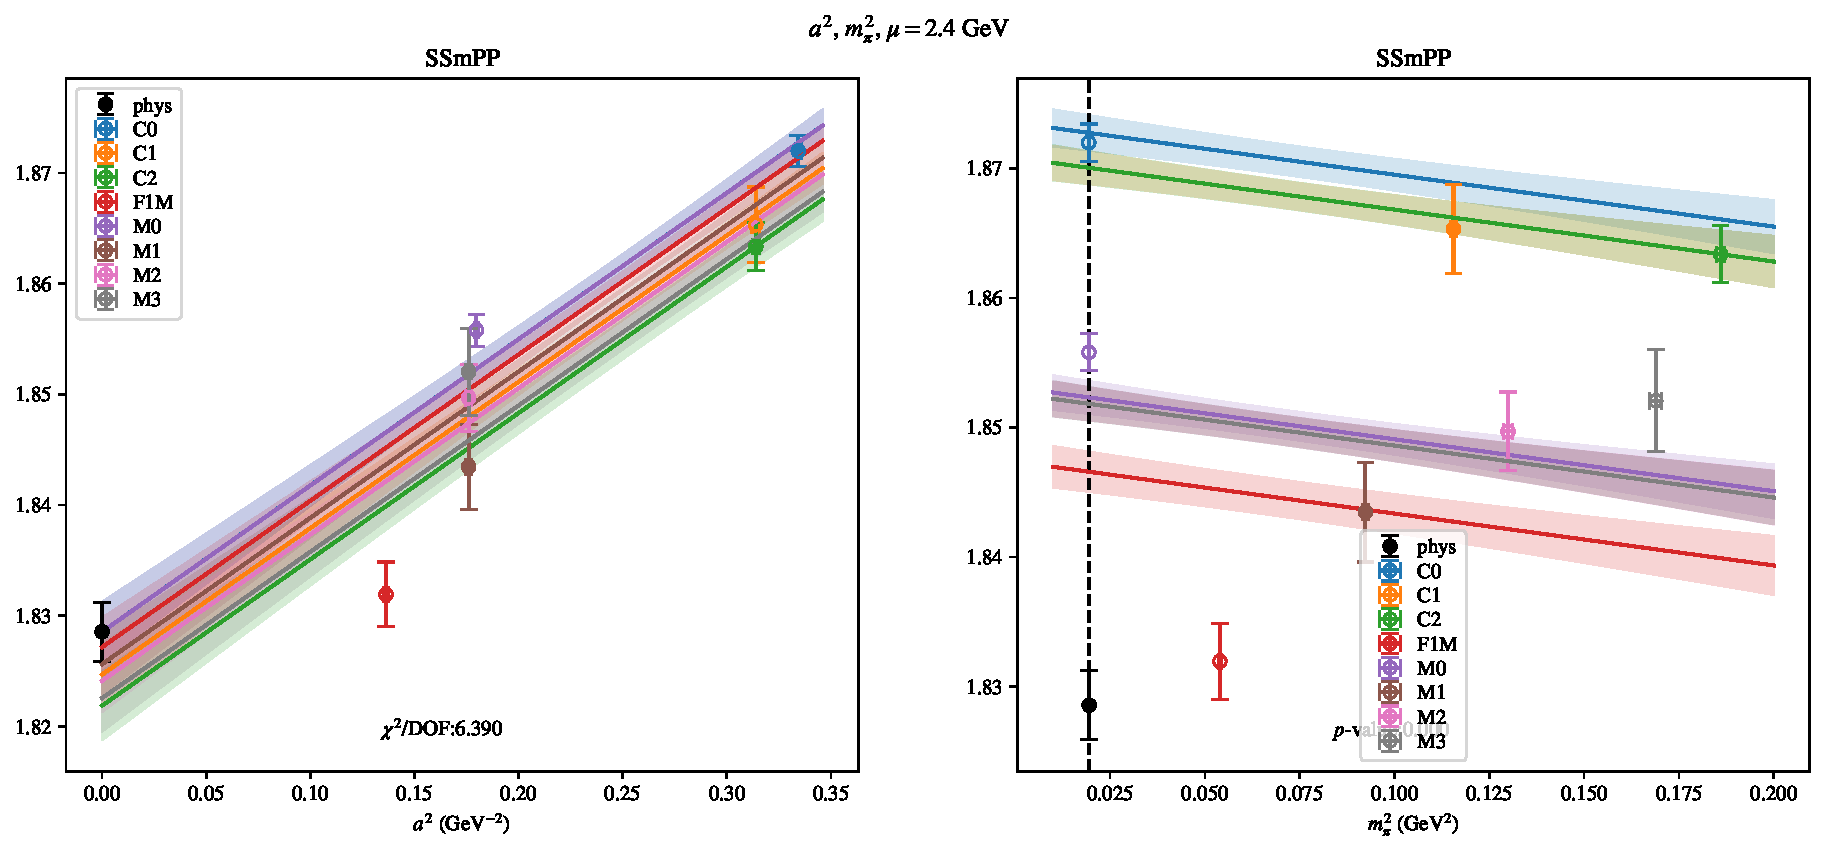
\includepdf[link, pages=-]{SSmPP/NPR/a2m2_24.pdf}
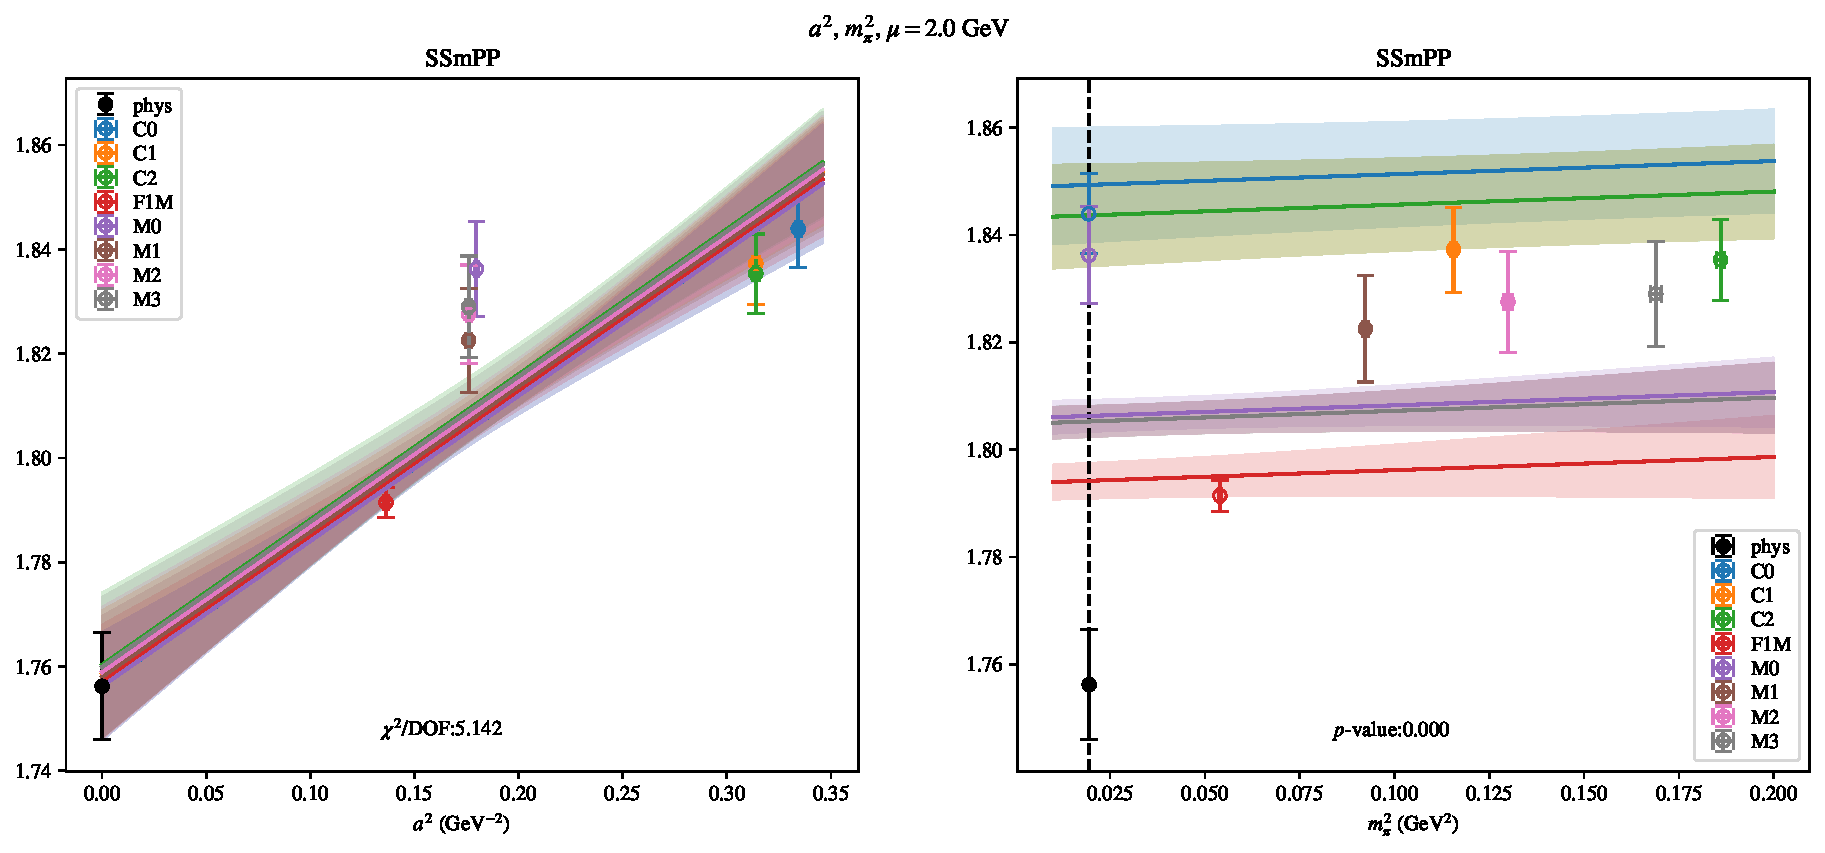
\includepdf[link, pages=-]{SSmPP/NPR/a2m2_20.pdf}
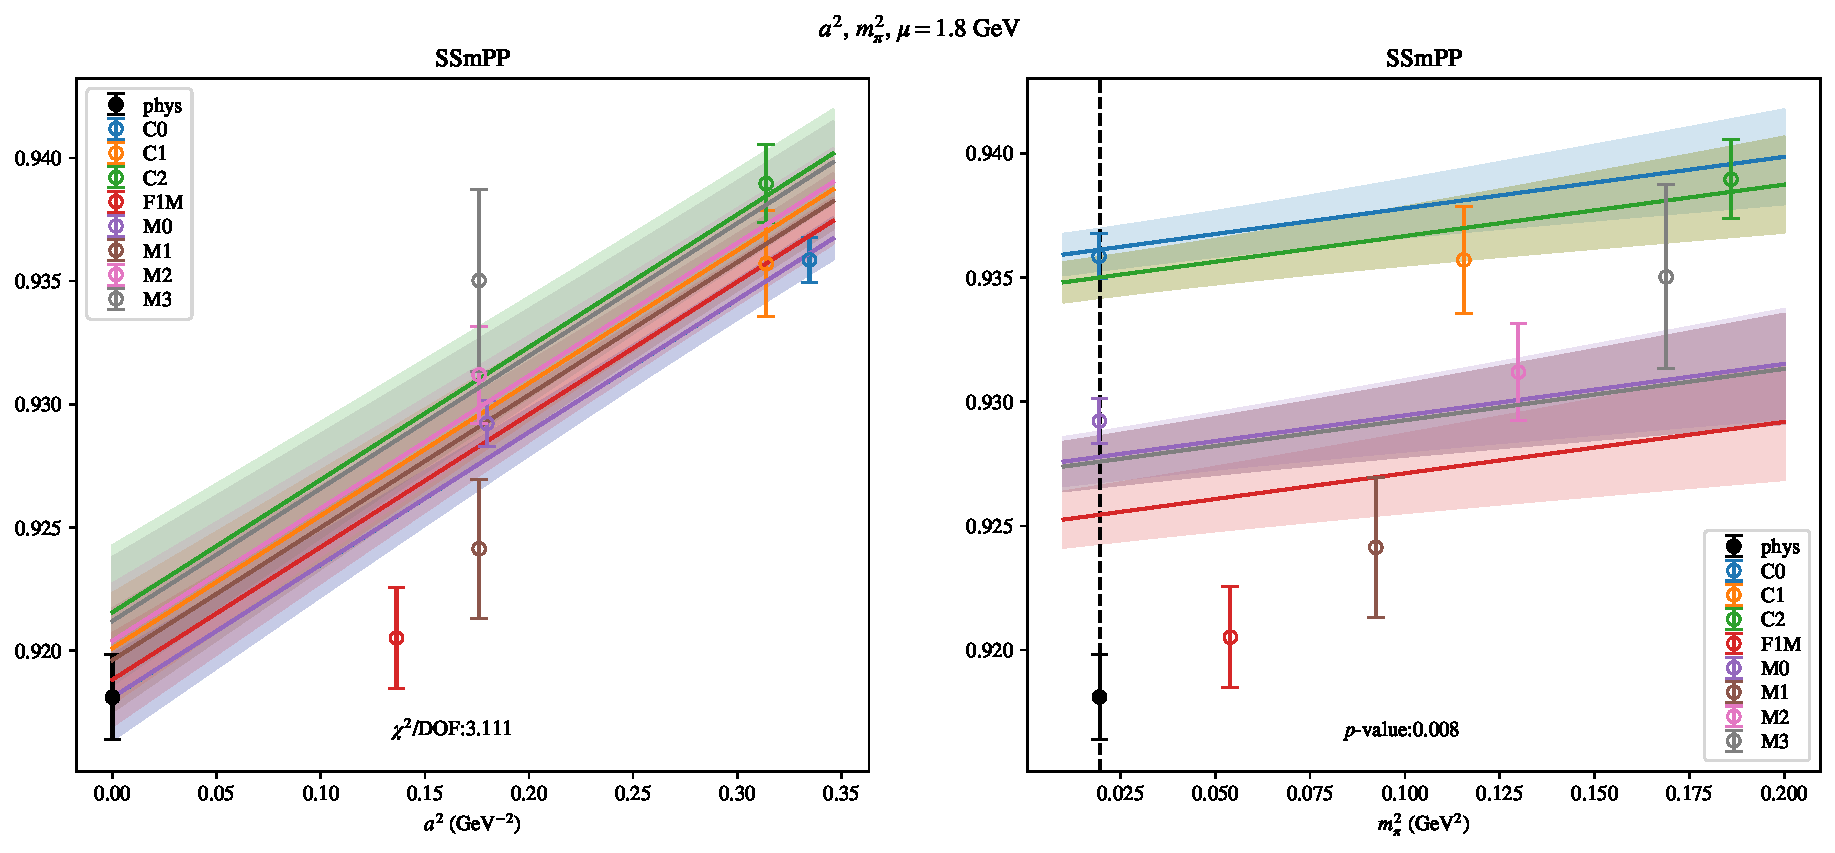
\includepdf[link, pages=-]{SSmPP/NPR/a2m2_18.pdf}
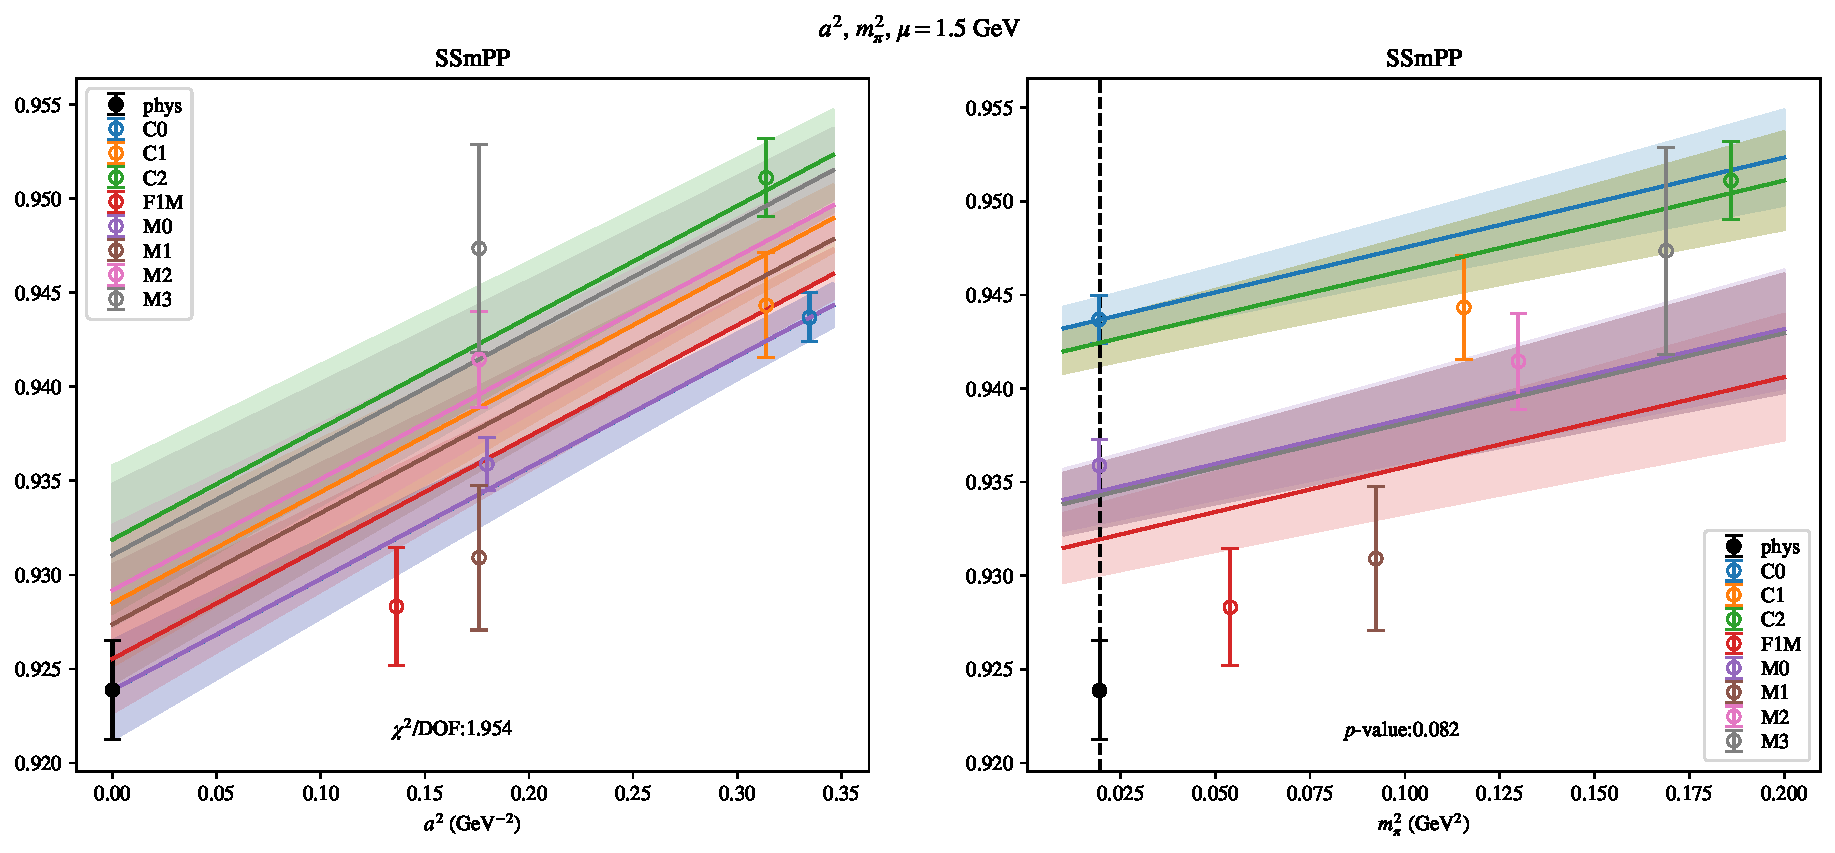
\includepdf[link, pages=-]{SSmPP/NPR/a2m2_15.pdf}
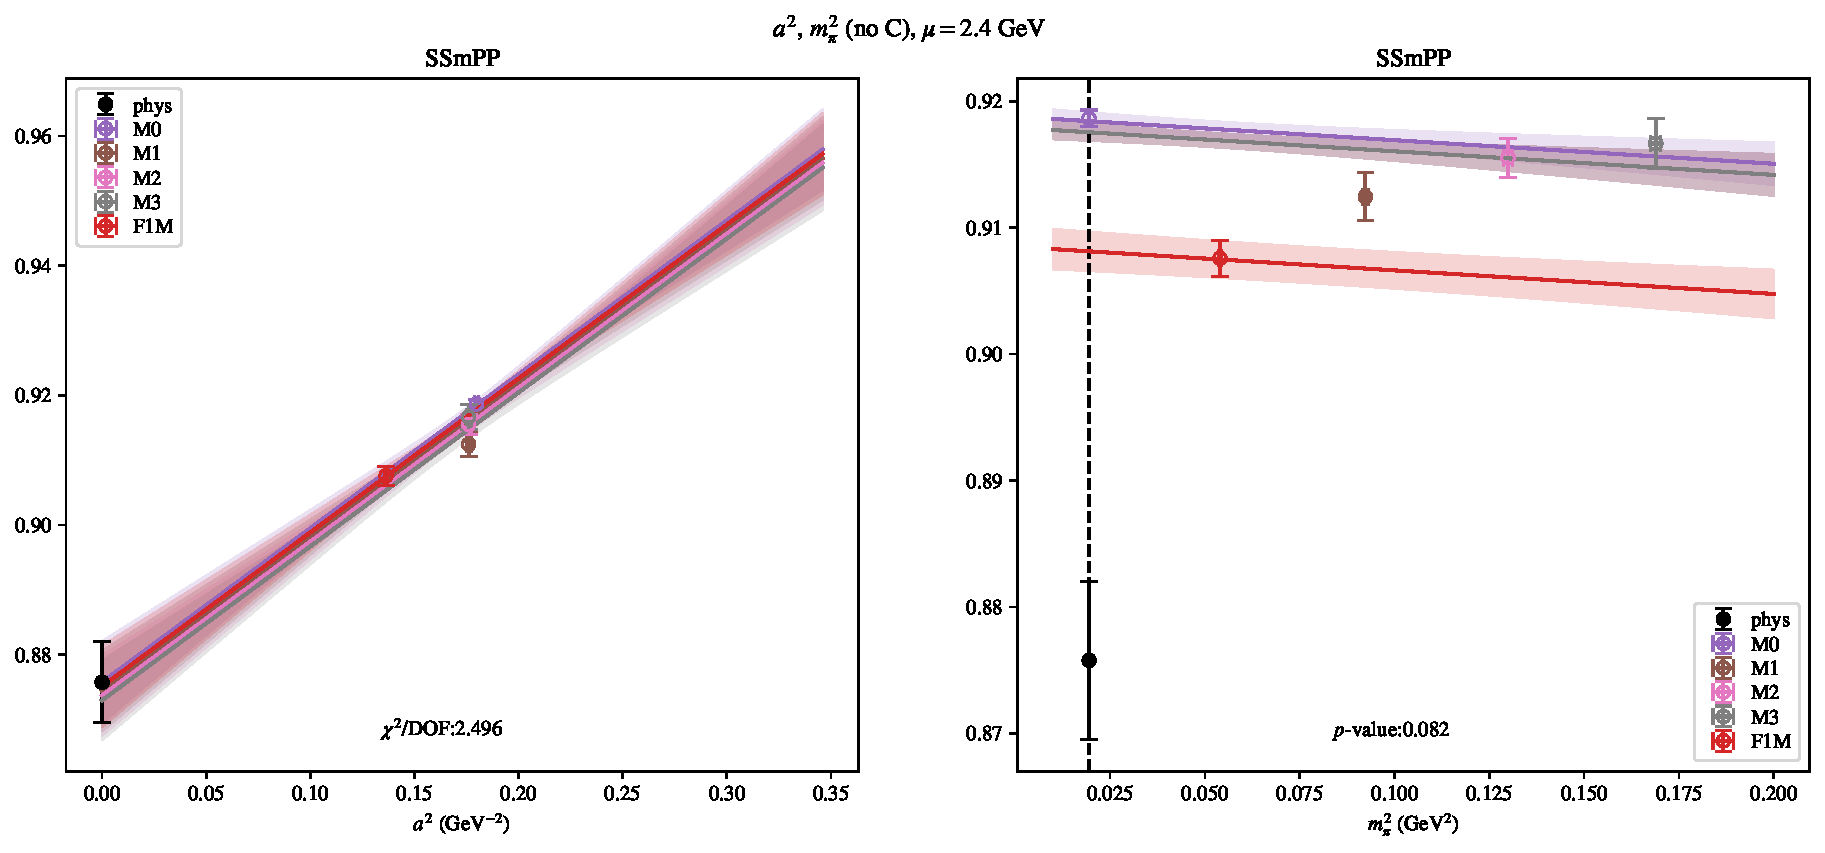
\includepdf[link, pages=-]{SSmPP/NPR/a2m2noC_24.pdf}
\includepdf[link, pages=-]{SSmPP/NPR/a2m2noC_20.pdf}
\includepdf[link, pages=-]{SSmPP/NPR/a2m2noC_18.pdf}
\includepdf[link, pages=-]{SSmPP/NPR/a2m2noC_15.pdf}
\includepdf[link, pages=-]{SSmPP/NPR/a2a4m2_24.pdf}
\includepdf[link, pages=-]{SSmPP/NPR/a2a4m2_20.pdf}
\includepdf[link, pages=-]{SSmPP/NPR/a2a4m2_18.pdf}
\includepdf[link, pages=-]{SSmPP/NPR/a2a4m2_15.pdf}
\includepdf[link, pages=-]{SSmPP/NPR/a2m2m4_24.pdf}
\includepdf[link, pages=-]{SSmPP/NPR/a2m2m4_20.pdf}
\includepdf[link, pages=-]{SSmPP/NPR/a2m2m4_18.pdf}
\includepdf[link, pages=-]{SSmPP/NPR/a2m2m4_15.pdf}
\includepdf[link, pages=-]{SSmPP/NPR/a2m2logm2_24.pdf}
\includepdf[link, pages=-]{SSmPP/NPR/a2m2logm2_20.pdf}
\includepdf[link, pages=-]{SSmPP/NPR/a2m2logm2_18.pdf}
\includepdf[link, pages=-]{SSmPP/NPR/a2m2logm2_15.pdf}
\clearpage
\section{$B_4$}
\begin{table}[h!]
\begin{center}
\begin{tabular}{|c|c|c|c|c|c|}
\hline
$\mu$ (GeV) & $a^2$, $m_\pi^2$& $a^2$, $m_\pi^2$ (no C)& $a^2$, $a^4$, $m_\pi^2$& $a^2$, $m_\pi^2$, $m_\pi^4$& $a^2$, $m_\pi^2$, $\log(m_\pi^2/\Lambda^2)$\\
\hline
2.4& \hyperlink{SSpPP/NPR/a2m2_24.pdf.1}{\textbf{0.53833(89)}: 5.538 (0.0)} & \hyperlink{SSpPP/NPR/a2m2noC_24.pdf.1}{\textbf{0.5585(52)}: 1.377 (0.252)} & \hyperlink{SSpPP/NPR/a2a4m2_24.pdf.1}{\textbf{0.5565(86)}: 5.756 (0.0)} & \hyperlink{SSpPP/NPR/a2m2m4_24.pdf.1}{\textbf{0.53751(95)}: 5.517 (0.0)} & \hyperlink{SSpPP/NPR/a2m2logm2_24.pdf.1}{\textbf{0.54787(91)}: 14.558 (0.0)}\\
2.0& \hyperlink{SSpPP/NPR/a2m2_20.pdf.1}{\textbf{0.56754(98)}: 4.716 (0.0)} & \hyperlink{SSpPP/NPR/a2m2noC_20.pdf.1}{\textbf{0.5922(55)}: 0.797 (0.451)} & \hyperlink{SSpPP/NPR/a2a4m2_20.pdf.1}{\textbf{0.5969(91)}: 3.427 (0.008)} & \hyperlink{SSpPP/NPR/a2m2m4_20.pdf.1}{\textbf{0.5666(10)}: 4.48 (0.001)} & \hyperlink{SSpPP/NPR/a2m2logm2_20.pdf.1}{\textbf{0.57742(99)}: 12.333 (0.0)}\\
1.8& \hyperlink{SSpPP/NPR/a2m2_18.pdf.1}{\textbf{0.5840(12)}: 3.149 (0.008)} & \hyperlink{SSpPP/NPR/a2m2noC_18.pdf.1}{\textbf{0.6114(59)}: 0.41 (0.664)} & \hyperlink{SSpPP/NPR/a2a4m2_18.pdf.1}{\textbf{0.6210(99)}: 1.37 (0.242)} & \hyperlink{SSpPP/NPR/a2m2m4_18.pdf.1}{\textbf{0.5832(11)}: 3.371 (0.009)} & \hyperlink{SSpPP/NPR/a2m2logm2_18.pdf.1}{\textbf{0.5943(12)}: 8.019 (0.0)}\\
1.5& \hyperlink{SSpPP/NPR/a2m2_15.pdf.1}{\textbf{0.6089(17)}: 1.887 (0.093)} & \hyperlink{SSpPP/NPR/a2m2noC_15.pdf.1}{\textbf{0.6400(71)}: 0.233 (0.792)} & \hyperlink{SSpPP/NPR/a2a4m2_15.pdf.1}{\textbf{0.657(12)}: 0.272 (0.896)} & \hyperlink{SSpPP/NPR/a2m2m4_15.pdf.1}{\textbf{0.6084(15)}: 2.247 (0.061)} & \hyperlink{SSpPP/NPR/a2m2logm2_15.pdf.1}{\textbf{0.6199(18)}: 4.156 (0.001)}\\
\hline
\end{tabular}
\caption{Physical point value from chiral and continuum extrapolation at renormalisation scale $\mu$. Entries are \textbf{value(error)}: $\chi^2/\text{DOF}$ ($p$-value).}
\end{center}
\end{table}
\begin{table}[h!]
\begin{center}
\begin{tabular}{|c c|c|c|c|c|c|}
\hline
$\mu$ (GeV) &  & $a^2$, $m_\pi^2$& $a^2$, $m_\pi^2$ (no C)& $a^2$, $a^4$, $m_\pi^2$& $a^2$, $m_\pi^2$, $m_\pi^4$& $a^2$, $m_\pi^2$, $\log(m_\pi^2/\Lambda^2)$\\
\hline
\multirow{2}{0.5in}{2.4} & $\alpha$ & 0.4261(69)& 0.205(56)& 0.11(14)& 0.4334(77)& 0.4100(68)\\
 & $\beta$ & 0.00765(14)& 0.00685(23)& 0.00751(15)& 0.00953(77)& 0.01234(14)\\
\hline
\multirow{2}{0.5in}{2.0} & $\alpha$ & 0.3507(67)& 0.096(54)& -0.1(13)& 0.3581(75)& 0.3364(67)\\
 & $\beta$ & 0.00799(18)& 0.00723(30)& 0.00774(17)& 0.01010(85)& 0.01272(17)\\
\hline
\multirow{2}{0.5in}{1.8} & $\alpha$ & 0.3254(70)& 0.052(56)& -0.2(13)& 0.3312(75)& 0.3104(69)\\
 & $\beta$ & 0.00812(19)& 0.00748(31)& 0.00782(18)& 0.00967(87)& 0.01287(19)\\
\hline
\multirow{2}{0.5in}{1.5} & $\alpha$ & 0.2889(77)& -0.008& -0.3(15)& 0.2926(76)& 0.2734(76)\\
 & $\beta$ & 0.00829(22)& 0.00784(37)& 0.00792(18)& 0.0092(10)& 0.01303(22)\\
\hline
\end{tabular}
\caption{Fit values of coefficients in $B = B_0(1 + \mathbf{\alpha} a^2 + \mathbf{\beta} \frac{m_\pi^2}{f_\pi^2} + \ldots)$.}
\end{center}
\end{table}
\includepdf[link, pages=-]{SSpPP/NPR/a2m2_24.pdf}
\includepdf[link, pages=-]{SSpPP/NPR/a2m2_20.pdf}
\includepdf[link, pages=-]{SSpPP/NPR/a2m2_18.pdf}
\includepdf[link, pages=-]{SSpPP/NPR/a2m2_15.pdf}
\includepdf[link, pages=-]{SSpPP/NPR/a2m2noC_24.pdf}
\includepdf[link, pages=-]{SSpPP/NPR/a2m2noC_20.pdf}
\includepdf[link, pages=-]{SSpPP/NPR/a2m2noC_18.pdf}
\includepdf[link, pages=-]{SSpPP/NPR/a2m2noC_15.pdf}
\includepdf[link, pages=-]{SSpPP/NPR/a2a4m2_24.pdf}
\includepdf[link, pages=-]{SSpPP/NPR/a2a4m2_20.pdf}
\includepdf[link, pages=-]{SSpPP/NPR/a2a4m2_18.pdf}
\includepdf[link, pages=-]{SSpPP/NPR/a2a4m2_15.pdf}
\includepdf[link, pages=-]{SSpPP/NPR/a2m2m4_24.pdf}
\includepdf[link, pages=-]{SSpPP/NPR/a2m2m4_20.pdf}
\includepdf[link, pages=-]{SSpPP/NPR/a2m2m4_18.pdf}
\includepdf[link, pages=-]{SSpPP/NPR/a2m2m4_15.pdf}
\includepdf[link, pages=-]{SSpPP/NPR/a2m2logm2_24.pdf}
\includepdf[link, pages=-]{SSpPP/NPR/a2m2logm2_20.pdf}
\includepdf[link, pages=-]{SSpPP/NPR/a2m2logm2_18.pdf}
\includepdf[link, pages=-]{SSpPP/NPR/a2m2logm2_15.pdf}
\clearpage
\section{$B_5$}
\begin{table}[h!]
\begin{center}
\begin{tabular}{|c|c|c|c|c|c|}
\hline
$\mu$ (GeV) & $a^2$, $m_\pi^2$& $a^2$, $m_\pi^2$ (no C)& $a^2$, $a^4$, $m_\pi^2$& $a^2$, $m_\pi^2$, $m_\pi^4$& $a^2$, $m_\pi^2$, $\log(m_\pi^2/\Lambda^2)$\\
\hline
2.4& \hyperlink{TT/NPR/a2m2_24.pdf.1}{\textbf{0.52399(82)}: 8.212 (0.0)} & \hyperlink{TT/NPR/a2m2noC_24.pdf.1}{\textbf{0.5570(52)}: 0.839 (0.432)} & \hyperlink{TT/NPR/a2a4m2_24.pdf.1}{\textbf{0.5693(86)}: 3.317 (0.01)} & \hyperlink{TT/NPR/a2m2m4_24.pdf.1}{\textbf{0.52309(82)}: 6.953 (0.0)} & \hyperlink{TT/NPR/a2m2logm2_24.pdf.1}{\textbf{0.53288(83)}: 20.113 (0.0)}\\
2.0& \hyperlink{TT/NPR/a2m2_20.pdf.1}{\textbf{0.5940(10)}: 7.141 (0.0)} & \hyperlink{TT/NPR/a2m2noC_20.pdf.1}{\textbf{0.6355(60)}: 0.563 (0.569)} & \hyperlink{TT/NPR/a2a4m2_20.pdf.1}{\textbf{0.658(10)}: 1.281 (0.275)} & \hyperlink{TT/NPR/a2m2m4_20.pdf.1}{\textbf{0.5930(10)}: 6.036 (0.0)} & \hyperlink{TT/NPR/a2m2logm2_20.pdf.1}{\textbf{0.6039(10)}: 14.63 (0.0)}\\
1.8& \hyperlink{TT/NPR/a2m2_18.pdf.1}{\textbf{0.6358(17)}: 3.741 (0.002)} & \hyperlink{TT/NPR/a2m2noC_18.pdf.1}{\textbf{0.6796(79)}: 0.363 (0.695)} & \hyperlink{TT/NPR/a2a4m2_18.pdf.1}{\textbf{0.711(13)}: 0.386 (0.819)} & \hyperlink{TT/NPR/a2m2m4_18.pdf.1}{\textbf{0.6345(15)}: 3.542 (0.007)} & \hyperlink{TT/NPR/a2m2logm2_18.pdf.1}{\textbf{0.6468(17)}: 7.548 (0.0)}\\
1.5& \hyperlink{TT/NPR/a2m2_15.pdf.1}{\textbf{0.6990(32)}: 2.017 (0.073)} & \hyperlink{TT/NPR/a2m2noC_15.pdf.1}{\textbf{0.745(12)}: 0.194 (0.823)} & \hyperlink{TT/NPR/a2a4m2_15.pdf.1}{\textbf{0.791(20)}: 0.255 (0.907)} & \hyperlink{TT/NPR/a2m2m4_15.pdf.1}{\textbf{0.6975(26)}: 2.13 (0.074)} & \hyperlink{TT/NPR/a2m2logm2_15.pdf.1}{\textbf{0.7116(32)}: 3.696 (0.002)}\\
\hline
\end{tabular}
\caption{Physical point value from chiral and continuum extrapolation at renormalisation scale $\mu$. Entries are \textbf{value(error)}: $\chi^2/\text{DOF}$ ($p$-value).}
\end{center}
\end{table}
\begin{table}[h!]
\begin{center}
\begin{tabular}{|c c|c|c|c|c|c|}
\hline
$\mu$ (GeV) &  & $a^2$, $m_\pi^2$& $a^2$, $m_\pi^2$ (no C)& $a^2$, $a^4$, $m_\pi^2$& $a^2$, $m_\pi^2$, $m_\pi^4$& $a^2$, $m_\pi^2$, $\log(m_\pi^2/\Lambda^2)$\\
\hline
\multirow{2}{0.5in}{2.4} & $\alpha$ & -0.244(51)& -0.57(48)& -0.9(12)& -0.239(53)& -0.249(50)\\
 & $\beta$ & 0.00685(14)& 0.00633(25)& 0.00656(12)& 0.00962(72)& 0.01156(13)\\
\hline
\multirow{2}{0.5in}{2.0} & $\alpha$ & -0.284(51)& -0.64(48)& -1.1(12)& -0.278(53)& -0.288(51)\\
 & $\beta$ & 0.00728(23)& 0.00685(43)& 0.00685(19)& 0.01082(99)& 0.01205(22)\\
\hline
\multirow{2}{0.5in}{1.8} & $\alpha$ & -0.290(59)& -0.64(55)& -1.2(13)& -0.284(56)& -0.296(59)\\
 & $\beta$ & 0.00713(24)& 0.00708(40)& 0.00674(19)& 0.0100(10)& 0.01189(24)\\
\hline
\multirow{2}{0.5in}{1.5} & $\alpha$ & -0.302(78)& -0.65(72)& -1.3(17)& -0.296(63)& -0.310(76)\\
 & $\beta$ & 0.00700(26)& 0.00741(46)& 0.00661(19)& 0.0094(13)& 0.01173(26)\\
\hline
\end{tabular}
\caption{Fit values of coefficients in $B = B_0(1 + \mathbf{\alpha} a^2 + \mathbf{\beta} \frac{m_\pi^2}{f_\pi^2} + \ldots)$.}
\end{center}
\end{table}
\includepdf[link, pages=-]{TT/NPR/a2m2_24.pdf}
\includepdf[link, pages=-]{TT/NPR/a2m2_20.pdf}
\includepdf[link, pages=-]{TT/NPR/a2m2_18.pdf}
\includepdf[link, pages=-]{TT/NPR/a2m2_15.pdf}
\includepdf[link, pages=-]{TT/NPR/a2m2noC_24.pdf}
\includepdf[link, pages=-]{TT/NPR/a2m2noC_20.pdf}
\includepdf[link, pages=-]{TT/NPR/a2m2noC_18.pdf}
\includepdf[link, pages=-]{TT/NPR/a2m2noC_15.pdf}
\includepdf[link, pages=-]{TT/NPR/a2a4m2_24.pdf}
\includepdf[link, pages=-]{TT/NPR/a2a4m2_20.pdf}
\includepdf[link, pages=-]{TT/NPR/a2a4m2_18.pdf}
\includepdf[link, pages=-]{TT/NPR/a2a4m2_15.pdf}
\includepdf[link, pages=-]{TT/NPR/a2m2m4_24.pdf}
\includepdf[link, pages=-]{TT/NPR/a2m2m4_20.pdf}
\includepdf[link, pages=-]{TT/NPR/a2m2m4_18.pdf}
\includepdf[link, pages=-]{TT/NPR/a2m2m4_15.pdf}
\includepdf[link, pages=-]{TT/NPR/a2m2logm2_24.pdf}
\includepdf[link, pages=-]{TT/NPR/a2m2logm2_20.pdf}
\includepdf[link, pages=-]{TT/NPR/a2m2logm2_18.pdf}
\includepdf[link, pages=-]{TT/NPR/a2m2logm2_15.pdf}
\clearpage
\end{document}